% The main file for developing the proposal. 
% Variants with different class options are 
% - submit.tex (no draft stuff, no ednotes, no revision information)
% - public.tex (like submit.tex, but no financials either) 
\providecommand{\classoptions}{,keys} % to be overwritten in variants
\documentclass[noworkareas,deliverables,gitinfo,report,propB\classoptions]{euproposal}
\usepackage[T1]{fontenc}
\usepackage[utf8]{inputenc}
\addbibresource{../lib/dummy.bib}
%%% institutions
\WAinstitution[id=PS,
        countryshort=FR,
        acronym=UPSud]
        {Universit\'e Paris-Sud}

\WAinstitution[id=LL,
        countryshort=FR,
        acronym=Logilab]
        {Logilab}

\WAinstitution[id=UV,
        countryshort=FR,
        acronym=UVSQ]
        {Universit\'e de Versailles Saint-Quentin}

\WAinstitution[id=UJF,
        countryshort=FR,
        acronym=UGA]
        {Universit\'e Grenoble Alpes}

\WAinstitution[id=UB,
        countryshort=FR,
        acronym=CNRS]
        {CNRS}

\WAinstitution[id=UO,
        countryshort=UK,
        acronym=UOXF]
        {University of Oxford}

\WAinstitution[id=USH,
        countryshort=UK,
        acronym=USFD]
        {University of Sheffield}

\WAinstitution[id=USO,
        countryshort=UK,
        acronym=SOUTHAMPTON]
        {University of Southampton}

\WAinstitution[id=SA,
        countryshort=UK,
        acronym=USTAN]
        {University of St Andrews}

\WAinstitution[id=UW,
        countryshort=UK,
        acronym=UWarwick]
        {University of Warwick}

\WAinstitution[id=JU,
        countryshort=DE,
        acronym=JacobsUni]
        {Jacobs University Bremen}

\WAinstitution[id=FAU,
        countryshort=DE,
        acronym=FAU]
        {Friedrich-Alexander Universit\"at Erlangen/N\"urnberg}

\WAinstitution[id=UK,
        countryshort=DE,
        acronym=UNIKL]
        {University of Kaiserslautern}

\WAinstitution[id=US,
        countryshort=PL,
        acronym=USlaski]
        {University of Silesia}

\WAinstitution[id=ZH,
        countryshort=CH,
        acronym=UZH]
        {Universit\"{a}t Z\"{u}rich}

\WAinstitution[id=SR,
        countryshort=NO,
        acronym=Simula]
        {Simula Research Laboratory}

\WAinstitution[id=UG,
	countryshort=BE,
	acronym=UGent]
	{Ghent University}

\WAinstitution[id=XFEL,
        countryshort=DE,
        acronym=XFEL]
        {European XFEL GmbH}

% \WAinstitution[id=UWS,
%         countryshort=US,
%         acronym=UWS]
%         {University of Washington at Seattle}

% \WAperson[id=miko, 
%            personaltitle=Prof. Dr.,
%            birthdate=13. September 1964,
%            academictitle=Professor of Computer Science,
%            affiliation=jacu,
%            department=case,
%            privaddress=None of your business,
%            privtel=that neither,
%            email=m.kohlhase@jacobs-university.de,
%            workaddress={Campus Ring 1, 28757 Bremen},
%            worktel=+49 421 200 3140,
%            worktelfax=+49 421 200 3140/493140,
%            workfax=+49 421 200 493140]
%            {Michael Kohlhase}

\WAperson[id=thiery,
           personaltitle=Prof. ,
           birthdate=28 Mai 1973,
           academictitle=Professor of Computer Science,
           affiliation=PS,
           department=Laboratoire de Recherche en Informatique,
           privaddress=None of your business,
           privtel=that neither,
           email=Nicolas.Thiery@u-psud.fr,
           workaddress={Campus Ring 1, 28757 Bremen},
           %worktel=+33 6 77 90 32 79,
           worktelfax=+33 6 77 90 32 79,
           %workfax=N/A
           ]
           {Nicolas M. Thiéry}

%%% Local Variables: 
%%% mode: latex
%%% TeX-master: "proposal"
%%% End: 

% LocalWords:  WAperson miko personaltitle academictitle privaddress privtel Sud
% LocalWords:  workaddress worktel workfax gc worktelfax pcg pcsa WAinstitution
% LocalWords:  shortname partof streetaddress townzip countryshort efo 3kd89
% LocalWords:  jacobs-logo.png Seefahrtstrasse Kruislann Montparnasse Universit
% LocalWords:  baz Westerfield
% Some sections of the included files depend on this.

\begin{document}
\begin{center}\color{red}\huge
  This mock proposal is just an example for \texttt{euproposal.cls} it reflects the ICT
  template of January 2012
\end{center}
\begin{proposal}[site=jacu,jacuRM=36,
  site=efo,efoRM=36,
  site=bar,barRM=36,
  site=baz,bazRM=36,
  coordinator=miko,
  acronym={iPoWr},
  acrolong={\underline{I}ntelligent} {\underline{P}r\underline{o}sal} {\underline{Wr}iting},
  title=\pn: \protect\pnlong,
  callname = ICT Call 1,
  callid = FP7-???-200?-?,
  instrument= Small or Medium-Scale Focused Research Project (STREP), 
  challengeid = 4,
  challenge = ICT for EU Proposals,
  objectiveid={ICT-2012.4.4}, 
  objective = Technology-enhanced Documents,
  outcomeid = b1,
  outcome = {More time for Research, not Proposal writing},
  coordinator=miko,
  months=24,
  compactht]
\begin{abstract}
  Writing grant proposals is a collaborative effort that requires the integration of
  contributions from many individuals. The use of an ASCII-based format like {\LaTeX}
  allows to coordinate the process via a source code control system like
  {\textsc{Subversion}}, allowing the proposal writing team to concentrate on the contents
  rather than the mechanics of wrangling with text fragments and revisions.
\end{abstract}

\tableofcontents

\begin{todo}{from the proposal template}
  Recommended length for the whole part B: 50--60 pages (including tables, references,
  etc.)
\end{todo}
\chapter{Scientific and Technical Quality}\label{chap:quality}
\begin{todo}{from the proposal template}
  Maximum length for the whole of Section 1 –-- twenty pages, not including the tables in
  Section 1.3
\end{todo}

\section{Targeted breakthrough and long-term vision}\label{sec:objectives}
\begin{todo}{from the proposal template}
  Describe the breakthrough(s) that you are targeting to achieve. What is the long-term
  vision (scientific, technological, societal, other) that motivates this breakthrough?
  Explain how this breakthrough is an essential step towards the achievement of your
  long-term vision, in particular in terms of new forms and uses of information and
  information technologies. Describe the concrete objectives that you consider to
  constitute the proof-of-concept of such a breakthrough. The objectives should be those
  that you consider achievable within the project, in spite of the inherent risks. They
  should be stated in a verifiable form, including through the milestones that will be
  indicated under Section 1.3 below.
\end{todo}

%%% Local Variables: 
%%% mode: latex
%%% TeX-master: "propB"
%%% End: 

\section{Novelty and foundational character}\label{sec:progress}
\begin{todo}{from the proposal template}
  Describe the state-of-the-art in the area(s) concerned, and the advance that the
  proposed project would bring about. Clearly describe the novelty of your proposal. In
  what way do you challenge current thinking or assumptions? Novelty should come from new
  ideas, not from the incremental refinement of existing approaches. It can also come from
  new and unexpected combinations of insights from various disciplines. What is the
  scientific foundation that you aim to develop and what are the specific contributions to
  science and technology that your project will make (including in case of failure)?
\end{todo}

%%% Local Variables: 
%%% mode: latex
%%% TeX-master: "propB"
%%% End: 

\section[S/T Methodology]{S/T Methodology\footnote{Note that, whereas the scientific and technological methodology is evaluated
under the criteria ‘S/T quality’, the quality of the
actual workplan is evaluated under FET-Open under the criteria ‘Implementation’.}}\label{sec:methodology}
\begin{todo}{from the proposal template}
Provide a detailed description of the scientific and technological approach or methodology
by which you will attempt to reach your objectives. Demonstrate that you are aware of the
level and nature of the risks of failure, and that you have a good idea on how to address
these risks. Describe a progression of crucial milestones and decision points for your
project, and their expected timing. What would constitute success? What would you learn
from an eventual failure? Where relevant, show how your approach takes into account the
difficulties inherent to the multi-disciplinary nature of the idea or approach that you
are proposing. 
 A detailed work plan should be presented, broken down into work
packages\footnote{A work package is a major sub-division of the proposed project with a
  verifiable end-point – normally a deliverable or an important milestone in the overall
  project.} (WPs) which should follow the logical phases of the implementation of the
project, and include consortium management and assessment of progress and results. (Note
that your overall approach to management will be described later, in Section 2).

Notes: The number of work packages used must be appropriate to the complexity of the work
and the overall value of the proposed project. The planning should be sufficiently
detailed to justify the proposed effort and allow progress monitoring by the Commission.

\end{todo}
\newpage\begin{todo}{from the proposal template}
\begin{enumerate}
\item Describe the overall strategy of the work plan\ednote{Maximum length – one page}
\item Show the timing of the different WPs and their components (Gantt chart or similar).
\end{enumerate}
\end{todo}
\begin{figure}
  \caption{Work package dependencies}
  \label{fig:wp-deps}
\end{figure}

\ganttchart[draft,xscale=.45] 

%%% Local Variables: 
%%% mode: LaTeX
%%% TeX-master: "propB"
%%% End: 

% LocalWords:  workplan.tex ednote wp-deps ganttchart xscale


\newpage
\subsection{Work Package List}\label{sec:wplist}

\begin{todo}{from the proposal template}
Please indicate one activity per work package:
RTD = Research and technological development; DEM = Demonstration; MGT = Management of the consortium
\end{todo}

%\makeatletter\wp@total@RM{management}\makeatother
\wpfig[pages,type]

\newpage\subsection{List of Deliverables}\label{sec:deliverables}

\begin{todo}{from the proposal template}
\begin{compactenum}
\item Deliverable numbers in order of delivery dates. Please use the numbering convention <WP number>.<number of deliverable within
that WP>. For example, deliverable 4.2 would be the second deliverable from work package 4.
\item Please indicate the nature of the deliverable using one of the following codes:
R = Report, P = Prototype, D = Demonstrator, O = Other
\item Please indicate the dissemination level using one of the following codes:
PU = Public
PP = Restricted to other programme participants (including the Commission Services).
RE = Restricted to a group specified by the consortium (including the Commission Services).
CO = Confidential, only for members of the consortium (including the Commission Services).
\end{compactenum}
\end{todo}
We will now give an overview over the deliverables and milestones of the work
packages. Note that the times of deliverables after month 24 are estimates and may change
as the work packages progress.

In the table below, {\emph{integrating work deliverables}} (see top of
section~\ref{sec:wplist}) are printed in boldface to mark them. They integrate
contributions from multiple work packages. \ednote{CL: the rest of this paragraph does not
  comply with the EU guide for applicants, needs to be rewritten}These can have the
dissemination level ``partial'', which indicates that it contains parts of level
``project'' that are to be disseminated to the project and evaluators only. In such
reports, two versions are prepared, and disseminated accordingly.

{\footnotesize\inputdelivs{8cm}}


%%% Local Variables: 
%%% mode: latex
%%% TeX-master: "propB"
%%% End: 

\newpage\subsection{List of Milestones}\label{sec:milestones}

\begin{todo}{from the proposal template}
  Milestones are control points where decisions are needed with regard to the next stage
  of the project. For example, a milestone may occur when a major result has been
  achieved, if its successful attainment is a requirement for the next phase of
  work. Another example would be a point when the consortium must decide which of several
  technologies to adopt for further development.

  Means of verification: Show how you will confirm that the milestone has been
  attained. Refer to indicators if appropriate. For examples: a laboratory prototype
  completed and running flawlessly, software released and validated by a user group, field
  survey complete and data quality validated.
\end{todo}


The work in the {\pn} project is structured by seven milestones, which coincide with the
project meetings in summer and fall.  Since the meetings are the main face-to-face
interaction points in the project, it is suitable to schedule the milestones for these
events, where they can be discussed in detail. We envision that this setup will give the
project the vital coherence in spite of the broad mix of disciplinary backgrounds of the
participants.\ednote{maybe automate the milestones}

\begin{milestones}
  \milestone[id=kickoff,verif=Inspection,month=1]
    {Initial Infrastructure}
    {Set up the organizational infrastructure, in particular: Web Presence, project TRAC,\ldots}
  \milestone[id=consensus,verif=Inspection,month=24]{Consensus} {Reach Consensus on the
    way the project goes}
  \milestone[id=exploitation,verif=Inspection,month=36]{Exploitation}{The exploitation
    plan should be clear so that we can start on this in the last year.}
  \milestone[id=final,verif=Inspection,month=48]{Final Results}{all is done}
\end{milestones}

%%% Local Variables: 
%%% mode: latex
%%% TeX-master: "propB"
%%% End: 

% LocalWords:  pn ednote verif ldots


\subsection{Work Package Descriptions}\label{sec:workpackages}
\begin{workplan}
\begin{workpackage}[id=management,type=MGT,wphases=0-24!.2,
  title=Project Management,short=Management,
  jacuRM=2,barRM=2,efoRM=2,bazRM=2,lead=jacu,status=canceled]
We can state the state of the art and similar things before the summary in the boxes
here. 
\wpheadertable
\begin{wpobjectives}
  \begin{itemize}
    \item To perform the administrative, scientific/technical, and financial
      management of the project
    \item To co-ordinate the contacts with the EU
    \item To control quality and timing of project results and to resolve conflicts
    \item To set up inter-project communication rules and mechanisms
  \end{itemize}
\end{wpobjectives}

\begin{wpdescription}
  Based on the Consortium Agreement, i.e. the contract with the European Commission, and
  based on the financial and administrative data agreed, the project manager will carry
  out the overall project management, including administrative management.  A project
  quality handbook will be defined, and a {\pn} help-desk for answering questions about
  the format (first project-internal, and after month 12 public) will be established. The
  project management will\ldots we can even reference deliverables:
  \delivref{management}{report2} and even the variant with a title:
  \delivtref{management}{report2}
\begin{tasklist}
  \begin{task}
    To perform the administrative, scientific/technical, and financial management of the
    project
    \end{task}
    \begin{task}
      To co-ordinate the contacts with the EU
    \end{task}
    \begin{task}
      To control quality and timing of project results and to resolve conflicts
    \end{task}
    \begin{task}[status=canceled]
      To set up inter-project communication rules and mechanisms
    \end{task}
  \end{tasklist}
\end{wpdescription}


\begin{wpdelivs}
  \begin{wpdeliv}[due=1,id=mailing,nature=O,dissem=PP,miles=kickoff,lead=jacu]
    {Project-internal mailing lists}
  \end{wpdeliv}
  \begin{wpdeliv}[due=3,id=handbook,nature=R,dissem=PU,miles=consensus,lead=jacu]
    {Project management handbook}
  \end{wpdeliv}
  \begin{wpdeliv}[due=44,id=worldpeace,nature=R,dissem=PU,status=canceled,lead=jacu]
    {Plan to save the world}
  \end{wpdeliv}
\begin{wpdeliv}[due={6,12,18,24,30,36,42,48},id=report2,nature=R,dissem=public,miles={consensus,final}]
  {Periodic activity report} 
  Partly compiled from activity reports of the work package
  coordinators; to be approved by the work package coordinators before delivery to the
  Commission.  Financial reporting is mainly done in months 18 and 36.\Ednote{how about
    these numbers?}
  \end{wpdeliv}
 \begin{wpdeliv}[due=6,id=helpdesk,dissem=PU,nature=O,miles=kickoff,lead=jacu]
    {{\pn} Helpdesk}
  \end{wpdeliv}
  \begin{wpdeliv}[due=36,id=report6,nature=R,dissem=PU,miles=final,lead=jacu]
    {Final plan for using and disseminating the knowledge}
  \end{wpdeliv}
  \begin{wpdeliv}[due=48,id=report7,nature=R,dissem=PU,miles=final,lead=jacu]
    {Final management report}
  \end{wpdeliv}
\end{wpdelivs}
\end{workpackage}

%%% Local Variables: 
%%% mode: LaTeX
%%% TeX-master: "propB"
%%% End: 

% LocalWords:  wp-management.tex workpackage efoRM bazRM wpheadertable pn ldots
% LocalWords:  wpobjectives wpdescription delivref delivtref wpdelivs wpdeliv
% LocalWords:  dissem Ednote pdataRef deliv mansubsusintReport wphases
\newpage
\begin{workpackage}%
[id=dissem,type=RTD,lead=efo,
 wphases=10-24!1,
 title=Dissemination and Exploitation,short=Dissemination,
 efoRM=8,jacuRM=2,barRM=2,bazRM=2]
We can state the state of the art and similar things before the summary in the boxes
here. 
\wpheadertable

\begin{wpobjectives}
  Much of the activity of a project involves small groups of nodes in joint work. This
  work package is set up to ensure their best wide-scale integration, communication, and
  synergetic presentation of the results. Clearly identified means of dissemination of
  work-in-progress as well as final results will serve the effectiveness of work within
  the project and steadily improve the visibility and usage of the emerging semantic
  services.
\end{wpobjectives}

\begin{wpdescription}
  The work package members set up events for dissemination of the research and
  work-in-progress results for researchers (workshops and summer schools), and for
  industry (trade fairs). An in-depth evaluation will be undertaken of the response of
  test-users.

  Within two months of the start of the project, a project website will go live. This
  website will have two areas: a members' area and a public area.\ldots
\end{wpdescription}

\begin{wpdelivs}
  \begin{wpdeliv}[due=2,id=website,nature=O,dissem=PU,miles=kickoff]
     {Set-up of the Project web server}
   \end{wpdeliv}
   \begin{wpdeliv}[due=8,id=ws1proc,nature=R,dissem=PU,miles={kickoff}]
     {Proceedings of the first {\pn} Summer School.}
   \end{wpdeliv}
   \begin{wpdeliv}[due=9,id=dissem,nature=R,dissem=PP]
     {Dissemination Plan}
   \end{wpdeliv}
   \begin{wpdeliv}[due=9,id=exploitplan,nature=R,dissem=PP,miles=exploitation]
     {Scientific and Commercial Exploitation Plan}
   \end{wpdeliv}
   \begin{wpdeliv}[due=20,id=ws2proc,nature=R,dissem=PU,miles={exploitation}]
     {Proceedings of the second {\pn} Summer School.}
   \end{wpdeliv}
   \begin{wpdeliv}[due=32,id=ss1proc,nature=R,dissem=PU,miles={exploitation}]
     {Proceedings of the third {\pn} Summer School.}
   \end{wpdeliv}
   \begin{wpdeliv}[due=44,id=ws3proc,nature=R,dissem=PU,miles=exploitation]
     {Proceedings of the fourth {\pn} Summer School.}
   \end{wpdeliv}
 \end{wpdelivs}
\end{workpackage}

%%% Local Variables: 
%%% mode: LaTeX
%%% TeX-master: "propB"
%%% End: 

% LocalWords:  wp-dissem.tex workpackage dissem efo fromto bazRM wpheadertable
% LocalWords:  wpobjectives wpdescription ldots wpdelivs wpdeliv ws1proc pn
% LocalWords:  exploitplan ws2proc ss1proc ws3proc pdataRef deliv
% LocalWords:  mansubsusintReport
\newpage
\begin{workpackage}[id=class,type=RTD,lead=jacu,
                    wphases=3-9!1,
                    title=A {\LaTeX} class for EU Proposals,short=Class,
                    jacuRM=12,barRM=12]
We can state the state of the art and similar things before the summary in the boxes
here. 
\wpheadertable
\begin{wpobjectives}
\LaTeX is the best document markup language, it can even be used for literate
programming~\cite{DK:LP,Lamport:ladps94,Knuth:ttb84}

  To develop a {\LaTeX} class for marking up EU Proposals
\end{wpobjectives}

\begin{wpdescription}
  We will follow strict software design principles, first comes a requirements analys,
  then \ldots
\end{wpdescription}

\begin{wpdelivs}
  \begin{wpdeliv}[due=6,id=req,nature=R,dissem=PP,miles=kickoff]
     {Requirements analysis}
   \end{wpdeliv}
   \begin{wpdeliv}[due=12,id=spec,nature=R,dissem=PU,miles=consensus]
     {{\pn} Specification }
   \end{wpdeliv}
   \begin{wpdeliv}[due=18,id=demonstrator,nature=P,dissem=PU,miles={consensus,final}]
     {First demonstrator ({\tt{article.cls}} really)}
   \end{wpdeliv}
   \begin{wpdeliv}[due=24,id=proto,nature=P,dissem=PU,miles=final]
     {First prototype}
   \end{wpdeliv}
    \begin{wpdeliv}[due=36,id=release,nature=P,dissem=PU,miles=final]
      {Final {\LaTeX} class, ready for release}
    \end{wpdeliv}
  \end{wpdelivs}
Furthermore, this work package contributes to {\pdataRef{deliv}{managementreport2}{label}} and
{\pdataRef{deliv}{managementreport7}{label}}.
\end{workpackage}

%%% Local Variables: 
%%% mode: LaTeX
%%% TeX-master: "propB"
%%% End: 
\newpage
\begin{workpackage}[id=temple,type=DEM,lead=bar,
  wphases=6-12!1,
  title={\pn} Proposal Template,short=Template,barRM=6,bazRM=6]
We can state the state of the art and similar things before the summary in the boxes
here. 
\wpheadertable

\begin{wpobjectives}
  To develop a template file for {\pn} proposals
\end{wpobjectives}

\begin{wpdescription}
  We abstract an example from existing proposals
\end{wpdescription}

\begin{wpdelivs}
  \begin{wpdeliv}[due=6,id=req,nature=R,dissem=PP,miles=kickoff,lead=bar]
    {Requirements analysis}
  \end{wpdeliv}
  \begin{wpdeliv}[due=12,id=spec,nature=R,dissem=PU,miles=consensus,lead=baz]
    {{\pn} Specification }
  \end{wpdeliv}
  \begin{wpdeliv}[due=18,id=demonstrator,nature=D,dissem=PU,miles={consensus,final},lead=bar]
    {First demonstrator ({\tt{article.cls}} really)}
  \end{wpdeliv}
  \begin{wpdeliv}[due=24,id=proto,nature=P,dissem=PU,miles=final,lead=baz]
    {First prototype}
  \end{wpdeliv}
  \begin{wpdeliv}[due=36,id=release,nature=P,dissem=PU,miles=final,lead=bar]
    {Final Template, ready for release}
  \end{wpdeliv}
\end{wpdelivs}
Furthermore, this work package contributes to {\pdataRef{deliv}{managementreport2}{label}} and
{\pdataRef{deliv}{managementreport7}{label}}.
\end{workpackage}

%%% Local Variables: 
%%% mode: LaTeX
%%% TeX-master: "propB"
%%% End: 

% LocalWords:  wp-temple.tex workpackage fromto pn bazRM wpheadertable wpdelivs
% LocalWords:  wpobjectives wpdescription wpdeliv req dissem tt article.cls
% LocalWords:  pdataRef deliv systemsintReport
\newpage
\end{workplan}
\newpage\subsection{Significant Risks and Associated Contingency Plans}\label{sec:risks}
\begin{todo}{from the proposal template}
  Describe any significant risks, and associated contingency plans
\end{todo}
\begin{oldpart}{need to integrate this somewhere. CL: I will check other proposals to see how they did it; the Guide does not really prescribe anything.}
\paragraph{Global Risk Management}
The crucial problem of \pn (and similar endeavors that offer a new basis for communication
and interaction) is that of community uptake: Unless we can convince scientists and
knowledge workers industry to use the new tools and interactions, we will
never be able to assemble the large repositories of flexiformal mathematical knowledge we
envision. We will consider uptake to be the main ongoing evaluation criterion for the network.
\end{oldpart}

%%% Local Variables: 
%%% mode: latex
%%% TeX-master: "propB"
%%% End: 



%%% Local Variables: 
%%% mode: latex
%%% TeX-master: "propB"
%%% End: 

% LocalWords: workplan newpage wplist makeatletter makeatother wpfig
% LocalWords:  workpackages wp-dissem wp-class wp-temple

%%% Local Variables: 
%%% mode: LaTeX
%%% TeX-master: "propB"
%%% End: 

\newpage
\section{Implementation}\label{sec:impl}
The implementation of in-situ computation is organized along the information model outlined in
the last section.
It is realized as a set of Javascript modules in the JOBAD framework~\cite{JOBAD:on}, a Javascript framework for instrumenting (active) documents with user interactions; see~\cite{GLR:WebSvcActMathDoc09} for details.

We will first discuss unit conversion (see Section~\ref{sec:ex:units}) as a special case of in-situ computation and then generalize to the case of a non-trivial context and generalize to arbitrary computations in Section~\ref{sec:impl:general}.

\subsection{Unit Conversion}\label{sec:impl:units}
Unit conversion is a special case of in-situ computation, because
\begin{compactitem}
\item the computations are essentially limited to unit conversion and
\item context is trivial, since the computational objects -- the quantity expressions -- consist only of a number and a unit expression. The units are all defined constants and local identifiers do not exist.
\end{compactitem}
Ulrich Rabenstein of the KWARC group has implemented a semantics extraction procedure that finds quantity expression in HTML5 documents, analyzes their content structure and represents them in content MathML and stored as (standoff) RDF annotations.
These can be used to feed in-situ computations.

The user interface for unit conversion can be implemented directly in JOBAD by delegating the conversion (the content MathML representation of the quantity expressions has sufficient information) to a unit converter -- we use the units package from Astropy~\cite{astropy}, an extendible python library for astronomy -- whose result can be converted to Presentation MathML for inclusion in the document.
We show the user interaction here.

Before starting to convert something, the user can highlight all quantity expressions in a given document.
This results in a document, as shown in Figure~\ref{fig:highlight}.
We further use this snippet as an example.

\begin{figure}[ht]
    \fbox{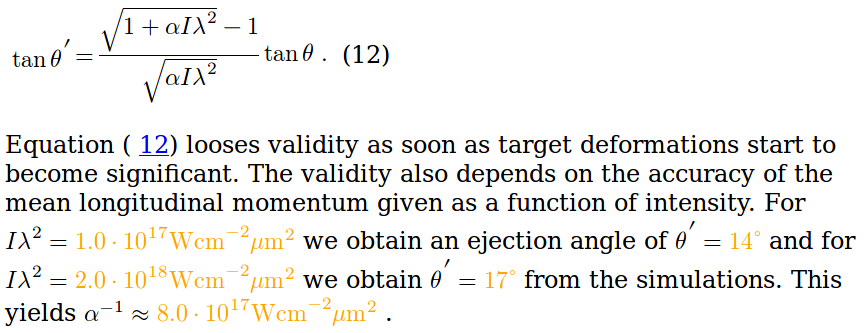
\includegraphics[width=\textwidth]{screenshots/highlight}}
    \caption{Highlighting Quantity Expressions in \cite{physics/9807021}}\label{fig:highlight}
\end{figure}

In the first case, the user wants to convert a unit in just one expression to an equivalent one, say watt to horsepower.
For that, she can right-click on this particular expression and choose a target unit (e.g.  horsepower) from the list of units that are equivalent to Watt.
Figure~\ref{fig:convertone} demonstrates this and Figure~\ref{fig:convertoneresult} displays the result of the computation.

\begin{figure}
  \begin{subfigure}{\textwidth}
    \fbox{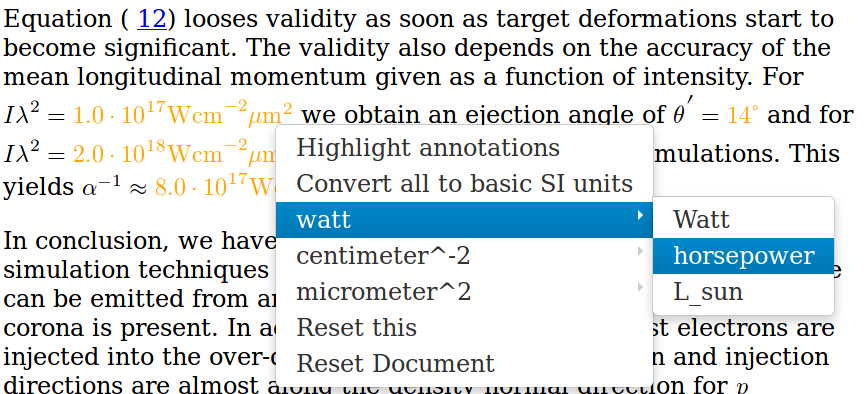
\includegraphics[width=\textwidth]{screenshots/convertone}}
    \caption{Choosing A Target Unit}\label{fig:convertone}
    \fbox{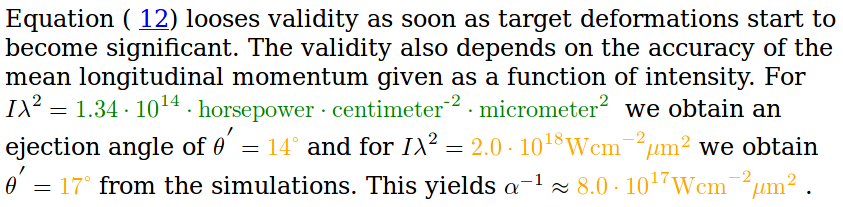
\includegraphics[width=\textwidth]{screenshots/convertoneresult}}
    \caption{The Result of converting one QE}\label{fig:convertoneresult}
    \fbox{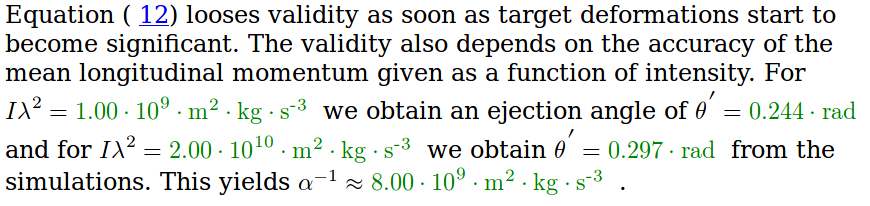
\includegraphics[width=\textwidth]{screenshots/si}}
    \caption{Converting a Document To SI}\label{fig:si}
  \end{subfigure}
  \caption{In-Situ Unit Conversion}\label{fig:unit-conversion}
\end{figure}

The current example only allows local conversions, but of course the user also wants to convert units document-wide -- ideally from one system of measurement to another.
Figure~\ref{fig:si} shows the result of a prototypical implementation, which converts all units to irreducible SI base units.
This could, for instance, be extended to automatically convert all quantity expressions in a document from imperial to metric units and vice versa.

\subsection{A General Framework for In-Situ Computation}\label{sec:impl:general}

In addition to the example above, we have also implemented a prototype of the general in-situ computation manager detailed above.
A right click on a formula $F$ triggers the JOBAD menu, which has an ``Active Computation'' field.

  \begin{itemize}
  \item First, the \textbf{context extractor}, a function that for all the \lstinline|ci| elements in the content formula $C$ associated with $F$, and tries to find the associated variable declarations by going up the parent chain of $F$ and the symbol declarations from the home theory.
  Note that using the content MathML representation $C$ of $F$ gets us around disambiguation problems: even if the presentation of $F$ is ambiguous (e.g. by using variable or constant names multiple times), $C$ is not.
  \item The variable context is displayed to the user prompting instantiation in a popup form: the \textbf{in-situ computation manager} (see Figure~\ref{fig:compman}, which allows to give values for the components of the equation, pick different actions (simplification, equation solving, \ldots ) and ways of providing the results (in-place, footnote, \ldots ).
  As the current system is only a prototype, one can currently only select the Evalutation Action.
  \item In a second step, the  user-supplied values are parsed into content MathML, inserted into $C$, yielding the content MathML expression $C'$, which is then shipped to the computational engine.
  Currently we only support the MMT system as a computational engine, but this is not a restriction, since MMT can delegate computations to engines like GAP, Sage, PARI, \ldots via the SCSCP protocol~\cite{ODK-D3.3}.
  \item Finally, the result $R$ of computing $C'$ -- a content MathML expression -- is inserted back into the original computation context.
  This context can then be presented in presentation MathML and inserted into the document according to the method the user selected \footnote{
  Currently, the system presents the user with the computed context directly. }.
  \end{itemize}

  \begin{figure}[ht]\centering
    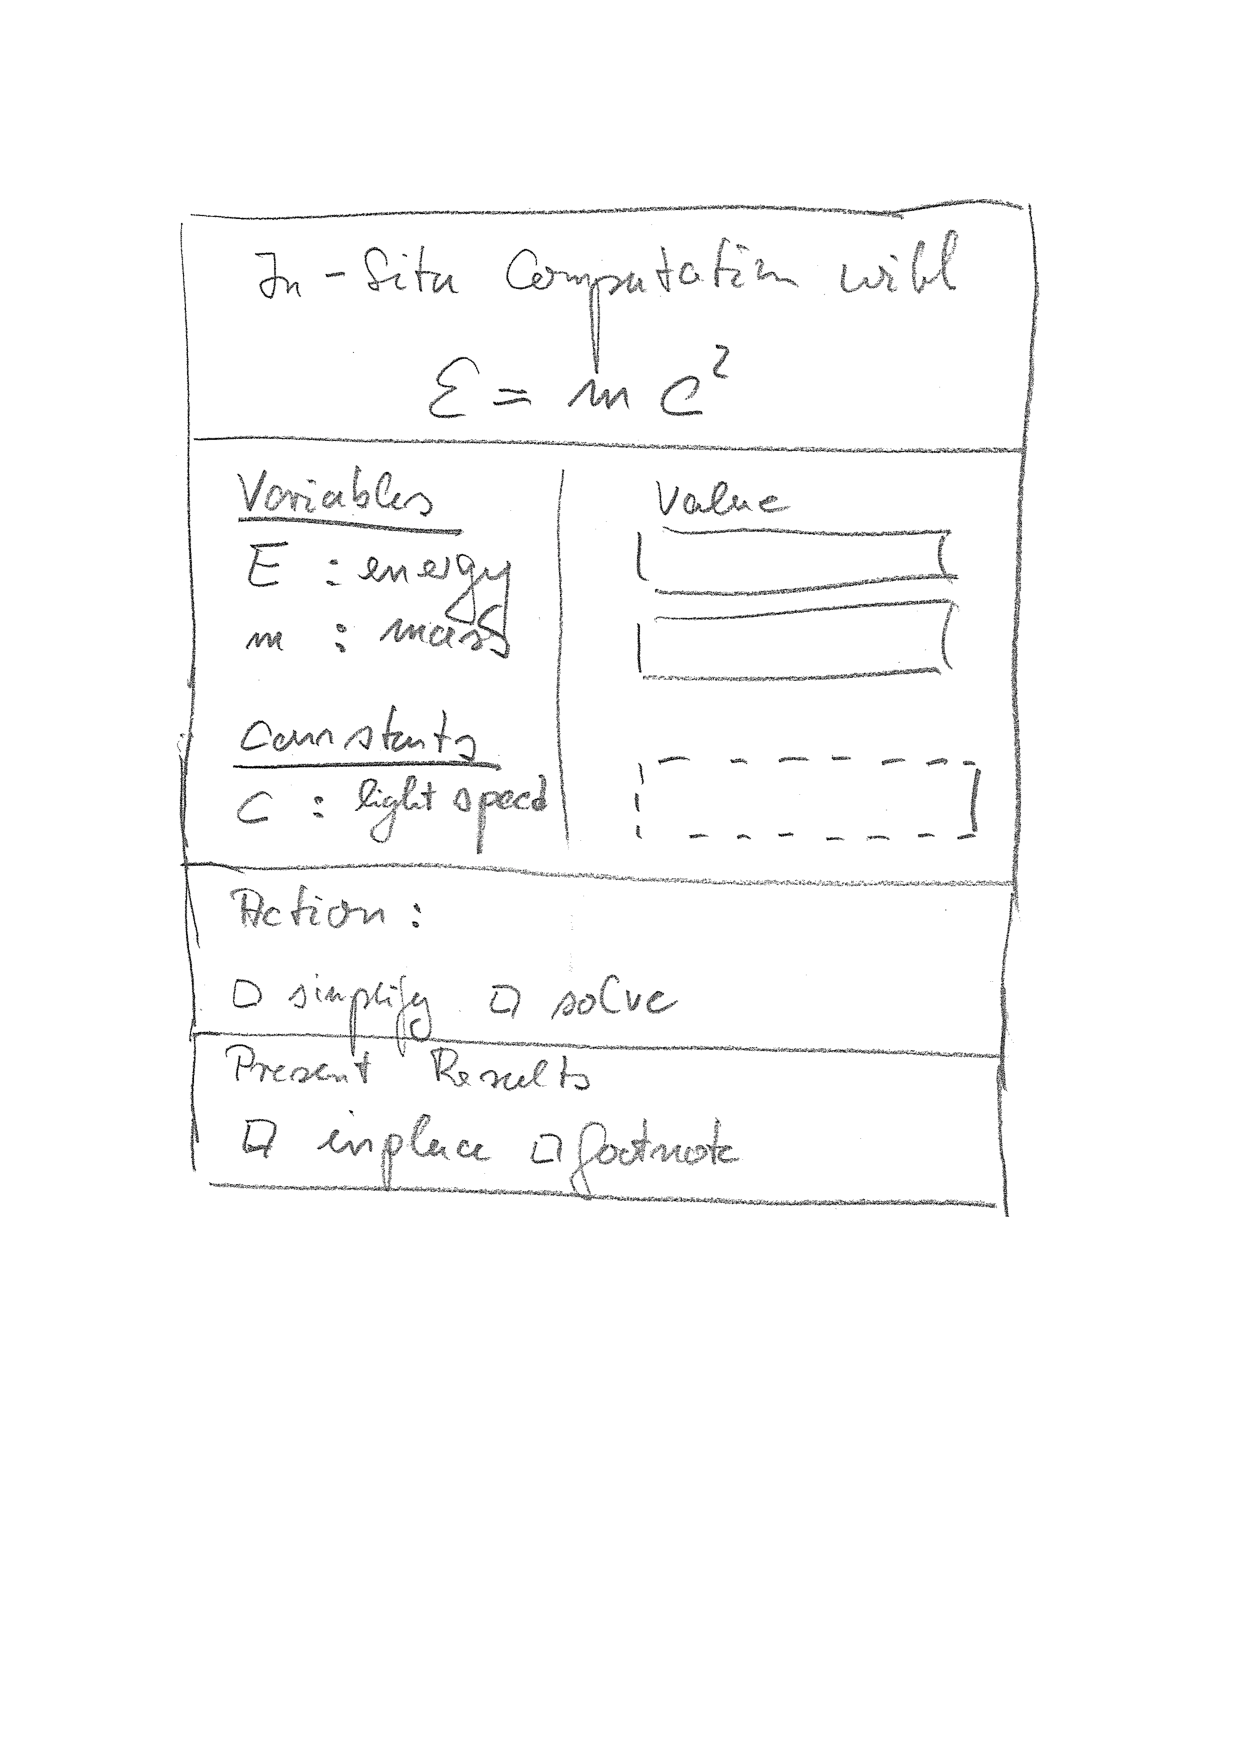
\includegraphics[width=12cm]{screenshots/compman}
    \caption{In-Situ Computation Manager}\label{fig:compman}
  \end{figure}

\subsection{Code Availability, Licensing and Demos}

For both of the examples in this section, an implementation is available under Open Source license terms.
For reasons of lacking MathML support in other browsers, we have only tested these demos in Firefox.

A demo of the unit conversion is available at \url{http://ash.eecs.jacobs-university.de/}.
A user can first select a document and then repeat the procedure detailed above in Section~\ref{sec:impl:units}.
The source code of the demo is available in the repository at \url{https://gl.kwarc.info/urabenstein/Semanticextraction/tree/master/server}.
The server can be executed locally following the steps in the corressponding README file.

A protoype of the General Framework for In-Situ Computation is also availble.
It can be found at \url{http://ash.eecs.jacobs-university.de/prototype/} and shows the basics of the process explained in Section~\ref{sec:impl:general}.
it consists of a frontend component, the source code of which can be found at \url{https://gl.mathhub.info/ODK/ActiveComputationDemo}, as well as a backend component inside the MMT system.
The source code to the backend component can be found at \url{https://github.com/UniFormal/MMT/tree/master/src/mmt-odk/src/info/kwarc/mmt/odk/activecomp}.

%%% Local Variables:
%%% mode: latex
%%% TeX-master: "report"
%%% End:
\newpage
% ---------------------------------------------------------------------------
%  Section 2: Impact
% ---------------------------------------------------------------------------

\TOWRITE{ALL}{Proofread 2 Impact1.4 Ambition pass 2}

\section{Impact}
\label{sec:impact}

%\TOWRITE{Simula}{Hans Petter and Valeriya will make a second iteration on the impact section for Friday}

\TOWRITE{ALL}{Check and complement the impact section}

The project, with its ambitious vision, general and broad approach, and 
challenging work plan, will offer the opportunity to all partners and beyond 
to complement their research expertise with methodologies and tools not 
available at their institutions. It will provide pivotal aspects needed 
for the development of a new generation of high-efficient scientific leaders 
with an open and constructive attitude toward collaborative interdisciplinary 
research and innovation. The diverse nature of the objectives composing the 
project will also be taken into account to design a successful and multiform 
dissemination and exploitation strategy.

\subsection{Expected Impacts}

\eucommentary{Please be specific, and provide only information that applies
to the proposal and its objectives. Wherever possible, use quantified
indicators and targets.\\
Describe how your project will contribute to:\\
-- the expected impacts set out in the work programme, under the relevant topic
(including key performance indicators/metrics for monitoring results and impacts);\\
-- improving innovation capacity and the integration of new knowledge
(strengthening the competitiveness and growth of companies by developing
innovations meeting the needs of European and global markets; and, where
relevant, by delivering such innovations to the markets;\\
-- any other environmental and socially important impacts (if not already
covered above).\\
Describe any barriers/obstacles, and any framework conditions (such as
regulation and standards), that may determine whether and to what extent
the expected impacts will be achieved. (This should not include any risk
factors concerning implementation, as covered in section 3.2.)}

\subsubsection{Impacts as Listed in the Work Programme}

The following Key Performance Indicators (KPI) show how \TheProject  addresses the specific impacts
listed in the work programme. KPIs were thought through by the members
of \TheProject so that they are meaningful, reusable, realistic and easily measurable. The following
qualitative and quantitative indicators are divided into the four aims of \TheProject.
If quantitative indicators are more useful for reporting and internal evaluation, qualitative
indicators will give content for further dissemination and communication purposes,
for example through the project website
\footnote{We will survey mathematical departments
(and relevant members of other departments) 
at the end of each Reporting Period (M18, M36, M48) to gauge the awareness of the 
existence and capabilities of \TheProject and its components, and to collect
statistical data for estimating Key Performance Indicators listed
in the table. The success factor is a positive change between the three surveys.}.

\newenvironment{myaim}[1]
{\noindent{\textbf{#1:}} \begingroup\it}
{\endgroup}

\begin{myaim}{Aim 1}
  Improve the productivity of researchers in pure mathematics and
  applications by promoting collaborations based on mathematical
  software, data, and knowledge.
\end{myaim}

\begin{itemize}
\item Success stories reported as blogposts (Qualitative).
\end{itemize}


\begin{myaim}{Aim 2}
  Make it easy for teams of researchers of any size to set up custom,
  collaborative Virtual Research Environments tailored to their
  specific needs, resources and workflows. The \VREs should support
  the entire life-cycle of computational work in mathematical
  research, from initial exploration to publication, teaching and
  outreach.
\end{myaim}

\begin{itemize}
\item Success stories about \ODK based VRE deployments and
generally speaking adoption of \ODK's components (Qualitative);
\item List of known \ODK based VRE deployments (Quantitative);
\item Number of installs of \ODK's components via platform-specific
  distribution channels: Debian popcon, Arch statistics, installer
  downloads, etc. (Quantitative).
\end{itemize}


\begin{myaim}{Aim 3}
  Identify and promote best practices in computational mathematical
  research including: making results easily reproducible; producing
  reusable and easily accessible software; sharing data in a
  semantically sound way; exploiting and supporting the growing
  ecosystem of computational tools.
\end{myaim}
\begin{itemize}
\item Success stories (Qualitative);
\item Number of PyPI hosted packages for \Sage, and similarly for
  other components (Quantitative);
\item Number of additional systems made interoperable with the
  Math-in-the-Middle architecture, on top of the three for the Month
  36 prototype (Quantitative);
\item Metrics on the scale of the Math-in-the-Middle architecture;
  e.g. number of API CDs generated and number of alignments
  (Quantitative).
\end{itemize}

\begin{myaim}{Aim 4}
  Maximise sustainability and impact in mathematics, neighbouring
  fields, and scientific computing.
\end{myaim}
\begin{itemize}
\item Success stories resulting from dissemination activities such as
  workshops (Qualitative);
\item Statistics on workshops organized and conference presentations
  delivered as part of our dissemination activities, including
  estimates of number of attendees (Quantitative);
\item Number of courses and departments \ODK worked with directly and
  an estimate of how many students this subsequently affected
  (Quantitative).
\end{itemize}

\subsubsection{Improving innovation capacity and the integration of new knowledge}


Innovations developed by the \TheProject project will meet the needs of the
following ecosystem participants:

\begin{compactenum}
\item Device/module vendors: hardware manufacturers, equipment
manufacturers of smartphones, tablets, laptops;
\item Network providers: service providers, network infrastructure
vendors (such as Avaya, Juniper, Extreme, Cisco, et al.);
\item Platform providers;
\item Cloud service providers: Software-as-a-Service,
Platform-as-Service, Infrastructure-as-a-Service;
\item Systeme integrators: end-to-end integration services and
value-added services (such as Accenture, HP, IBM, et al.)
\item End users: research communities; stakeholders in IT, healthcare, 
education, aeronautics, and other areas.
\end{compactenum}
Industrial stakeholders will be directly involved in the project and
the VRE development, so that the tool will be exactly tailored to their
specific needs as well as to the needs of the scientific community.
Moreover, this will allow short time-to-market and will facilitate
the technology uptake.

In the next table we have specified different market needs, and the
ways we will address each of them:

%\begin{flushleft}
\tablehead{}
\begin{longtable}{|m{.30\textwidth}|m{.67\textwidth}|}
\hline
\centering Market needs &
\centering\arraybslash How the project will address these needs\\\hline
Performance gain &
The toolkit will enable its users to combine functionality from several major
open-source mathematical software systems and problem-oriented programming 
languages (including mainstream tools such as Python) in a modern integrated environment) on the majority of currently popular hardware platforms 
and operating systems.
\\\hline
Infrastructure capacity: newly built infrastructures with fast broadband
connections are well positioned for adopting our products &
\TheProject will allow different groups of users to collaborate and work simultaneously on the same document, and
thus providing a considerable gain in efficiency.\\\hline
Low scaling costs &
An open source architecture brings affordability: people and
organisations donate efforts towards common goals, and small organisations can
gain access to equipment and research talents otherwise only affordable by
the largest companies. Resources integration will reduce considerably the
time and the costs of operations.\\\hline
Going beyond limitations of interconnect technology &
An open source architecture enhances creativity due to the potential to
attract best minds from a wide pool of people to solve a problem\\\hline
Enabling new applications and features &
Through a series of connections that will be created between previously
separated tools, and data interoperability, \TheProject will enable new
applications and features. All derived VREs are new applications, with new features.\\\hline
Early time-to-market (TTM): companies are looking for solutions that
would improve the speed at which they can procure services to bypass
traditional information technology departments &
The speed of development will improve tremendously due to the new
collaborative features. Liaising with industrial stakeholders during
the development will allow to deliver a tool the suits their needs in
the best possible way, thus speeding-up the time-to-market and technology 
uptake.\\\hline
Easy-to-use service: first-time experiences are crucial to gain
acceptance &
We will design an ergonomic multi-user web-based graphical user
interface, following web standards to best support a large array of
browsers, including cell phones and tablets. We will explore
opportunities for integration in interactive boards, as an aid for
teaching and collaborative research.
\\\hline
\end{longtable}
%\end{flushleft}

\subsubsection{Other Impacts (Environmental and Socially Important Impacts)}


We start from \Sage's mission statement: ``Creating a viable free open
source alternative to \Magma, \Maple, \Mathematica and \Matlab'' but
need to go beyond that goal, and make \TheProject a new reference
tool, that is deployed across science. To be successful our VREs will
need to provide much more than can be done through closed source
commercial systems. Large scale collaborative development is the key
to this goal, both on software and research, but coordination and
projection of vision is still crucial for success. We will focus on
the young generation, which will constitute its future users, for
example by producing learning materials for the so called ``Generation
Y''. ``Generation Y'' is expected to account for 30\% of the total
projected population in 2025, and will be the key influencer for
change in workplace habits, caused by such features as easy
adaptability to new technologies and social media, commonly attributed
to this generation.  \TOWRITE{??}{May we add some reference to support
  this statement?}

\TOWRITE{AK}{This section needs to be extended} 

\subsubsection{Potential Barriers to Impact}

The following barriers to impact will be addressed and overcome using the mitigation
strategies provided. These are distinct from the risks to project delivery
detailed in Section~\ref{sec:risks}.
\TOWRITE{ALL}{Some other barriers? Maybe lack of contribution from community to OpenDreamKit?}
\paragraph{Table 2.1: Barriers to Impact}
\begin{longtable}{ | p{10cm} | c | }\hline
{\bf Barrier description } & {\bf Risk level }\\\hline \hline
{\bf Users will not use the new VRE environment}       &  High       \\\hline
\multicolumn{2}{| p{.97\textwidth}|}{
{\bf Contingency Plan:}  
A major concern in any proposal of this kind is that the resulting
tools will not be adopted by users. This is a particular concern with
such 'tradition-based' community as mathematicians.  This project has two pathways to tackle this:
(1) \TheProject is based on prior work, which \emph{already} has users;
(2) \TheProject will be integrated into the \Jupyter and \Sage, which \emph{already} have a significant user base;
(3) An end-user group formed at the beginning of the project by the representatives from different disciplines and sectors will provide valuable advice on real user needs throughout the project and assist in providing \TheProject sustainability.

In addition, the project's communication, dissemination, and
exploitation strategy will evolve throughout the project's implementation to
ensure that stakeholder communities are fully aware of the project's
progress, potential benefits, and innovative capacity and are engaged
in the integration of the final results.
}\\\hline
{\bf Dominance of competing frameworks  }  &  Medium        \\\hline 
 \multicolumn{2}{| p{.97\textwidth}|}{
{\bf Contingency plan:}  
  Our strategy is to engage with  users  and attract new users at the very beginning
of the project, understand their requirements and design the domain-specific tools.
An international advisory
board will allow us to coordinate with the related research activities within and outside of Europe
and to promote our framework internationally.}\\\hline
\end{longtable}
\TOWRITE{All and NT}{Is dominance of competing frameworks really an issue? Is there anything out there AS GOOD as OpenDreamKit? Would be good to have more than just one barrier though.}



\subsection{Measures to Maximise Impact}
\TOWRITE{ALL}{go through the section and add specific input, relevant to your organisation on dissemination / exploitation activities}
The overall objectives of the dissemination and exploitation strategy are based on the project's core values, which are to improve the productivity of researchers in mathematics and connected fields by providing them with a unique virtual toolkit for a collaborative research tailored to their needs and requirements both during the project period and after the project completion.

\subsubsection{Dissemination and Exploitation of Results}
\label{subsubsect:dissemination}
\eucommentary{-- Provide a draft 'plan for the dissemination and exploitation
of the project's results'. The plan, which should be proportionate to the
scale of the project, should contain measures to be implemented both during
and after the project.\\
Dissemination and exploitation measures should address the full range
of potential users and uses including research, commercial, investment,
social, environmental, policy making, setting standards, skills and
educational training.\\
The approach to innovation should be as comprehensive as possible,
and must be tailored to the specific technical, market and organisational
issues to be addressed\\
-- Explain how the proposed measures will help to achieve the expected impact of the
project . Provide a draft business plan for financial sustainability as stated in the Part
E of the Specific features for Research Infrastructures of the Horizon 2020 European
Research Infrastructures (including e-Infrastructures) Work Programme 2014-2015.\\
-- Where relevant, include information on how the participants will
manage the research data generated and/or collected during the
project, in particular addressing the following issues:
What types of data will the project generate/collect? What
standards will be used? How will this data be exploited and/or
shared/made accessible for verification and re-use (If data cannot
be made available, explain why)? How will this data be curated and preserved?\\
-- Include information about any open source software used or developed by the
project.\\
You will need an appropriate consortium agreement to manage (amongst other things)
the ownership and access to key knowledge (IPR, data etc.). Where relevant,
these will allow you, collectively and individually, to pursue market opportunities
arising from the project's results.\\
The appropriate structure of the consortium to support exploitation is addressed
in section 3.3. \\
-- Outline the strategy for knowledge management and protection. Include measures to
provide open access (free on-line access, such as the ``green'' or ``gold'' model) to
peer-reviewed scientific publications which might result from the project.\\
Open access publishing (also called 'gold' open access) means that an article is
immediately provided in open access mode by the scientific publisher. The associated costs
are usually shifted away from readers, and instead (for example) to the university or
research institute to which the researcher is affiliated, or to the funding agency supporting
the research.\\
Self-archiving (also called ``green'' open access) means that the published article or the
final peer-reviewed manuscript is archived by the researcher - or a representative - in an
online repository before, after or alongside its publication. Access to this article is often -
but not necessarily - delayed (``embargo period''), as some scientific publishers may wish to
recoup their investment by selling subscriptions and charging pay-per-download/view fees
during an exclusivity period.}


The dissemination and exploitation strategy will be
presented in the dissemination and exploitation plan, prepared by the
Coordinator within \TOWRITE{All}{Add reference to task that produces
  dissemination and exploitation plan} the specifically designed WP
and implemented with the help of all partners. The planned activities
will bear in mind the project's scientific and societal impacts, and
build throughout the project to ensure that stakeholder communities
(1) are fully aware of the project and its potential benefits, (2)
engaged in integration of the VRE in their professional activities,
and (3) contribute to the sustainability and improvement of the
VRE. 

We summarise the dissemination activities
and how they will help to achieve the expected impact among our
stakeholders and target audiences in Table~\ref{table:dissem-plan}.

%% HF got to here reviewing 

%Three types of impact are possible with our dissemination and
%communication activities: (1) people or organizations are informed
%about \TheProject; (2) people or organizations act and use our conclusions
%or results; (3) people or organizations contribute and help to develop
%or improve the research infrastructure. The second form of impact
%supposes that parties understand the messages. The third form supposes
%learning, which is a very high level of impact. In the following table,
%we have listed how the proposed measures will help to achieve the
%expected impact among our stakeholders and target audiences.

\begin{table}
\begin{longtable}{|m{3cm}|m{1cm}| m{.56\textwidth} | m{2cm}|}\hline
Dissemination goal &
Target audience&
Dissemination method &
Timeframe and frequency  \\\hline
Project identity and profile &
T1-T6
&
Website; flyers/leaflets; videos.
& 
Throughout project, continuous \\\hline
Broad dissemination &
T3, T4, T6, T7 
&
Biannual e-newsletters; press releases; information database; social networks and platforms; news  in Nature and other editions in other disciplines; lectures in high schools led by PhD students.
& 
Throughout project, quarterly \\\hline
Knowledge transfer, information exchange&
T1,T2, T3
&

Organisation of 10 technical workshops; 10 scientific trainings/year; training of at least 100 PhD students for the infrastructure usage; publications in social aspects; software demonstration during conferences; workshop for PhD students in Africa; participation at the workshop 'Sage and women' in US; participation in international conferences like FPSAC, ISSAC, or the international congress of mathematical software; regular participation in annual Python conference; organising at least 8 scientific trainings for other scientific communities/projects; news  in Nature and other editions in other disciplines; certification by technology clusters.
& 
Throughout project, continuous  \\\hline
Demonstration of advantages and possible applications &
T1-T4
&
Organisation of 10 technical workshops; participation in annual Python conference.
& 
Biannually \\\hline
Uptake of the VRE by new users &
T2-T4
&
White papers; organise at least 8 scientific trainings for other scientific communities/projects; presentation at international conferences; 5 MooCs designed to master students; integration of project results into Master courses and into teacher training courses.
& 
Mo24-, at relevant milestones \\\hline
Sustainable development beyond the project &
T1-T4
&
Policy events; white papers; participation at conferences.
& 
Mo24-, at relevant milestones \\\hline
\end{longtable}

\smallskip
{\bf Key for the ``Target Audience'' column:}
\begin{compactenum}
\item[T1] Scientific community in mathematics and related fields 
     (experienced researchers, under-/graduate/post-graduate students);
\item[T2] Scientific community in other disciplines;
\item[T3] Other relevant European and national initiatives and projects;
\item[T4] Industrial end-users;
\item[T5] Standardisation agencies;
\item[T6] Civil society;
\item[T7] Public at large.
\end{compactenum}
\caption{\label{table:dissem-plan}Dissemination and exploitation plan}
\end{table}

%
%\begin{flushleft}
%\tablehead{}
%\begin{longtable}{|m{2cm}|m{8cm}|l|l|l|}
%\hline
%
%Target users &
%Measures during the project &
%\multicolumn{3}{m{3.9129999cm}|}{Expected impact}\\\hline
% &
% &
%(1) &
%(2) &
%(3)\\\hline
%Scientific community in mathematics
%
%(experienced researchers and PhD students) &
%\begin{compactenum}
%\item Recruitment for the project of specialists from industrial sector
%and PhD students that are already a part of the community ;\item 10
%technical workshops organised in the frame of \TheProject, \item 10
%publications in (social aspects) \item Software demonstration during
%the conferences{\textgreater}publication\item 100 PhD students trained
%and accessing the infrastructure\item Workshops for PhD students in
%Africa
%\end{compactenum}
% &
%X
%
%X
%
%X
%
%X &
%X
%
%X
%
%X
%
%X
%
%X
%
%X
%
%X &
%X
%
%X
%
%X
%
%X
%
%X
%
%X\\\hline
%Scientific community in other disciplines &
%\begin{compactenum}
%\item Direct implication of the representatives of those disciplines
%into the project;\item Annual participation in Pycon international
%conference\item X scientific trainings to other communities; \item News
%in Nature and other editions in other disciplines (specify!)\item Up to
%X PhD students trained on the tool in biology, physics etc.\item
%Workshop ``~sage \& women~'' in USA{\textgreater} pour
%IPython
%\end{compactenum}
% &
%X
% &
%X
%X
%X
%X
%X
%X
% &
%X
%X
%X\\\hline
%Policy makers &
%Are not directly concerned by the tool, but can be informed via
%international conferences and publications &
%X &
% &
%\\\hline
%Industry &
%\begin{compactenum}
%\item Industrial stakeholders have common needs with academic
%researchers. They bring to the project their specific competences and
%human resources. They are actively involved into the workshops and
%trainings (50\% of audience). The project aims the enlargement of the
%community thanks notably to new industrial actors (including in other
%disciplines and sectors). They will appropriate the tool by their
%direct involvement into the project, by participation to the workshops,
%trainings and conferences or by their usual information channels.\item
%Annual participation in Pycon international conference\item
%Certification by technology clusters
%\end{compactenum}
% &
%X &
%X
%X
%X
% &
%X\\\hline
%Standartisation
%
%agencies  &
%\begin{compactenum}
%\item At the end of the project,~after internal standartisation, the new
%norms will be accorded with specialised agencies at national and EU
%levels
%\end{compactenum}
% &
% &
%X &
%\\\hline
%Students &
%\begin{compactenum}
%\item 5 MooCs destined to master students.\item The tool will be used
%for the elaboration of pedagogical documents, referenced on the
%specific website\item The projects results will be integrated into
%Master courses, and into teacher training courses
%\end{compactenum}
% &
%X
%X
%X
% &
%X
%X &
%\\\hline
%Civil society &
%\begin{compactenum}
%\item Results will be presented on the annual event “Worldwide meetings
%of the free software”. This event generally touches upon all free
%phenomena in the society, and involved various stakeholders, including
%civil society actors.
%\end{compactenum}
% &
%X &
%X &
%\\\hline
%Public at large &
%\begin{compactenum}
%\item Series of actions in high schools led by PhD students to raise
%awareness of pupils, and especially girls, on mathematics research and
%scientific careers\item Communication large public via annual events
%like ``~Science holiday~'' etc.\item Vulgarization papers and
%communication events addressed to people interested by ICT. \item Social
%networks and platforms
%\end{compactenum}
% &
%X
%X
%X
%X &
% &
%\\\hline
%\end{longtable}
%\end{flushleft}

{\bf Post-project Activities:} The natural interest of the consortium is to ensure sustainability of \TheProject also after the completion of the project. Therefore, the partners are committed to post-project efforts, which include the following activities: 
\begin{compactenum}
\item Continue dissemination to scientific community and industrial stakeholders through participation to international conferences (FPSAC, ISSAC, Python, \Sage and Women etc.) and publications.
\item Software demonstration during the conferences.
\item Training of  PhD students in mathematics, informatics and other disciplines, both in Europe and all over the world. Gradual incorporation of \TheProject components into the relevant university courses beyond \TheProject members home institutions.
\item Expand \TheProject user base by continuing the research collaboration with existing users and  identifying new scientific (specifically from neighbouring fields) and industrial users.
\item Apply for funding at European / national levels for new projects that are to improve and further promote \TheProject.
\end{compactenum}

\TOWRITE{ALL}{Please give a look at general exploitation and provide input relevant to your interests / interest of your organisation. In particular, possible commercial exploitation.}

{\bf Exploitation:} To exploit and capitalise on the success of the project, we will undertake the following activities
\begin{compactenum}
\item Engaging stakeholders and potential users of \TheProject in Europe for realising the technology transfer and the innovation potential of the toolkit;
\item Teaching the \TheProject-induced research results as parts of relevant courses at university, which are the home institutions of the consortium members, as well as at the on-going training events and activities);
\item Mentoring and training PhD and postdoctoral students within the project as our contribution to educating excellent interdisciplinary European researchers in the strategically important domain of natural sciences;
\item Applying for European / other relevant funding programmes for new projects which arise due to the maturity of the \TheProject;
\item Supporting spin-offs based on the developed technology by the consortium partners. In this case, the IPR management will be aligned with the corresponding rules set in the Consortium Agreement.
\end{compactenum}

\TOWRITE{NT}{Prepare a proper description of a business plan}

Draft business plan for financial sustainability (as stated in the Part
E of the Specific features for Research Infrastructures of the Horizon
2020 European Research Infrastructures (including e-Infrastructures)
Work Programme 2014-2015).

\paragraph{Long term sustainability}

By design (Objective~\ref{objective:framework}), the VREs promoted by
\TheProject will consist of a thin layer on top of an ecosystem of open source
components. Hence, the long term
sustainability of those VREs is guaranteed by the sustainability of the
ecosystem of components (Objective~\ref{objective:sustainable}).

By the end of the project, we expect that the main barriers will have
been addressed, and that the needs for financial support will
therefore not be very important. Furthermore, we expect that some of
developers' positions will be extended beyond the duration of the project 
by the partners' institutions, due to the increase of awareness among them 
on the necessity of this infrastructure for their own needs.

With the increase of the number of users, more and more research
laboratories, teaching institutions, and companies will desire to
use and further improve and benefit from \TheProject VREs or components
thereof. This will lead to further feedback and improvements, and also
will open the door for the attracting additional funding, either:
\begin{itemize}
\item through access provision to other scientific communities, on
  projects base, or via service delivery; this opportunity is for
  example already being explored by the \SMC project in the US: it
  recently spun off a company on this business model to seek for
  additional funding.
\item through specific developments and training services delivered by
  companies like \site{LL} that have a solid business model based on
  open source software.
\end{itemize}

We conclude by a quote of Stéphane Fermigier, president of the Open
Source Software Working Group\footnote{\url{http://www.systematic-paris-region.org/en/get-info-topics/free-and-open-source-software}}
of the Systematic Paris Region Systems \& ICT Cluster (having
\site{PS} and \site{LL} as members),
and founder of NUXEO\footnote{http://www.nuxeo.com/}:
\begin{quote}
  Open source is still reshaping all aspects of the software industry,
  specially high growth sectors such as Big Data, Enterprise 2.0 or
  Mobile Applications. NOT using open source components is now
  considered the exception rather than the rule in almost all
  companies that produce software, creating a tremendous opportunity
  for the Paris Region open source ecosystem, whose leadership has
  been recognised for a long time, from academic research teams to
  young innovative software vendors, from specialised consultancies to
  large systems integrators.
\end{quote}

%As showcased by the success of the Logilab company (\site{LL})
%Other models, are mo

% \TODO{None of the two models below really match our situation;
%   investigate for some good picture and language, e.g. in ``Economie
%   du Logiciel Libre'' of François Élie}

% Here we propose two possible models of this use:

% \begin{figure}[ht]\centering
%  \fbox{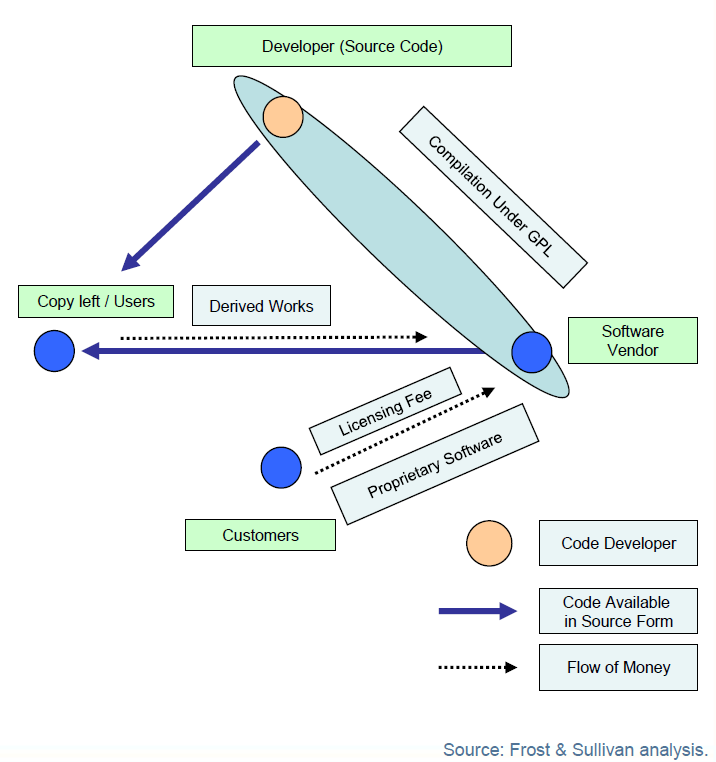
\includegraphics[width=.94\textwidth]{Impact-img1.png}}
%  \caption{The GPL Model}\label{fig:gpl-model}
% \end{figure}

% \begin{figure}[ht]\centering
%  \fbox{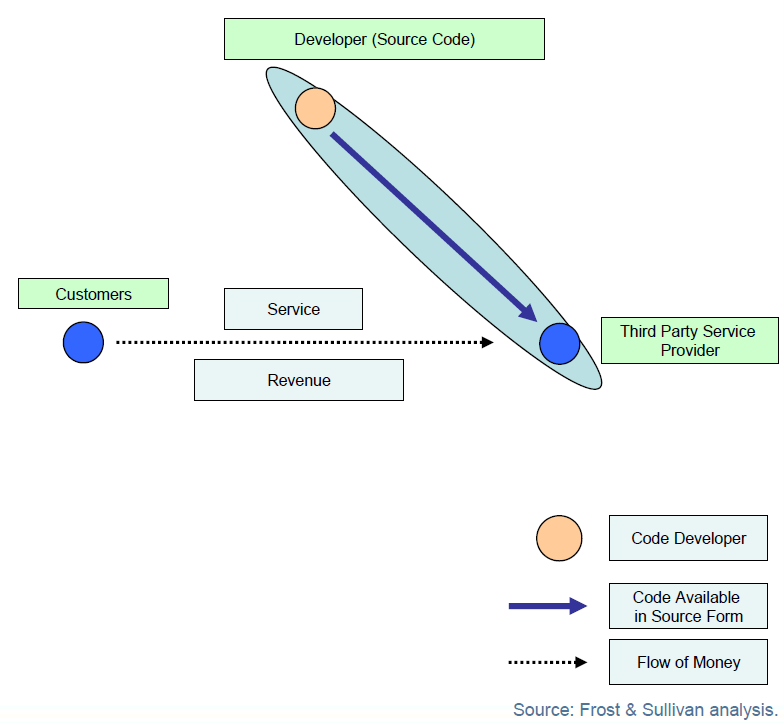
\includegraphics[width=.94\textwidth]{Impact-img2.png}}
%  \caption{The Third-Party Services Model}\label{fig:tps-model}
% \end{figure}

% \begin{compactenum}
% \item The \textbf{GPL model} (see Figure~\ref{fig:gpl-model}): With this model, the vendor
%   is required to make the new code available in source form but it can choose to keep the
%   new code as proprietary and charge for that proprietary software.  The vendor can
%   provide the code commercially as part of a larger platform (hardware/software product)
%   for which the companies receives revenue (license fee for the code + fees for technical
%   support, updates and upgrades).
% \item The \textbf{Third Party Service Model} (see Figure~\ref{fig:tps-model}) Many users
%   may be willing to employ a third party service for distribution, modifications
%   (debugging) and other support.
% \end{compactenum}

\eucommentary{
Where relevant, include information on how the participants will manage
the research data generated and/or collected during the project, in
particular addressing the following issues: What types of data will the
project generate/-collect? What standards will be used? How will this
data be exploited and/or shared/made accessible for verification and
re-use (If data cannot be made available, explain why)? How will this
data be curated and preserved?}

\TOWRITE{E.S. – Nicolas}{, ici je ne peux pas  écrire à ta place. Il faut juste que
tu répondes précisément aux questions posées ci-dessus.}

%Open source software.
%
%
%All software used and/or generated by the project will be Open Source.
%This is a deliberate choice of the project consortium, as commercial
%licenses (and patents) on this type of software only creates barriers
%in our scientific domain.
%
%Benefits of Open Source:
%
%Acquisition and Costs: lower costs, easy access to the infrastructure,
%lower risks of proprietary lock-in
%
%Flexibility: picking up from Open Source projects, reduces dependence on
%supplier, ability to view and modify the source code. Allows peer
%reviewed modifications, community discussions. Open Source provides the
%customer/end user the opportunity to innovate
%
%Support: from developer community.
%
%Besides being cost effective, Open Source software fosters
%reuse, reliability, flexibility, and interoperability.
%
%A consortium agreement will be established to manage ownership and
%access to key knowledge, including software generated by the project.

{\bf Open access policy and data protection.} OpenDreamKit will participate in the Open Research Data Pilot and is fully committed to ensure the open access of relevant project results and data. The consortium will comply with the Guidelines on Open Access to Scientific Publications and Research Data in Horizon 2020. 

The ambitious and interdisciplinary objectives of the project will result in the production of vast amount of research data (we refer to Figure \ref{fig:thebigpicture} and the corresponding subsection for more details). The primary results of the project are expected to take the form of an open-source software, which will be available through the project website and publicly available repositories. Moreover, as the project strives towards efficient integration and representation of various research data and reproducibility of the research results, which represents naturally a challenge, the project will generate a detailed description of the data sources with specifics pertaining to data management (metadata standards, policies for access and sharing and for reuse and distribution, plans for archival and preservation, with accompanying deadlines). This information will be presented in the Data Management Plan, to be delivered within the first six months after the project start and subsequently updated throughout. 

All scientific publications produced in the framework of the project will be either published in open access journals or self-archived using research data repositories. In addition, we will make all experimental data needed to reproduce/validate the results from scientific publications available through research data repositories (e.g. ZENODO, OpenAIRE). 

{\bf Intellectual Property Rights Management.} IPR management will be described in detail in the Consortium Agreement (CA), which will describe all issues regarding the IPR, confidentiality, know-how, rights on exploitation, the rights and obligations of the each partner. The CA will be prepared by the Coordinator, and then signed by all partners before the start of the project. 

Access rights to foreground and background needed for the execution of the project shall be deemed granted, on a royalty-free basis, as of the date of the grant agreement entering into force. Methodology, documents, know-how, software, and tools will be available to all in order to achieve the project objectives during the project lifetime. 

Most of the project results will have joint ownership due to a highly collaborative nature of the project. The CA will specify the terms of the resulting joint ownership, i.e., assignment of shares between joint owners, conditions of use, exploitation and management of jointly used IP. 

The CA will also outline rules for publication procedures to ensure that IP can be protected while minimising publication delay.

The costs related to IPR (including those related to protecting results) and dissemination (i.e., 'gold' open access publications) are included in the project budget of each participating organisation. 

\subsubsection{Communication Activities}
\label{subsubsect:communication}

\eucommentary{Describe the proposed communication measures for promoting the
project and its findings during the period of the grant. Where appropriate
these measures should include social media and public events with user
participation. Measures should be proportionate to the scale of the project,
with clear objectives. They should be tailored to the needs of various audiences,
including groups beyond the project's own community. Where relevant, include
measures for public/societal engagement on issues related to the project.}

Our intention is to increase the attractiveness of mathematics among young generation and females in particular as well as to improve the impact and maximise the visibility of the project activities on the entire VRE ecosystem. The following strategic access points will be used to maximise visibility:

\begin{compactenum}
\item An online presence that explains the OpenDreamKit concept and its applicability in layman's terms and offers significant information (website, social networks, Youtube, press releases).
\item Collaboration with other relevant European and national projects (existing and new ones). We refer to Section \ref{linked-projects} for more details on the linked research and innovation activities.  Presentation of the project results on the annual event 'Worldwide meetings of the free software.' 
\item Collaboration with European and national mathematical societies, e.g., European Mathematical Society, European Women in Mathematics.
\item Presentations/demonstrations at partner institution-specific, locally organised 'science holiday' and 'days of science'.
\item Popularisation papers and communication events addressed to people interested by ICT. 
\item Involvement in workshops / conferences on e-infrastructures and broad mathematical topics, e.g., Swiss Numerical Analysis Day.
\end{compactenum}
%%% Local Variables:
%%% mode: latex
%%% TeX-master: "proposal"
%%% End:

%  LocalWords:  eucommentary programme subsubsection tablehead longtable hline sur est
%  LocalWords:  e-infrastracture sémantique données amont j'ai mal si répond vraiment ce
%  LocalWords:  critère Systeme flushleft arraybslash Ergonomie il faut réflechir façon
%  LocalWords:  rendre l'outil attractif jeune génération génération des chercheurs va je
%  LocalWords:  définir donc terme Réfléchis possibilité tablettes mais aussi l'enseigner
%  LocalWords:  intéressante textgreater partie suivante demande elle ne serait mieux que
%  LocalWords:  unauthorised Maximise subsubsect organisational Pycon IPython Economie tu
%  LocalWords:  Standartisation Logiciel Libre includegraphics Impact-img1.png peux emph
%  LocalWords:  Impact-img2.png écrire répondes précisément posées ci-dessus TOWRITE fbox
%  LocalWords:  Simula Valeriya textwidth textwidth textbf compactenum longtable Jupyter
%  LocalWords:  organisation organise neighbouring Standartization programmes gpl-model
%  LocalWords:  tps-model thebigpicture Popularisation virtualised organisations Logilab
%  LocalWords:  organisations summarise organising capitalise realising minimising
%  LocalWords:  organised
\newpage
\end{proposal}
\TOWRITE{ALL}{Proofread 4. Members of the consortium pass 2}

\subsection{Participants}

\eucommentary{Please provide, for each participant, the following (if available):\\
\begin{compactitem}
\item
a description of the legal entity and its main tasks,
with an explanation of how its profile matches the tasks in the proposal;
\item
a curriculum vitae or description of the profile of the persons,
including their gender, who will be primarily responsible for carrying
out the proposed research and/or innovation activities;
%
this includes a description of the profile of the to-be-recruited personnel
\item
a list of up to 5 relevant publications, and/or products, services
(including widely-used datasets or software), or other achievements
relevant to the call content;
\item
a list of up to 5 relevant previous projects or activities, connected
to the subject of this proposal;
\item
a description of any significant infrastructure and/or any major items
of technical equipment, relevant to the proposed work;
\item
any other supporting documents specified in the work programme for this call.
\end{compactitem}}

\begin{sitedescription}{PS} \label{desc:ParisSud}

The Université Paris-Sud is among the 40 top universities worldwide in the
2013 Shanghai ranking, and is one of the two best French research
universities. With about 27000 students, 1800 permanent teaching staff
and 1300 permanent research scientists from national research
organisations (CNRS, Inserm, INRA, Inria), it is the largest campus in
France. Since 2006, scientists from the University were awarded two
Fields medals, one Nobel Prize and a number of other national and international
(European Inventor Award 2013, Wolf Prize 2010, Holweck Prize 2009,
Japan prize 2007) prizes.  The Université Paris-Sud offers a
complete range of qualifications, ranging from the purest of exact
sciences to clinical practices in medicine, covering life and health
sciences, legal sciences and economics. Research at the Université
Paris-Sud, an essential part of academic understanding, is
complemented by research activities with a high commercialisation
potential. Research contracts and partnership with companies make the
Université Paris-Sud a key actor and a major player in French
research.  The Université is located close to the Plateau de Saclay,
the largest cluster of public and private R\&D institutions in France
(with ca. 16000 research staff), and is one of the core members of the
University Paris Saclay – a world class university and a
world-renowned research and innovation hub.

In the context of this project, the Université Paris-Sud is the
home of one of the largest group of \Sage developers worldwide.
It's a member of the Open Source Thematic Group of the Systematic
Paris Region Systems and ICT Cluster. The University also hosts a
major research group (VALS) working on proof assistants (\software{Coq}) and
another on Human Centered Computing, which will facilitate reaching
toward those communities.

The Université Paris-Sud will lead the project (\WPref{management}),
host the majority of the man power for \WPref{component-architecture}
Component Architecture, and lead or contribute to tasks on or around the \Sage
computational system (\taskref{component-architecture}{extract-smc},
\taskref{component-architecture}{interface-systems},
\taskref{UI}{ipython-kernels}, \taskref{UI}{sage-sphinx},
\taskref{UI}{dynamic-inspect}, \taskref{hpc}{hpc-combi},
\taskref{dksbases}{data-memo}). Finally, it will lead \WPref{dissem} and in
particular host or coorganise many of the community building,
training, and dissemination actions.

% The main participants have accumulated 15 years of experience of
% collaborative open source software development for mathematics
% leadership, and community animation.

\subsubsection*{Curriculum vitae of the investigators}

\begin{participant}[type=leadPI,PM=5,gender=female]{Viviane Pons}
  Maître de Conférences at the Laboratoire de Recherche en Informatique, Viviane Pons is a
  young researcher in Algebraic Combinatorics. She defended her thesis in 2013 and has 3
  papers in international journals and 3 communications in international
  conferences, including a talk at PyCon US 2015. Before starting research career, 
  she worked for two years in industry as a Java and web developer.

  She discovered \Sage during her first \Sage Days in 2010 and has since been an active user
  and contributor with 10 (co)authored tickets improving the support of combinatorial
  objects in \Sage. She is heavily involved in the promotion of \Sage, participating in
  \Sage Days and running \Sage introduction tutorials or \Sage presentations at various
  conferences. She is also one of the main developers of the project \software{FindStat}
  dedicated to databases in combinatorics.
\end{participant}
%%% Local Variables:
%%% mode: latex
%%% TeX-master: "../proposal"
%%% End:

%\input{CVs/Nathann.Cohen}
\begin{participant}[type=PI,PM=5,gender=male]{Florent Hivert}

  Professor at the Laboratoire de Recherche en Informatique, Florent Hivert is a senior
  researcher in Algebraic Combinatorics with 29 papers in international journals and 15
  communications in international conferences.
% including an invited lecture at FPSAC'10

With 100 \Sage tickets (co)authored and as many refereed, Hivert is himself a core \Sage
developer, with contributions including key components of the \Sage infrastructure
(documentation, automated test, combinatorics infrastructure, parallelism, \ldots)
and specialised research libraries.
\end{participant}
%%% Local Variables:
%%% mode: latex
%%% TeX-master: "../proposal"
%%% End:

\begin{participant}[type=PI,PM=12,gender=male]{Nicolas M. Thiéry}
  Professor at the Laboratoire de Recherche en Informatique, Nicolas M. Thiéry is a senior
  researcher in Algebraic Combinatorics with 15 papers published in international
  journals. Among other things, he is a member of the permanent committee of FPSAC, the
  main international conference of the domain, and has collaborators in Canada, India, and
  in the US where he spent three years (Colorado School of Mines, UC Davis). He also
  co-organised fourteen international workshops, in particular \Sage Days, and the semester
  long program on ``Automorphic Forms, Combinatorial Representation Theory and Multiple
  Dirichlet Series'' hosted in Providence (RI, USA) by the Institute for Computational and
  Experimental Research in Mathematics.

  Algebraic combinatorics is a field at the frontier between mathematics and computer
  science, with heavy needs for computer exploration. Pioneer in community-developed open
  source software for research in this field, Thiéry founded in 2000 the \SageCombinat
  software project (incarnated as \MuPADCombinat until 2008); with 50 researchers 
  in Europe and abroad, this project has grown under
  his leadership to be one of the largest organised community of Sage developers, gaining
  a leading position in its field, and making a major impact on one hundred
  publications\footnote{\url{http://sagemath.org/library-publications-combinat.html},
    \url{http://sagemath.org/library-publications-mupad.html}}. Along the way,
%this occasion
%Thiéry gained a strong community building experience, and
  he coauthored part of the proposal for NSF \SageCombinat grant
  OCI-1147247, and co-organised or taught at a dozen training and
  dissemination actions (workshops, summer schools, etc.), in
  America, Africa, Europe and India.

  With 150 tickets (co)authored and as many refereed, Thiéry is himself a core \Sage
  developer, with contributions including key components of the \Sage infrastructure
  (e.g. categories), specialised research libraries (e.g. root systems), thematic
  tutorials, and two chapters of the book ``Calcul Mathématique avec \Sage''.
\end{participant}
%%% Local Variables:
%%% mode: latex
%%% TeX-master: "../proposal"
%%% End:

\begin{participant}[type=R,PM=5,gender=male]{Samuel Lelièvre}
Maître de conférences since 2006 at
Laboratoire de mathématique d'Orsay, Université Paris-Sud,
% PhD Rennes 2004 under Anton Zorich,
% post-doc Warwick with Vladimir Markovic,
Samuel Lelièvre is an established researcher in Dynamics and Geometry,
with 10 papers published in international journals including
Annales scientifiques de l'École normale supérieure,
Crelle, GAFA, Geometry and Topology.
He participated in three ANR projects, and has collaborators
in France, Israel, the UK, the USA.
His research in Dynamics and Geometry
often involves explicit and experimental approaches,
for which he writes code in order to explore
combinatorial objects such as square-tiled surfaces,
translation surfaces, group actions, group presentations.

He uses and actively promotes \Sage since 2010.
He is in the top 15 contributors of the AskSage
questions and answers forum.
He co-organised six international meetings including two \Sage Days,
presented \Sage at PyCon-FR-2011 in Rennes,
supervised \Sage tutorials twice at the GDR-IM yearly school
for French PhD students at the interface of Mathematics and
Computer Science, and at the CIMPA/ICPAM school Bobo2012
on Discrete Mathematics (Bobo Dioulasso, Burkina Faso, 2012).
\end{participant}
%%% Local Variables:
%%% mode: latex
%%% TeX-master: "../proposal"
%%% End:

\begin{participant}[type=R,PM=0,gender=male]{Lo\"ic Gouarin}
  Research Engineer since 2005 at CNRS and more specifically since
  2010 at the Laboratoire de Mathématique d'Orsay, Université
  Paris-Sud, Loïc Gouarin develops scientific computing software in
  different fields like Lattice-Boltzmann methods, Stokes solvers for
  fluid particles interaction, ...

  He is also director of the ``GdR Calcul'' and co-director of the
  ``Réseau Calcul''. These two entities form the ``Groupe Calcul'' of
  the CNRS whose role is to animate the scientific and high
  performance computing community in France, in particular by
  organising conferences, meetings, and seminars. In this context, he
  organises himself 3 to 4 training and development workshops per
  year, and promotes the use of \Python for teaching and research in
  France.

  Organisationally, due to administrative constraints within
  CNRS, Loïc Gouarin will be attached to \site{UB}.
\end{participant}

%%% Local Variables:
%%% mode: latex
%%% TeX-master: "../proposal"
%%% End:


\begin{participant}[type=res,PM=50,salary=5500]{NN}
  We will hire two full time experienced software developers to work
  under the leadership of Nicolas M. Thiéry on the technical tasks
  pursued by \site{PS}, in particular in
  \WPref{component-architecture} Component Architecture and \WPref{UI}
  User Interface. When relevant, the mentoring will be complemented by
  Luca De Feo (\site{UV}), or experts of the tasks at hand from the
  larger community.
  %
  The fellow will have a strong software engineering experience,
  ideally in the Python ecosystem. We further require good
  communication and team working skills, in particular to work in
  tight collaboration with international open-source developer
  communities.
\end{participant}

\begin{participant}[type=res,PM=24,salary=4650]{NN}
  We will hire a postdoc in computer science with a strong
  background in mathematics, to conduct research within
  \WPref{component-architecture}, \WPref{UI}, and \WPref{dksbases},
  and in particular on \taskref{dksbases}{research-categories}.
\end{participant}

\begin{participant}[type=res,PM=24,salary=3932]{NN}
  We will hire an experienced part time project manager to help with
  the overall management during the whole duration of \TheProject.

  To make this into a more attractive full time position, we are
  planning a joint hire with another European project lead by CNRS at
  a nearby institution.
  %Thus, due to administrative constraints within
  % CNRS, this manager will be formally attached to \site{UB}.
\end{participant}

% Participation:
% NT: Project Management: 4PM, Component Architecture: 4PM,
%     Training/Dissemination: 2PM, User Interfaces: 2PM
% Dev 1: Component Architecture: 48PM
% Dev 2: User Interface: 24PM, CA: 10PM, HPC: 2PM
% Florent: HPC: 4PM, User Interface: 2PM (Sphinx & co)
% Viviane: Training/Dissemination: 6PM
% Loic: Training/Dissemination: 3PM, User Interfaces: 2PM
% Sam: Training/Dissemination: 6PM
% Project manager: Project management: 24PM
% PHD: ???
% Total: 

\subsubsection*{Publications, achievements}

\begin{compactenum}
\item Leadership in of the \SageCombinat software project.
\item Coauthoring of the open source book ``Calcul Mathématique avec
  Sage'', the first of its kind comprehensive introduction to
  computational mathematics in \Sage for education.
\item Contributing of more than 500 tickets to \Sage.
\end{compactenum}


\subsubsection*{Previous projects or activities}

\begin{compactenum}
\item Hosting six Sage Days (week-long training and development workshops).
\item Co-organising six other Sage Days.
\item Founding and regular organisation of bimonthly \Sage User Group
  meetings in the greater Paris area.
%\item Expertise exchanges with Logilab
%\item \TODO{XXX}
\end{compactenum}

\subsubsection*{Significant infrastructure}

\site{PS} hosts the lead developers of the open source
cloud infrastructure \software{Stratuslab} and its reference
infrastructure (400 cores). The participants are regular users
of this infrastructure, and are in close contact with the developers.

\site{PS} also hosts the \software{WILDER} platform, an experimental wall-sized
high-resolution interactive touch-screen for conducting research on
collaborative human-computer interaction and the visualisation of
large datasets.

\end{sitedescription}



\begin{draft}
\vspace{1cm}\TOWRITE{VP}{Complete check list below -- delete completed items if you wish}

\begin{verbatim}
- [ ] checked that sum of person months put into finance request is
  the same as sum of person months associated with the Work Packages
  (in proposal.tex, as defined as part of the \begin{workpackage}"
  command.
  
  Take into account person months associated with work package 1, time
  of all staff to be hired and work on the project (including
  investigators). Figure 5 helps with a quick check of the sums over
  different work packages.

- [X] completed site specific resource summary in resources.tex,
  including table of non-staff costs. This is compulsory (EU
  regulations) if the non-staff cost exceed 15% of the total cost, and
  is likely to be the case for most of the partners. We ask everybody
  to do it, to be consistent and show transparently how we have
  planned our total budget.

- [X] Have all our tasks a designated lead institution? Check in the
  Work Packages that all the tasks you are involved in have a
  dedicated lead party. If the lead party is "USO", then use:
  \begin{task}[lead=USO]

- [ ] Have all our deliverables a designated lead institution [using
  the 'lead=' key]?

- [X] In the "Members of the consortium section", have we addressed "a
  description of the legal entity and its main tasks, with an
  explanation of how its profile matches the tasks in the
  proposal"? See Entry for Paris-Sud and Southampton as examples.

- [X] In the Members of the consortium section, have we given
  descriptions of all the people we intend to hire (even if we don't
  know who that is yet). 
  
- [ ] Do all our tasks include us in the list of sites involved?
\end{verbatim}
\end{draft}

%KEY-MORE-TODOS


%%% Local Variables: 
%%% mode: latex
%%% TeX-master: "../proposal"
%%% End: 

%  LocalWords:  sitedescription Paris-Sud organisations Inserm Inria Holweck valorisation
%  LocalWords:  Saclay subsubsection faut formel des projets antérieurs Acronyme titre
%  LocalWords:  agence financement durée Pareil les publi année SageCombinat Calcul avec
%  LocalWords:  Mathématique Logilab Sud texttt Stratuslab Chapuis

\clearpage
\begin{sitedescription}{UB} \label{desc:Bordeaux}
% PIC: 
% see: http://ec.europa.eu/research/participants/portal/desktop/en/orga

% See ../proposal.tex, section Members of the Consortium for a
% complete description of what should go there

The Centre National de la Recherche Scientifique (National Centre for
Scientific Research, CNRS) is a public organization under the responsibility of
the French Ministry of Education and Research. Its missions are
\begin{compactitem}
\item To evaluate and carry out research and
bringing social, cultural, and economic benefits for society.
\item To contribute to the application and promotion of research results.
\item To develop scientific information.
\item To support research training.
\item To participate in the analysis of the national and international
scientific climate in order to develop a
national policy.
\end{compactitem}
It consists of ten institutes in Biology, Humanities, Information Sciences and
Technologies, etc. CNRS laboratories (or research units) are located throughout
France, and employ a large body of tenured researchers, engineers, and support
staff.

Three research units are concerned by this proposal. The Laboratoire
Math\'ematiques d'Orsay (LMO) which is a Joint Research Unit with Université Paris-Sud
which is a partner of this proposal and has already been described
(see~\ref{desc:ParisSud}). Two laboratories in Bordeaux (FR), the Laboratoire
d'Informatique Bordelais (LaBRI) and the Institut Math\'ematiques de
Bordeaux (IMB). Those two units are joint with the Universit\'e de
Bordeaux which is a Third Party Linked to CNRS of this proposal
(see~\ref{section:ThirdParties}).

The Institut Math\'emathiques de Bordeaux (IMB) is a leading
institution in Number Theory. It is the home of the software
\PariGP and the Journal de Th\'eorie des Nombres de Bordeaux.

The city of Bordeaux also hosts two important young laboratories
for computer science: Laboratoire Bordelais d'Informatique (LaBRI)
and INRIA-Bordeaux. The former is a leader in Europe for analytic
combinatorics.

\medskip
In the context of this proposal, Bordeaux has a long standing experience in
Algorithmic Number Theory and two significant hardware infrastructures
(Plafrim and Avakas).

The Bordeaux site will lead the development of \PariGP within
workpackages \WPref{UI},\WPref{hpc}, \WPref{dissem} and will play
a major role in \WPref{hpc} with respect to combinatorics in partnership with \site{PS}.
It will also organise workshops in favour of developing countries (\WPref{dissem}).

\subsubsection*{Curriculum vitae}
%Note that for purely administrative reasons, Loic Gouarin will be attached to
%CNRS but is naturally based at Paris sud - commented out, this is
%duplicated at Loic's CV (AK)

% Curriculum of the personnel at this institution

\begin{participant}[type=leadPI,PM=14,gender=male]{Vincent Delecroix}
CNRS researcher at the LaBRI (Bordeaux, France) since october 2013, Vincent
Delecroix is a junior researcher in Dynamical Systems with strong links with
Combinatorics and Number Theory. He published 7 articles in international
journals with several collaborators around the world (England, Mexico,
United-States).

Since 2010 he is an important contributor to \Sage with 30 tickets authored and
around 50 reviewed. He organised several Sage days and Sage workshops in
Bordeaux, Marseille, Orsay, Perpignan, Bobo Dioulasso (Burkina Faso),
Saint-Louis (S\'en\'egal).
\end{participant}
%%% Local Variables:
%%% mode: latex
%%% TeX-master: "../proposal"
%%% End:


\begin{participant}[type=PI,PM=13,gender=male]{Karim Belabas}
is a Professor of Mathematics in Bordeaux (France) since 2005. He is
a senior researcher in Number Theory, with particular interest in
computational and effective aspects. Karim has published about 25 articles
in international journals, including papers in Duke and Compositio (one of
which co-authored with Manjul Bhargava, 2014 Fields Medalist), and
edited the book ``Explicit methods in number theory''.

Karim was head of the Pure Math teaching department in Bordeaux from 2010 to
2014 and is vice-head of the Institut de Math\'ematiques de Bordeaux since
2015. He has held a grant from the French ANR worth \euro$200$k (ALGOL
project, 2007--2011) and was part of a \euro{2.5}m Marie-Curie Research
Training Network (GTEM project 2006--2010); he was responsible for three
deliverables and supervision of an early stage researcher during her PhD in
the Work Package ``Constructive Galois Theory''. He has (co-)organised 8
international conferences, including a special Trimester at IHP in 2004 and
an influential recurrent workshop on ``Explicit methods'' in Oberwolfach
(every two years since 2007) and 5 \PariGP Ateliers. He has (co-)supervised
11 PhD students and about 15 masters students.

Karim is a leading computational number theorist in France. He
is the project leader for the \PariGP free computer algebra system since
1995, which has had a major impact on hundreds of publications. He is one of
the system's main developers (about 60000 lines of code written, most of the
documentation, and 1300 bug-tracking tickets authored).
\end{participant}
%%% Local Variables:
%%% mode: latex
%%% TeX-master: "../proposal"
%%% End:

\begin{participant}[type=PI,PM=7,gender=male]{Bill Allombert}
is a research engineer in Bordeaux. He has a great expertise in
algorithmic number theory and is one of the main developer of \PariGP.
He is the developer of the \software{GP2C} compiler to convert \software{GP} code into
\software{pari} code, and the \software{GALPOL} database (database of polynomial with
prescribed Galois groups).

He also has 5 articles in international journals and is 
a regular contributor of the software \GAP and the \software{Debian} project.
\end{participant}

%%% Local Variables:
%%% mode: latex
%%% TeX-master: "../proposal"
%%% End:

\begin{participant}[type=R,PM=6,gender=male]{Adrien Boussicault}
  Maître de Conférences at the LaBRI (Laboratoire Bordealais de Recherche en 
  informatique), Adrien Boussicault is a young researcher in Algebraic and 
  Enumerative Combinatorics. He has 8 papers in international journals. 
  His contributions to \Sage include writing 3 tickets to implement 
  combinatorial objects and co-organising \SageCombinat Days 57.
\end{participant}
%%% Local Variables:
%%% mode: latex
%%% TeX-master: "../proposal"
%%% End:


\begin{participant}[type=R, PM=48]{NN}
We will hire a research engineer to work at Bordeaux
 under the leadership of Prof. Karim Belabas and Dr. Vincent
Delecroix on the tasks of \WPref{hpc}, \WPref{component-architecture} and \WPref{UI}.
He or she will work on the following tasks:
\begin{compactitem}
\item parallelisation of some low-level algorithms in \PariGP,
\item creation of \Cython/\Python bindings for \PariGP,
\item implementation of a mixed \software{C}/\Python library for iteration of combinatorial
objects and its integration in \Sage,
\item implementation of the functionality to output combinatorial objects in \Sage
with the support of various possible options (raw text, pretty-printing, export to 
\LaTeX, \software{tikz}, \software{matplotlib}, etc.).
\end{compactitem}
\end{participant}

\begin{participant}[type=R,PM=5,gender=male]{Lo\"ic Gouarin}
  Loïc Gouarin is working at Université Paris-Sud
  (see~\ref{desc:ParisSud} for his CV) but is a CNRS employee and will
  thus be administratively attached to Bordeaux.
\end{participant}

% \begin{participant}[type=res,PM=24,salary=3932]{NN}
%   The part time project manager will be working at the Université
%   Paris-Sud (see~\ref{desc:ParisSud}) but as a CNRS employee, and will
%   thus be administratively attached to this site.
% \end{participant}


\subsubsection*{Publications, products, achievements}

Some recent publications :
\begin{compactenum}
\item 
Karim Belabas, Eduardo Friedman,
\textit{Computing the residue of the Dedekind zeta function}.
Math. Comp. 84 (2015), no. 291, 357--369. 

\item
The PARI Group; \PariGP version 2.7.0, Bordeaux, 2014,
\url{http://pari.math.u-bordeaux.fr/}.

\item
Karim Belabas et al.
\textit{Explicit methods in number theory. Rational points and Diophantine equations},
179 pages, Panoramas et Synthèses 36, 179p., 2012.

\item
Bill Allombert, Yuri Bilu and Amalia Pizarro-Madariaga,
\textit{CM-Points on Straight Lines}, to appear in ``Analytic Number Theory'' (dedicated do H. Maier),
Springer.

\item
Vincent Delecroix,
\textit{Cardinality of Rauzy classes}
Ann. Inst. Fourier, 63 no 5 (2013), p. 1651-1715.

\item
Jean-Christophe Aval, Adrien Boussicault, Mathilde Bouvel, Matteo Silimbani
\textit{Combinatorics of non-ambiguous trees},
Advances in Applied Mathematics 56 (2014), p. 78-108.
\end{compactenum}

\subsubsection*{Previous projects or activities}

Current grants:
\begin{compactenum}
\item
 ANR PEACE (2012-2015).
    Goal: The discrete logarithm problem on algebraic curves is one of the rare
    contact points between deep theoretical questions in arithmetic geometry and
    every day applications. On the one side it involves a better understanding,
    from an effective point of view, of moduli space of curves, of abelian
    varieties, the maps that link these spaces and the objects they classify.
    On the other side, new and efficient algorithms to compute the discrete
    logarithm problem would have dramatic consequences on the security and
    efficiency of already deployed cryptographic devices. 

\item
ERC starting grant ANTICS (2011-2016).
    Goal: "Rebuild algorithmic number theory on the firm grounds of theoretical
    computer science".
    Challenges: complexity (how fast can an algorithm be?), reliability
    (how correct should an algorithm be?), parallelisation.
\end{compactenum}

\subsubsection*{Significant infrastructure}
\begin{compactenum}
\item The Plafrim is a regional federation hosted at INRIA Bordeaux (in partnership with the LaBRI and IMB). It has an important cluster devoted to experimental code (1188 cores).
\item The M\'esocenter de Calcul Intensif Aquitain (MCIA) is localised
in Bordeaux. It hosts the Avakas cluster (3328 cores,  38 TFlops) and the
M3PEC cluster (432 cores).
\end{compactenum}

\end{sitedescription}

%KEY-MORE-TODOS


%%% Local Variables:
%%% mode: latex
%%% TeX-master: "../proposal"
%%% End:

%  LocalWords:  sitedescription th eorie des nombres Plafrim mesocentre Avakas developped
%  LocalWords:  subsubsection Belabas Synthèses Allombert Bilu Pizarro-Madariaga Maier
%  LocalWords:  parallelisation TOWRITE

\clearpage
\begin{sitedescription}{JU}
  Jacobs University is a private Anglo-Saxon style research university.  It opened in 2001
  and has an international student body (1320 students from 115 nations as of 2011).  The
  KWARC (KnoWledge Adaptation and Reasoning for Content~\cite{KWARC:online}) Group headed
  by {\emph{Prof.\ Dr.\ Michael Kohlhase}} specialises in knowledge management for STEM.
  Formal logic, natural language semantics, and semantic web technology provide the
  foundations for the research of the group.
  
  Prof. Dr. Michael Kohlhase has moved to \site{FAU} Erlangen/N\"urnbert 1. September
  2016, but retains an adjunct professorship at Jacobs University until 31. August 2017.  

  In total \site{JU} requests 17 Person-Months, the 4 PM for WP4 and 12 PM for WP6 to be dispactched between the members of the KWARC team.

\subsubsection*{Curriculum vitae}
% Curriculum of the personnel at this institution

\begin{participant}[type=leadPI,gender=male,PM=0]{Michael Kohlhase}
  See \site{FAU}
\end{participant}
\begin{participant}[type=PI,gender=male]{Florian Rabe}
  is a post-doctoral research fellow at Jacobs University Bremen.  He completed his PhD in
  2008 and his habilitation in 2014 and holds the venia legendi.

  He has worked on the formal representation and management of mathematical knowledge for
  10 years.  He was a lead researcher in the LATIN project (2009-2012), which produced a
  highly modular and integrated library of formal languages for knowledge representation.
  He is currently a principal investigator in the OAF project, which builds on LATIN to
  produce an archive of libraries of formal mathematical knowledge.

  He is the creator and main developer of the \software{MMT} language and system, which are the
  backbone of both LATIN and OAF.  \software{MMT} has been developed for 8 years with more than
  10 contributors and currently consists of more than $30,000$ lines of \software{Scala} code.

  He served in the organising committee of 2 and the program committee of 6
  international conferences (2 as track chair) on intelligent computer mathematics, and
  has organised 4 international workshops on module systems and libraries for mathematical
  knowledge.  He has authored 65 research papers (11 in international journals) and has
  supervised 17 undergraduate and graduate theses.
\end{participant}

%%% Local Variables:
%%% mode: latex
%%% TeX-master: "../proposal"
%%% End:

\begin{participant}[type=Res,gender=male,PM=5]{Christian Maeder}
  See \site{FAU}
\end{participant}
\begin{participant}[type=JRes,gender=male,PM=6]{Mihnea Iancu}
  See \site{FAU}
\end{participant}

\subsubsection*{Relevant previous experience:}
See \site{FAU}

\subsubsection*{Specific expertise:}
See \site{FAU}
\end{sitedescription}

%%% Local Variables: 
%%% mode: latex
%%% TeX-master: "../proposal"
%%% End: 

% LocalWords:  site-jacu.tex clange sitedescription emph compactitem pn semmath RabKoh
% LocalWords:  prosuming-flexiformal KohSuc asemf06 GinJucAnc alsaacl09 StaKoh ProKoh
% LocalWords:  tlcspx10 KohDavGin psewads11 ednote Radboud Bia ystok CALCULEMUS textsf
% LocalWords:  textbf keypubs OntoLangMathSemWeb uwb Deyan Ginev Stamerjohanns mwssofse12
% LocalWords:  searchability krasm Iacob KohKoh skmfe08 HilKohSta copmem06 ako IanJucKoh
%  LocalWords:  subsubsection sdm14 Centres vspace TOWRITE Modelling WPtref dksbases

\clearpage
\begin{sitedescription}{UJF}

% PIC: UJF == 999907429
% see: http://ec.europa.eu/research/participants/portal/desktop/en/organisation

% See ../proposal.tex, section Members of the Consortium for a
% complete description of what should go there

The Université Grenoble Alpes (UGA), previously known as Université Joseph Fourier
(UJF), is a research intensive university in an
international and high tech environment with $16\,600$ full time students
including $1\,200$ in a doctoral program, $1\,500$ lecturers and researchers and
$1\,500$ administrative and technical staff. Ranked 150th at the latest Shanga\"i
ranking, 5th french university, and top 75 natural sciences and mathematics.
UGA laboratories have successfully contributed to the FP7 european with 
105 projects, 26 of them being coordinated by UGA. Under H2020, UGA continues to
actively participate with already 4 projects.

The UGA partner gathers two teams from the Laboratoire Jean Kuntzmann
(CASYS team, with Jean-Guillaume Dumas) and the Laboratoire d’Informatique de
Grenoble (MOAIS, Clément Pernet). The 
CASYS team is specialised in Algebraic computations, cryptology, codes and hybrid symbolic-numeric dynamical systems. The MOAIS team is specialised in programming and scheduling
design on distributed resources for applications based on interactive simulation. The software
developed by this partner is significant. It includes the exact arithmetic
library \Givaro, the exact linear algebra libraries \fflas and \Linbox, and the
parallel programming runtime system \software{XKAAPI}.
Relying on this expertise, the UJF site will be coordinating the tasks related
to High Performance Mathematical Computing, forming Work Package~5:
\taskref{hpc}{hpc-pari}, 
\taskref{hpc}{hpc-gap}, 
\taskref{hpc}{hpc-linbox}, 
\taskref{hpc}{hpc-singular},
\taskref{hpc}{hpc-mpir}, 
\taskref{hpc}{hpc-combi},
\taskref{hpc}{pythran},
\taskref{hpc}{hpc-jupyter}.
It will also be in charge of the \taskref{hpc}{hpc-linbox} on the
development of high performance exact linear algebra with the \Linbox library.
\subsubsection*{Curriculum vitae}

% Curriculum of the personnel at this institution

\begin{participant}[type=leadPI,PM=15,gender=male]{Cl\'ement Pernet}
  Associate Professor at the joint Inria-LIG research group MOAIS, Cl\'ement Pernet is a
  junior researcher in Computer Algebra, parallel computing and coding theory with 16
  papers published in international journals or refereed international conferences. He is
  associate editor of the ACM transactions on Mathematical Software and has co-organised
  10 conferences, including 2 sage-days and the 2012 edition of ISSAC, the leading
  conference in computer algebra.

  Since he was a post-doc at University of Washington, under the supervision of William
  Stein, head of the \Sage project, he has had many contributions to \Sage on the exact
  linear algebra and the symbolic computation tools. He co-authored the book ``Calcul
  Mathématique avec \Sage'' with the chapter on Linear algebra.  Cl\'ement Pernet is the
  founder and lead developper of the \software{fflas-ffpack} library, kernel for dense linear algebra
  over a finite field, delivering high performance computation to \Linbox and \Sage. He is a
  core contributor to the \Linbox library and contributed to the \software{m4ri} library.

% \begin{description}
%   \item[Personal Data]\ 

% \begin{tabular}{ll}
% Gender:& male \\
% Nationality:  & French  \\
% Address:        & LIP-AriC, ENS de Lyon\\
%                 & 46, All\'ee d'Italie\\
%                 & F-69364 Lyon CEDEX 07\\
%                 & France \\
% Phone:          & +33 437 28 74 75 \\
% Email:          & clement.pernet@imag.fr \\
% URL:            & http://lig-membres.imag.fr/pernet\\ \\
% Status:         & Associate Professor\\
% \end{tabular}

% \item[Scientific Qualification]\ 

% \begin{tabular}{ll}
% PhD 2006& Universit\'e J. Fourier (Grenoble 1) \\
% Habilitation 2014& Universit\'e J. Fourier (Grenoble 1) \\
% \end{tabular}

% \item[Academic Career]\ 

% \begin{tabular}{ll}
%  2008 & Postdoc, University of Washington \\
%  2009 -- present& Associate Professor, Universit\'e J. Fourier (Grenoble 1)\\
%  2013 -- 2014 & CNRS Research leave at LIP, \'ENS de Lyon\\
%  2014 -- 2015 & Inria Research leave at LIP, \'ENS de Lyon\\
% \end{tabular}

% \item[Scientific Service]\ 

% \begin{tabular}{ll}
%  2008 & Pacific Institute for Math. Sciences (PIMS) fellowship award\\
%  2010--2011 & Coordinator of the CNRS PEPS grant \textit{Parallel Computer Algebra}\\
%  2012-2014 & Member of the Inria associate team QOLAPS (with NCSU, USA) \\
%  2012--2015 & Member (70\%) of the ANR HPAC (High Performance Algebraic
%  Computing) project\\ 
% \end{tabular}





% \item[Selected Mathematical Software]\ 

% \begin{tabular}{ll}
%  1997--present & Coauthor of {\sc{Singular}} libraries for adjoint ideals, absolute factorization, \\
%                           & integral bases, invariant theory, parametrization of rational curves, \\
%                           & primary decomposition, normalization, and sheaf cohomology\\

%  2009--present& Head of the {\sc{Singular}} developers group\\
%\end{tabular}
%\end{description}
\end{participant}
%%% Local Variables:
%%% mode: latex
%%% TeX-master: "../proposal"
%%% End:

\begin{participant}[type=PI,PM=9,gender=male]{Jean-Guillaume Dumas}
  Professor at the Laboratoire Jean Kuntzmann, Jean-Guillaume Dumas is a senior
  researcher in Computer Algebra with 40 papers published in international
  journals or refereed international conferences.  Among other things, he is
  vice-president of ACM Special interest group on symbolic and algebraic
  manipulations (SIGSAM), department chair within his Laboratoire (6 research
  teams, 130 members) and has collaborators in USA, Canada, Ireland, Germany and
  Luxembourg; he has also co-organised fifteen international conferences.

  Computer Algebra is a field at the frontier between mathematics and computer
  science, with heavy needs for computer exploration.  Jean-Guillaume Dumas is
  the main developer of the \Linbox and \Givaro \software{C++} libraries 
  (\software{libgivaro1}, \software{libgivaro-dev}, \software{libgivaro-doc}, 
  \software{liblinbox0}, \software{liblinbox-dev} in \software{Debian}) used, 
  e.g., by \Sage respectively as its exact linear algebra and its finite fields.

  Along the way, he coauthored part of the proposal for NSF-INRIA grant QOLAPS
  on Quantfier elimination, Optimization, Linear Algebra and Polynomial Systems
  and he is the director of the French ANR program on High-Performance Algebraic
  Computations.
\end{participant}

%%%%%%%%%%%%%%%%%%%%%%%%%%%%%%%%%%%%%%%%%%%%%%%%%%%%%%%%%%%%
%%% Local Variables:
%%% mode: latex
%%% mode: flyspell
%%% ispell-local-dictionary: "american"
%%% TeX-master: "../proposal"
%%% fill-column: 80
%%% End:

\begin{participant}[type=R,PM=12,gender=male]{Pierrick Brunet}
  Junior Research and Development Engineer at INRIA Grenoble, Pierrick Brunet is working
  on compilation of \software{C/C++ OpenMP} program to \software{C/C++} programs 
  with calls to specific \software{OpenMP} runtime libraries.

  With about 25\% of all commits in the \Pythran~[\ref{pythran-descr}] project, 
  Pierrick is one of the core developers of
  this project which compiles a subset of the \Python language to native \Python modules.

\TOWRITE{Pierrick Brunet}{add ref to where Pythran is described}
\end{participant}
%%% Local Variables:
%%% mode: latex
%%% TeX-master: "../proposal"
%%% End:

%\input{CVs/First.Last.tex}

\begin{participant}[type=res,PM=24,salary=4200,gender=]{Unknown}
Full time developer on \Linbox, and its integration into \Sage in the framework
of Task~\taskref{hpc}{hpc-linbox}. The recruited
person should master \software{C++} programming and library development in general. A good
knowledge on scientific computing and in particular linear algebra is also required. 
\end{participant}

\subsubsection*{Publications, products, achievements}

% \begin{compactenum}
% \item Coauthoring of the open source book ``Calcul Mathématique avec
%   Sage'', the first of its kind comprehensive introduction to
%   computational mathematics in Sage for education.
% \end{compactenum}
\begin{description}
\item[Software projects]\
  \begin{description}
 \item[\software{fflas-ffpack}:] An open-source \software{C++} library offering dense
    linear algebra kernels over a finite field. In the same  spirit as the
    numerical \software{BLAS} (Basic Linear Algebra Subroutines), and
    \software{LAPACK} libraries, it delivers high performance for the most
    commonly used routines of scientific computing: matrix multiplication,
    solving linear systems, computing echelon forms, determinants,
    characteristic polynomials, etc. This library has set the standard
    approach for high performance exact dense linear algebra. It is currently
    used in \Sage, and has inspired the design of similar routines in
    most commercial computer algebra systems: \Maple, \Magma, etc.
  \item[\Linbox:] An open-source \software{C++} middleware library for
    exact linear algebra. It uses \software{fflas-ffpack} for its dense finite
    field linear algebra part and extends its functionalities to other
    computation domains (integers, rationals, polynomial rings) and type
    matrices (sparse and structures matrices, black-box
    matrices). \Linbox is integrated in \Sage. 
  \item[\Pythran:] \label{pythran-descr}An open-source \Python-to-\texttt{C++} optimizing compiler
    offering an high performance runtime for Scientific Python kernels. Dynamicity of
    the \Python language is not compliant with static compilation. That's why only
    a subset of the \Python language is supported by \Pythran. Thanks to these
    restrictions, \Pythran generate code up to 3000 faster than original module.
    \Pythran takes advantage of multi-cores and SIMD instruction units and,
    thanks to type inference, it requires little annotations. Its runtime
    supports a growing subset of the \Numpy package.
  \end{description}
\item[Selected Publications]\ 
\medskip\noindent
\begin{compactenum}[1.]
\item Coauthoring of the open source book ``Calcul Mathématique avec
  Sage'', the first of its kind comprehensive introduction to
  computational mathematics in Sage for education.

\item Parallel computation of echelon forms (with J-G. Dumas, T. Gautier and Z. Sultan). 
\emph{In Proc. Euro-Par'14}  (2014),  LNCS 499--510. DOI: 10.1007/978-3-319-09873-9\_42.

\item Pythran: Enabling static optimization of scientific python programs
  (Serge Guelton, Pierrick Brunet, Alan Raynaud, Adrien Merlini, and Mehdi Amini.)
\emph{Proceedings of the \Python for Scientific Computing Conference (SciPy)} June 2013.

\item Fast Computation of Hermite Normal forms of random integer matrices (with
W. Stein).
\emph{J. of Number Theory} {\bf{130.7}} (2010), 1675--16833. DOI: 10.1016/j.jnt.2010.01.017

\item Dense Linear Algebra over Word-size Prime Fields (with J.-G. Dumas and P. Giorgi). 
\emph{Trans. on Math. Software} {\bf{35.3}} (2008), 1--42. DOI: 10.1145/1391989.1391992.
\end{compactenum}

\end{description}

\subsubsection*{Previous projects or activities}

\begin{compactenum}
\item Direction of the ANR program on High-Performance Algebraic
  Computations 2012-2015.
\item Participation to the NSF-Inria associate teams QOLAPS (with NCSU, USA)
\item Coordination of a CNRS PEPS grant (parallel computer algebra)
\item Organisation of the ISSAC'12 conference, the main
  international conference in computer algebra, and of PASCO'15, 
  the ISSAC'15 satellite conference on parallel computer algebra.
\end{compactenum}


\end{sitedescription}



\begin{draft}
\vspace{1cm}

\begin{verbatim}
- [X] checked that sum of person months put into finance request is
  the same as sum of person months associated with the Work Packages
  (in proposal.tex, as defined as part of the \begin{workpackage}"
  command.
  
  Take into account person months associated with work package 1, time
  of all staff to be hired and work on the project (including
  investigators). Figure 5 helps with a quick check of the sums over
  different work packages.

- [X] completed site specific resource summary in resources.tex,
  including table of non-staff costs. This is compulsory (EU
  regulations) if the non-staff cost exceed 15% of the total cost, and
  is likely to be the case for most of the partners. We ask everybody
  to do it, to be consistent and show transparently how we have
  planned our total budget.

- [X] Have all our tasks a designated lead institution? Check in the
  Work Packages that all the tasks you are involved in have a
  dedicated lead party. If the lead party is "USO", then use:
  \begin{task}[lead=USO]

- [X] Have all our deliverables a designated lead institution [using
  the 'lead=' key]?

- [X] In the "Members of the consortium section", have we addressed "a
  description of the legal entity and its main tasks, with an
  explanation of how its profile matches the tasks in the
  proposal"? See Entry for Paris Sud and Southampton as examples.

- [X] In the Members of the consortium section, have we given
  descriptions of all the people we intend to hire (even if we don't
  know who that is yet). 
  
- [X] Do all our tasks include us in the list of sites involved?
\end{verbatim}
\end{draft}

%KEY-MORE-TODOS



%%% Local Variables: 
%%% TeX-master: "../proposal.tex"
%%% End: 

%  LocalWords:  sitedescription Laboratoire Kuntzmann Fousse d’Infor matique Pernet Roch
%  LocalWords:  Galet Taktuk ployment subsubsection Calcul Mathématique avec texttt emph
%  LocalWords:  fflas-ffpack texttt LinBox Pythran Dynamicity medskip noindent Guelton
%  LocalWords:  Pierrick Amini SciPy Hermite Storjohann NSF-Inria TOWRITE

\clearpage
\begin{sitedescription}{UK}
% See proposal.tex, Members of the Consortium for a complete description of what should go there
The University of Kaiserslautern (UK) is a medium sized university founded in 1970. It currently 
consists of 12 departments, ranging from mathematics and business studies and economics, 
computer sciences and electrical and computer technology over mechanical and process engineering, 
biology, chemistry and physics to architecture, regional and environmental planning, and social sciences. 
The university has 13,725 students, 3636 of whom are remote study students. The scientific location 
of Kaiserslautern is also distinguished by the presence of multiple external research institutes of 
considerable reputation, including two facilities of the Fraunhofer network and the German Research 
Institution for Artificial Intelligence. All these institutions maintain close links and even share staff 
with the corresponding departments of UK, which is chairing the Science Alliance Kaiserslautern, 
a network of these research institutions. The university conducts a number of international 
collaborations and successfully participated in projects funded under several EU Framework 
Programs and has gathered comprehensive experience both as coordinator and partner in research 
networks and projects. Besides projects with national funding, the UK is 
also very active in the field of international research. In this context, the funding instruments 
available in the EU Framework Programmes play an important role. In total, the UK is partner 
to a total of 11 projects (as of January 2015) conducted under the 7th FP and Horizon 2020. 
Nine further individual projects funded by ERC (2) or Marie-Curie measures (7) are being co-ordinated 
by researchers at UK. By this involvement to date, UK has procured more than 13 million Euros under the 7th FP.

\medskip In the context of this proposal, the
\emph{Algebra, Geometry, and Computer Algebra Group}  of the Department
of Mathematics at UK is widely known for its long tradition in 
computational algebraic geometry and algebra, with particular emphasis on the 
development of the computer algebra system \Singular and its satellites and  
subsystems such as \software{Factory}, \software{PolyBori}, and \software{Plural}.
Kaiserslautern's main tasks in this project are to add very fine-grained 
parallelism to some key components of \Singular and to work
on the maintenance and improvement of \MPIR, whose lead developer,
William Heart, is working at UK.

\subsubsection*{Curriculum vitae}

\begin{participant}[PM=6, type=leadPI,gender=male]{Prof. Dr. Wolfram Decker}

Wolfram Decker is a professor of mathematics at TU Kaiserslautern.
He formerly was a research fellow at Berkeley with a NATO grant,
a visiting researcher at Kyoto with a JSPS grant, and a professor
at Saarbr\"ucken, Germany. Decker has more than 30 publications
including two books on computational algebraic geometry and papers 
in Compositio, Crelle, and Mathematische Annalen. He has held several 
grants in four different priority programmes of the German Research 
Council DFG and is now coordinator of the
priority programme SPP 1489 ``Algorithmic and Experimental 
Methods in Algebra, Geometry, and Number Theory''. He was also
coordinator of the European algebraic geometry network
EuroProj (1996--1999) and Chair of the programme management 
committee of the European algebraic geometry network EAGER
(2000--2004). He held seven grants for EU Highlevel Scientific 
Conferences and (co-)organised about 50 conferences, summer 
schools, workshops, and coding sprints. He was Chair of 
the Minisymposium on Computer Algebra during the third ECM.
Decker has supervised 13 PhD students. He has been a frequent
lecturer at the African Institute of Mathematics (AIMS) at
Cape Town, and he has run 8 schools on computational
algebraic geometry in different countries.

Decker's research interests lie in areas of algebraic geometry and 
computer algebra. In addition to writing theoretical papers, he is
a leader in mathematical software development and has written thousands of 
lines of code himself. He has made contributions to the systems 
{\software{Macaulay2}} and, much more substantially, \Singular. 
Since 2009 he is the head of the \Singular development team.
Current tasks of the team include cross-linking \Singular to
other systems, most notably to \GAP, and parallelising
\Singular. These tasks are fundamental to the \TheProject project.
\end{participant}
%%% Local Variables:
%%% mode: latex
%%% TeX-master: "../proposal"
%%% End:







%\begin{participant}[type=PI,gender=male]{Dr. William Hart}

William Hart is a postdoctoral researcher at the University of
Kaiserslautern. He is the lead developer of the 
\software{Flint} and \software{MPIR} projects
as well as the main author and maintainer of the \software{BSDNT} bignum library, the
\software{Nemo} and \software{ANTIC} libraries and a contributor to various 
other software packages.

Before coming to Kaiserslautern, held a prestigious five year Career
Acceleration Fellowship ``Algorithms in Algebraic Number Theory'' at Warwick
University in the UK. He has been involved in a number of high performance
computing records, including computation of congruent numbers (subject of the
famous Birch and Swinnerton-Dyer conjecture, one of the Millennium Prize Problems 
listed by the Clay Mathematics Institute) for up to a trillion ($10^{12}$).

William is the main author of the FFT code for multiplication of large integers
and polynomials in both \software{MPIR} and \software{Flint}, which are used 
extensively by the \Sage,
\Singular and \software{Macaulay2} computer algebra systems.

The main focus of William's research has been in algorithms for fast arithmetic, 
fast integer and polynomial factorisation and to algebraic number theory,
including computation of modular equations and class invariants.
\end{participant}
%%% Local Variables:
%%% mode: latex
%%% TeX-master: "../proposal"
%%% End:


\begin{participant}[type=res,PM=48]{NN}
We will hire a full time experienced software developer to work
  under the leadership of Wolfram Decker on adding very fine-grained 
  parallelism to some key components of \Singular. The fellow
  will have past experience of parallelism in software development.
  We further require good communication and team working
  skills.
\end{participant}

\begin{participant}[type=res,PM=12]{NN}
  We will hire a full time highly specialised software developer and
  assembly expert, to work under the leadership of Wolfram Decker on the
  performance task \taskref{hpc}{hpc-mpir} for \MPIR.
\end{participant}

\subsubsection*{Publications, products, achievements}

\begin{compactenum}
\item \Singular computer Algebra system.
\item Wolfram Decker is coordinator of the DFG Priority Project SPP1489 \emph{Algorithmic and Experimental Methods in Algebra, Geometry, and
Number Theory}.
\item \software{Flint} and \MPIR \software{C} libraries for number theory and bignum arithmetic.
\end{compactenum}

\subsubsection*{Previous projects or activities}

\begin{compactenum}
\item Member of the DFG Priority Project \emph{Algorithmic Number Theory and Algebra}.
\end{compactenum}

\subsubsection*{Significant infrastructure}

Excellent computing infrastructure (high end servers), access to 
different types of compute clusters through the IT-Centre of the 
TU Kaiserslautern.
\end{sitedescription}



%KEY-MORE-TODOS



%%% Local Variables:
%%% mode: latex
%%% TeX-master: "../proposal"
%%% End:

%  LocalWords:  sitedescription subsubsection sc emph bignum Programmes medskip PolyBori
%  LocalWords:  specialised taskref hpc hpc-mpir

\clearpage
\begin{sitedescription}{UO}

% PIC: 999984350 THE CHANCELLOR, MASTERS AND SCHOLARS OF THE UNIVERSITY OF OXFORD OXFORD UK GB12550673

% See proposal.tex, Members of the Consortium for a complete description of what should go there
%in 3rd amendment Owford moved 15 Pm to WP3 and 2 PM to WP5 after third amendment

The University of Oxford is in the top ten universities worldwide in the Shanghai 2013 and 2014
rankings (the Universities of Cambridge and Oxford are the only non-US university there).
It employs over 10,000 staff and has a student population of over 21,000.
Most staff are directly appointed and managed by one of the University's 130 departments or
other units within a highly devolved operational structure - this includes 5,900 academic related
staff (postgraduate research, computing, senior library, and administrative staff) and
2,820 support staff (including clerical, library, technical, and manual staff). There are also
over 1,600 academic staff (professors, readers, lecturers), whose appointments are in the
main overseen by a combination of broader divisional and local faculty board/departmental
structures. 

The Department of Computer Science is one of the longest established
Computer Science departments in the country. Formerly known as the
University Computing Laboratory, it is home to a community of world-class research and
teaching. Research activities encompass core Computer Science, as well as Security,
Algorithms, computational biology, quantum computing, computational linguistics,
information systems, software verification and software engineering. 

The department is home to undergraduates, full-time and part-time Master's
students, and has a strong doctoral programme.  Students are highly skilled and
motivated, and as practice shows, easily start contributing to open-source
projects such as \Sage.

\subsubsection*{Curriculum vitae}

\begin{participant}[type=PI,PM=2,gender=female]{Ursula Martin}

  Professor Ursula Martin has recently joined the University of Oxford, where she holds a
  Professorship, in conjunction with a Senior EPSRC Fellowship, on a joint arrangement
  between the Department of Computer Science and the Mathematical Institute. Her current
  research concerns social and computational techniques for creating mathematics, building
  on a significant track record at the interface of mathematics and computing. Prior to
  this she worked at Queen Mary University of London, where as Vice Principal for Science
  and Engineering she led strategic change, and was active in knowledge transfer
  activities and developing young staff.

Her work is characterised by strongly interdisciplinary collaboration in new
problem domains at the interface of mathematics and computer science,
identifying novel interactions between theory and practice, with real-world
problems inspiring scientific advance. Major achievements include results
linking randomness and symmetry, new unifying explanations of the power of
computational logic, and new practical techniques for using computational logic
and algebra in industry.

The work that was to be undertaken in the Work Package 7 (Social Aspects) fitted very well
into her current project, which concerned crowdsourced mathematics: the overarching goal was
to understand and extend the human and computer creation of mathematics. 
It was mostly funded by her
2014 EPSRC Advanced Fellowship (EPSRC awards only one or two of these annually
in Computer Science) which is a partnership of industry, government and international
academia.  
\end{participant}
%%% Local Variables:
%%% mode: latex
%%% TeX-master: "../proposal"
%%% End:

\begin{participant}[type=PI,PM=3,gender=female]{Edith Elkind}
  is an Associate Professor at the Department of Computer Science of the University of
  Oxford. She is a leading expert in algorithmic game theory, computational social choice
  and voting theory, and in multiagent systems. In 2014 she received an ERC Starting Grant
  for the project ``Algorithms for Complex Collective Decisions on Structured
  Domains''. The settings considered in the present proposal provide a natural application
  domain for tools to be developed in the ERC project.

  Edith holds a PhD (2005) from Princeton; before coming to Oxford in 2013 she held a
  Singapore National Research Foundation Fellowship totalling \euro 1.6M, graduating 3 PhD
  students and supervising a number of postdoctoral researchers. She chaired/is chairing
  program committees of major international conferences, such as AAMAS, and is an
  associate editor of a number of major journals, such as Artificial Intelligence Journal.
\end{participant}
%%% Local Variables:
%%% mode: latex
%%% TeX-master: "../proposal"
%%% End:

\begin{participant}[type=leadPI,PM=24,gender=male]{Dmitrii Pasechnik}
  is a Senior Research Fellow at the Department of Computer Science of the University of
  Oxford, where he also holds a Lectureship at Pembroke College. Before moving to Oxford
  in 2013, he taught mathematics for 8 years in Nanyang Technological University
  (Singapore). While there, he was successful in receiving individual grant funding
  totalling over \euro 500K, graduated 2 PhD students, supervised post-doctoral
  researchers, and co-organised a 2-months research program at Singapore Institute for
  Mathematical Sciences on a range of topics in computational mathematics, involving over
  100 participants.

  He works on a wide area of interconnected topics, related to computational algebra and
  optimisation, combinatorics, algorithm, symbolic computing, and game theory, and
  authored over 70 papers on these topics, several of them using \Sage and/or its
  components, such as \GAP.

  He is an active \Sage developer, and regularly contributes, himself or together with his
  undergraduate or graduate students, new or improved \Sage interfaces to various
  mathematical packages and databases. He taught a \Sage-based undegraduate course while at
  Nanyang, and has good understanding of the overall \Sage development process, as well as
  of development of other open-source software and databases, including their
  social/community aspects.
\end{participant}
%%% Local Variables:
%%% mode: latex
%%% TeX-master: "../proposal"
%%% End:


\subsubsection*{Publications, products, achievements}
\begin{compactenum}
\item U. Martin. Computational logic and the social. J.Logic \& Computation (2014) [doi:10.1093/logcom/exu036]
\item U. Martin, A. Pease. Mathematical Practice, Crowdsourcing, and Social Machines, in Springer LNCS vol. 7961 (2013) [doi:10.1007/978-3-642-39320-4\_7]
\item G. Chalkiadakis, E. Elkind, M. Wooldridge. Computational Aspects of Cooperative Game Theory, Morgan \& Claypool, 2011 [doi:10.2200/S00355ED1V01Y201107AIM016]
\item E. Elkind, D. Pasechnik, Y. Zick. Dynamic weighted voting games, in Proc. AAMAS 2013 
\url{http://dl.acm.org/citation.cfm?id=2484920.2485003}
\item S.H. Chan, H.D.L. Hollmann, D. Pasechnik. Sandpile groups of generalized de Bruijn and Kautz graphs and circulant matrices over finite fields,
J. Algebra 421(2015) [doi:10.1016/j.jalgebra.2014.08.029]
\end{compactenum}

\subsubsection*{Previous projects or activities}

\begin{compactenum}
\item % {Projects and activities in Oxford} 
U. Martin holds an EPSRC Senior Fellowship, 2014-2017, to study the social machine of mathematics.
\item E. Elkind will hold an ERC Starter Grant, 2015-2020, to study and develop algorithms for collective decision
making on structured domains.
\item D. Pasechnik supervised  students contributing,  and significantly contributes himself, to \Sage, to OEIS, and to \GAP.
\end{compactenum}

\subsubsection*{Significant infrastructure}
Oxford has world-class computational facilities, including numerous HPC clusters and a dedicated
centre, Advanced Research Computing, to support HPC users.
Another dedicated facility, Oxford's e-Research Centre, facilitates 
digital research and drives innovation in technology. Last but not the least,
the library of Oxford University is one of the most complete libraries in the UK.
\end{sitedescription}




%KEY-MORE-TODOS


%%% Local Variables:
%%% mode: latex
%%% TeX-master: "../proposal"
%%% End:

%  LocalWords:  sitedescription programme Sagemath subsubsection Pease Chalkiadakis Zick
%  LocalWords:  Elkind Wooldridge Claypool Pasechnik Hollmann Bruijn Kautz TOWRITE

\clearpage
\begin{sitedescription}{US}

The University of Silesia in Katowice was established in 1968. Now,
with 12 faculties and several interdisciplinary schools and centres,
over 30000 students and over 2000 academic staff the University is one
of the largest in Poland. Students are educated at three educational
levels: Bachelor, Master and Doctoral and their achievement are
accumulated using European Credit Transfer and Accumulation System
(ECTS). Located in the heart of Upper Silesia, Poland's old industrial
region with distinct history and cultural identity, the university
attracts many scientists and students.

The origins of the {\em Faculty of Mathematics, Fhysics and Chemistry} date
back to the academic year 1968/1969 and coincide with the
establishment of the University of Silesia. One of the largest
university units, the faculty incorporates, as its name indicates,
three separate departments: mathematics, physics and chemistry, each
with several divisions and subdivisions carrying out the research and
educational activities. There are over 1900 students, both full-time
and part-time, educated at three educational levels: Bachelor`s,
Master`s and Doctoral. The Faculty is entitled to grant doctoral
degrees in the natural sciences. The Faculty staff consists of 243
academics who are both teachers and researchers.

\subsubsection*{Curriculum vitae}
% AK - rules say "CV or description of the profile of the persons"
% - can we name it "Track record" instead of CV?

% Curriculum of the personnel at this institution

\begin{participant}[type=leadPI,PM=12,gender=male]{Marcin Kostur}
is an assistant Professor at the Institute of Physics. He is the author of over 40
publication cited over 1000 times in the field of statistical physics,
solid state physics (Josephson Junction dynamics), microfluidics and
biophysics. He is experienced in application of GPU architecture to
numerical simulations of stochastic processed in physics. His recent
computational interests are focused at the Open Source project
\software{Sailfish} -- HPC implementation of Lattice Boltzmann Method on GPU.
He is leader of two projects incorporating computations to the science education:
\begin{compactitem}
\item Computing in high school science education - iCSE4schools,
  project funded by Erasmus+, Key Action 2 - ``Strategic Partnerships'',
  (budget: \euro{263}k, 2014-2017)
\item ``Computers in Science Education: iCSE'' http://icse.us.edu.pl
  (budget: \euro{1}m, funded by EFS, 2011-2014)
\end{compactitem}
He is also co-author and a task coordinator of PAAD (Platforma Analiz i
Archiwizacji Danych) project funded by POIG program for 2014-2015 with a total budget
of \euro{4}m. The task ``Interactive HPC services for science''
main goal is to provide interactive interface to HPC infrastructure
(heterogenous cluster of 48 nodes, including 24 GPU and 24 Xeon Phi)
using innovative technology of ``web notebook'' interface.  
\end{participant}
%%% Local Variables:
%%% mode: latex
%%% TeX-master: "../proposal"
%%% End:


\begin{participant}[type=PI,PM=12,gender=male]{Jerzy Łuczka}
Prof. Dr. Jerzy Łuczka (\url{http://zft.us.edu.pl/luczka}) is
a full professor of physics at the University of Silesia (Katowice,
Poland) and the Head of the the Department of Theoretical Physics.

He published more than 150 papers in journals (all on ISI Master
Journal List) which have been cited almost 2000 times.

He is an Editor of European Physical Journal B, Chairman of the
Statistical and Nonlinear Physics Division (European Physical
Society), Fellow of the Institute of Physics (United Kingdom) and
Outstanding Referee (American Physical Society). He was Co-director of
the NATO Advanced Research Workshop ``Stochastic Systems. From
randomness to complexity'', 2002, Erice (Italy) and Member of the
Steering Committee of the program : ``Stochastic Dynamics: Fundamentals
and applications'' (European Science Foundation), 2003-2008.  He
received the DAAD research fellowship (Forschungsaufenthalte für
Hochschullehrer und Wissenschaftler) 1995, 2009 and 20012. He was a
leader of several Polish and two German-Polish grants. He has
collaborators in Germany, Italy and Spain. He has also co-organised
international conferences.

Łuczka’s research interests lie in areas of stochastic processes in
physics, quantum open systems, transport phenomena, physical
fundamentals of quantum information. He has teaching experience with
\Sage in physics, biophysics and econophysics.


\end{participant}
%%% Local Variables:
%%% mode: latex
%%% TeX-master: "../proposal"
%%% End:



\begin{participant}[type=PI,PM=12,gender=male]{Jan Aksamit}
got his PhD in 1982 and worked at the University of Silesia as a research
assistant, lecturer and then senior lecturer. His skills combine 40 years 
experience in teaching algebra, classical and quantum
mechanics, quantum information, statistical physics, and mathematical
methods of physics with proficiency in computing. He has actively
participated in the project iCSE (innovative Computing in Science
Education), where he created \Sage enhanced textbook of Linear Algebra
(Polish only: \url{http://visual.icse.us.edu.pl/LA}) using modern
interactive technologies. In this project his main task will be to
to use his vast lecturing experience for the creation of
interactive demonstrators of \TheProject.
\end{participant}
%%% Local Variables:
%%% mode: latex
%%% TeX-master: "../proposal"
%%% End:


%\input{CVs/First.Last.tex}
%\input{CVs/First.Last.tex}

\subsubsection*{Publications, products, achievements}


\begin{compactenum}

\item Sailfish: A flexible multi-GPU implementation of the lattice Boltzmann method,
 Computer Physics Communications Vol.181(9), 2350-2368;2014,
 \url{http://sailfish.us.edu.pl} 

\item  M.Januszewski and M.Kostur. ``Accelerating numerical solution of stochastic differential equations
with \software{CUDA}'',  Computer Physics Communications, 181(1):183-188, 2010,
\url{https://github.com/marcinofulus/CUDASDE.git}.

\item iCSE course materials, \url{http://visual.icse.us.edu.pl/iCSE\_main/}.

\end{compactenum}

\subsubsection*{Previous projects or activities}

Internationalisation of research and education is one of the priority
directions of development of the University of Silesia. The University
scientists are actively engaged in research at the international
level, actively participates in European Commission initiatives
focused both on educational and scientific development, and implements
projects within the LLP/Erasmus+ programme, the Research Fund for Coal
and Steel, Framework Programmes, as well as the EU Structural Funds.

The institution has been involved in more than 40 FP7 proposals, of
which 15 have been funded.

The Faculty of Mathematics, Physics and Chemistry was involved in the
implementation of several FP6 and FP7 projects:
\begin{compactenum}
\item HadronPhysics (RII3/CT/2003/506078)
\item FlaviaNet (MRTN-CT-2006-035482)
\item LAGUNA (212343)
\item LHCPhenoNet (612536). 
\end{compactenum}

There are following projects which are directly connected to
infrastructures for virtual research environments:

\begin{compactenum}
\item 2011-2014 - iCSE (innovative Computing in Science Education) -
  \euro 1m grant from European Social Fund, incorporating
  computational perspective in teaching of mathematics, physics and
  chemistry using cloud based \Sage system and \Python language.
\item 2014-30.11.2015 PAAD (Platform for data analysis and archiving) 
\euro 3.8m, funded is mostly HPC centre for research with
  interactive access based on web based notebook UI.
\item 2014-30.11.2015 CNS: Centre of Applied Science - 2nd stage,
  Infrastructure grant includes \euro 0.5m funding for small HPC and
  cloud infrastructure for education. Technically this will be
  extension of research HPC centre for educational purposes.
\end{compactenum}



\subsubsection*{Significant infrastructure}

The University of Silesia has finished or currently implements ESF grants
totalling to about \euro 120m for infrastructure, laboratories and
computing centres. New HPC centres are under construction (PAAD and
CNS projects) which will provide necessary hardware for development
and implementation of virtual research environments.
\end{sitedescription}


%KEY-MORE-TODOS


%%% Local Variables:
%%% mode: latex
%%% TeX-master: "../proposal"
%%% End:

%  LocalWords:  sitedescription Fhysics subsubsection M.Januszewski M.Kostur programme
%  LocalWords:  Programmes FlaviaNet LHCPhenoNet

\clearpage
\begin{sitedescription}{USH}

% Our person months should be 54 
% Dissemination: 24, HPC: 12, Social: 18

% PIC: 999976881
% see: http://ec.europa.eu/research/participants/portal/desktop/en/orga

% See ../proposal.tex, section Members of the Consortium for a
% complete description of what should go there
The University of Sheffield is a leading Research University in the
United Kingdom that was ranked 69th in the World in the most recent
2014 QS World University Rankings and was ranked in the top ten for
the most recent UK wide research assessment exercise.  

Dr Mike Croucher is a leading expert in Research Software Engineering (RSE) 
based in the Department of Computer Science. He has an EPSRC RSE fellowship and 
alongside Dr Paul Richmond (also an RSE Fellow) he leads the University's 
efforts in Research Software Engineering. Mike is a Fellow of the Software
Sustainability Institute and has over 10 years experience in Research Software
at the University of Sheffield and the University of Manchester.

%Professor
%Lawrence is based in The Sheffield Institute for Translational
%Neuroscience (SITraN) and the Department of Computer Science at the
%University of Sheffield have a unique partnership based on two shared
%professorial appointments, Professor Winston Hide and Professor Neil
%Lawrence.  SITraN is a world leading research centre for
%neurodegenerative disease, located in a purpose built building on the
%University of Sheffield campus adjacent to the Medical School at
%Sheffield Teaching Hospitals NHS Trust Royal Hallamshire Hospital. 

The Department of Computer Science was ranked 5th across UK
departments by Research Quality by the recent UK-wide Research
Evaluation Framework. It has a particular history of working with data
with internationally leading groups in Machine Learning, Speech and
Language Processing.

The University of Sheffield will focus on tasks on HPC (\taskref{hpc}{hpc-jupyter}),
dissemination (\taskref{dissem}{project-intro}) and social aspects of the project
(\taskref{social-aspects}{social-output}). It will host one of the main project meetings
and run regular workshops on data science and Gaussian processes which incorporate
\TheProject outputs.

\subsubsection*{Curriculum vitae}

% Curriculum of the personnel at this institution

%\begin{participant}[type=PI,PM=2,gender=male]{Neil Lawrence}
  Neil Lawrence received his bachelor's degree in Mechanical
  Engineering from the University of Southampton in 1994. Following a
  period as an field engineer on oil rigs in the North Sea he returned
  to academia to complete his PhD in 2000 at the Computer Lab in
  Cambridge University. He spent a year at Microsoft Research in
  Cambridge before leaving to take up a Lectureship at the University
  of Sheffield, where he was subsequently appointed Senior Lecturer in
  2005. In January 2007 he took up a post as a Senior Research Fellow
  at the School of Computer Science in the University of Manchester
  where he worked in the Machine Learning and Optimisation research
  group. In August 2010 he returned to Sheffield to take up a
  collaborative Chair in Neuroscience and Computer Science.

  Neil's main research interest is machine learning through
  probabilistic models. He focuses on both the algorithmic side of
  these models and their application. He has a particular focus on
  applications in personalised health and computational biology, but
  happily dabbles in other areas such as speech, vision and graphics.

  Neil was Associate Editor in Chief for IEEE Transactions on Pattern
  Analysis and Machine Intelligence (from 2011-2013) and is an Action
  Editor for the Journal of Machine Learning Research. He was the
  founding editor of the JMLR Workshop and Conference Proceedings
  (2006) and is currently series editor. He was Programme Chair for
  AISTATS 2012 and has served on the programme committee of several
  international conferences. He was an area chair for the NIPS
  conference in 2005, 2006, 2012 and 2013, Workshops Chair in 2010 and
  Tutorials Chair in 2013. He was general chair of AISTATS in 2010 and
  AISTATS Programme Chair in 2012. He was Program Chair of NIPS in
  2014.

  Neil is a strong advocate of open source software in machine
  learning and has given many invited talks on the subject. Since 2004
  his research group has made all their implementations available,
  most recently using \Python and \IPython as the main medium for
  communicating their work. Their Gaussian process python software
  framework\footnote{\url{https://github.com/SheffieldML/GPy}} is
  becoming a standard platform for research in these methods and
  underpins a series of Summer Schools and four day road shows that
  Neil has led in the area.\footnote{\url{http://ml.dcs.shef.ac.uk/gpss/}}
\end{participant}
%%% Local Variables:
%%% mode: latex
%%% TeX-master: "../proposal"
%%% End:

\begin{participant}[type=R, PM=6, ,gender=male]{Michael Croucher} is a Research Software Engineer at The University of Sheffield. He received his bachelor's degree in Theoretical Physics from The University of Sheffield in 1999 and completed his Theoretical Physics PhD there in 2005. He subsequently took up a research-support post in The University of Manchester's IT Services department before being appointed as Head of Application Software Support for the Faculty of Engineering and Physical sciences.
 
Michael is passionate about improving the quality of research
software. He enables researchers to ask larger and more complex
research questions by improving the software they develop. By teaching
and demonstrating fundamental software engineering principles, he
assists academic colleagues in producing robust, reproducible, fast
and correct software.
 
He achieves these aims via a number of means:
 
Consultancy: He works directly on research code written in various
languages. For a sample of recent client testimonials, see
\url{http://www.walkingrandomly.com/?page_id=5122}.

Outreach: He is the author of \url{http://www.walkingrandomly.com/} -
a blog focused on mathematics and scientific computing with over
400,000 unique visitors a year. The associated twitter account,
{\tt @walkingrandomly}, has almost 3000 followers.  He is a fellow of the
Software Sustainability Institute, an organisation that promotes and
supports research software engineering.
 
Education: He has taught programming and Software Carpentry classes to
hundreds of researchers and uses his contacts with education and
industry to arrange specialised teaching events relating to research
software.
 
Mentoring: He acts as a 'code-coach' to new researchers, providing
code reviews and private tutorials.
 
Vendor liaison: He has strong relationships with several vendors of
scientific software including Mathworks, Wolfram Research, Maplesoft
and NAG. These relationships have led to many fruitful collaborations
between them and academic colleagues.
 
High Performance Computing: He has been involved with teams that
develop and support Institutional HPC systems such as the Manchester
University Condor Pool - a 3000+ CPU core facility made by utilising
spare time on hundreds of desktop PCs. In this team, his primary role
was to assist researchers in transitioning their workflow from the
desktop to the \software{Condor} system.
\end{participant}

\begin{participant}[type=R, PM=30]{NN}
  We will hire a post-doctoral research fellow to carry out the work
  at Sheffield in collaboration with Neil Lawrence and Mike
  Croucher. The fellow will ideally have a background in data science,
  combined with solid \IPython and \Jupyter{} Notebook experience, and
  past experience of software engineering. We further require good
  communication and team working skills, and in particular interest
  and skills in the development of collaborative educational
  materials. 
\end{participant}
\begin{participant}[type=R, PM=6]{NN}
  We will fund existing post-doctoral research resource to carry out work on implementing \Jupyter on SGE for ease of HPC performance. They will work collaboratively with Neil Lawrence, Mike Croucher and the other Sheffield researcher appointment to achieve this goal. The fellow will have a background in computational science, with experience of HPC and 
  \Jupyter{} Notebook experience. As is normal we will require good communication and team working
  skills.
\end{participant}
\begin{participant}[type=res,PM=1]{NN}
  We will support one month of an administrators time for assistance
  with workshop organisation and project administration across the
  whole duration of \TheProject.
\end{participant}


%\input{CVs/First.Last.tex}

\subsubsection*{Publications, products, achievements}

\begin{compactenum}
\item N. Fusi, C. Lippert, N. D. Lawrence and O. Stegle. (2014) "Warped linear mixed models for the genetic analysis of transformed phenotypes" in Nature Communications 5 (4890)
\item J. Hensman, M. Rattray and N. D. Lawrence. (2014) "Fast nonparametric clustering of structured time-series" in IEEE Transactions on Pattern Analysis and Machine Intelligence
\item M. A. \'Alvarez, D. Luengo and N. D. Lawrence. (2013) "Linear latent force models using Gaussian processes" in IEEE Transactions on Pattern Analysis and Machine Intelligence 35 (11), pp 2693--2705
\item N. Fusi, O. Stegle and N. D. Lawrence. (2012) "Joint modelling of confounding factors and prominent genetic regulators provides increased accuracy in genetical genomics studies" in PLoS Computat Biol 8, pp e1002330
\end{compactenum}

\subsubsection*{Previous projects or activities}

\begin{compactenum}
\item Organisers of the Gaussian Process Summer Schools (three 3-day workshops on Gaussian process models in python and the \IPython notebook).
\item Organisers of five Gaussian Process and Data Science Road Shows (educating on data science and Gaussian process models in Uganda, Colombia, Italy, Australia and Kenya). Each workshop was 3-4 days long.
\end{compactenum}

\subsubsection*{Significant infrastructure}
\begin{compactenum}
\item The Sheffield Institute for Translational Neuroscience is a \pounds 18m world leading institute for research into neurodegenerative disorders. It houses clinicians, biologists and computational scientists under a single roof and contains the Sheffield Microarray and Next Generation sequencing Core Facility. The institute provides an exemplar of how mathematical ideas can be rapidly translated to analysis through provision of appropriate software frameworks.
\item The Sheffield group are regular contributors to open source software including a python framework for Gaussian process modelling (\url{https://github.com/SheffieldML/GPy}), contributions to the Bioconductor framework for computational biology (puma, tigre, gprege), and more recently frameworks for open data science (\url{https://github.com/sods/ods}).  
\item The Sheffield group has taken a leading role in education in data science and machine learning with a series of workshops and summer schools which use \Jupyter as the main interface for practical implementation of ideas (\url{http://ml.dcs.shef.ac.uk/gpss/}).

\end{compactenum}
\end{sitedescription}


\begin{draft}
\vspace{1cm}
\begin{verbatim}
- [X] checked that sum of person months put into finance request is
  the same as sum of person months associated with the Work Packages
  (in proposal.tex, as defined as part of the \begin{workpackage}"
  command.
  
  Take into account person months associated with work package 1, time
  of all staff to be hired and work on the project (including
  investigators). Figure 5 helps with a quick check of the sums over
  different work packages.

- [X] completed site specific resource summary in resources.tex,
  including table of non-staff costs. This is compulsory (EU
  regulations) if the non-staff cost exceed 15% of the total cost, and
  is likely to be the case for most of the partners. We ask everybody
  to do it, to be consistent and show transparently how we have
  planned our total budget.

- [X] Have all our tasks a designated lead institution? Check in the
  Work Packages that all the tasks you are involved in have a
  dedicated lead party. If the lead party is "USO", then use:
  \begin{task}[lead=USO]

- [X] Have all our deliverables a designated lead institution [using
  the 'lead=' key]?

- [X] In the "Members of the consortium section", have we addressed "a
  description of the legal entity and its main tasks, with an
  explanation of how its profile matches the tasks in the
  proposal"? See Entry for Paris Sud and Southampton as examples.

- [X] In the Members of the consortium section, have we given
  descriptions of all the people we intend to hire (even if we don't
  know who that is yet). 
  
- [X] Do all our tasks include us in the list of sites involved?
\end{verbatim}
\end{draft}

%KEY-MORE-TODOS

%  LocalWords:  sitedescription SITraN Hallamshire taskref hpc hpc-jupyter dissem Fusi pp
%  LocalWords:  subsubsection organisation Lippert Stegle Hensman Luengo modelling Biol
%  LocalWords:  Computat Organisers IPython Bioconductor tigre gprege Jupyter vspace

\clearpage
\begin{sitedescription}{USO}

% PIC: 
% see: http://ec.europa.eu/research/participants/portal/desktop/en/orga

% See ../proposal.tex, section Members of the Consortium for a
% complete description of what should go there


  The University of Southampton (USO) is one of the leading
  universities in the United Kingdom, was founded in 1952 and is a
  member of prestigious Russell Group of UK Universities. The
  University of Southampton has more than 19,000 undergraduate
  students and 4,000 postgraduates and is an excellent venue for
  conducting cutting-edge research and for providing high quality
  education. The university is truly international, drawing students
  from over 130 different countries and benefiting from a wide and
  varied culture. It is ranked in the top 1\% of universities
  worldwide (QS world university rankings 2014-15) and in the top 15
  of research led universities in the UK, and is participating in a
  high number of collaborative research projects and related
  initiatives. To ensure the impact of its research projects,
  University of Southampton's Research \& Innovation Services (R\&IS)
  is responsible for professional protection of IP and supporting
  commercial development with industry. R\&IS has had considerable
  success, licensing annual revenue in excess of \EUR{1}m and
  launching twelve successful spin-out companies since 2000.  The
  university has a strong track record of working in European
  projects, especially within the Framework Programme. The EC 6th FP7
  Monitoring Report ranked USO 17th out of all higher and secondary
  education organisations for number of FP7 participations during
  2007-2012. Throughout the FP7 USO has received \EUR{132m} in
  research grants and has been involved in 319 projects, including 63
  ICT and 8 INFRASTRUCTURES Collaborative Projects. 

  The Faculty of Engineering and the Environment (FEE) consists of 370
  research postgraduate students and 340 academic and research
  staff, and is one of the lead engineering faculties in Europe, educating
  a range of professionals and generating research of the highest
  quality. Southampton's world-leading engineering ranking is
  confirmed by being ranked first in the UK for the volume and quality
  of the research in Electronic Engineering, Electrical Engineering
  and General Engineering in the latest Research Excellence Framework
  (REF) 2014. The faculty also hosts the University Technology Centres
  and Research Framework Agreements with key partners including:
  Airbus, Rolls-Royce, Lloyd's Register, Microsoft and Network
  Rail. FEE has a strong background in working on international
  research projects, including 84 EU FP7 projects worth over \euro
  28m.


\medskip In the context of this proposal, Southampton has long
standing experience in high performance computer simulation to advance
science and engineering, with significant hardware infrastructure, a
critical mass of several hundred researchers working in the field, and
a dedicated doctoral training centre in computational modelling.
Southampton's main tasks in this project are the extension and application of the
\Jupyter{} Notebook technology in computational materials research to
provide a virtual research environment demonstrator for a large research community.

\subsubsection*{Curriculum vitae}

% Curriculum of the personnel at this institution

\begin{participant}[PM=6,type=leadPI,gender=male]{Hans Fangohr}
  Hans Fangohr is Professor of Computational Modelling at the
  University of Southampton. He has studied Physics with
  specialisation in Computer Science and Applied Mathematics, gained
  his PhD in High Performance Computing (2002) in computer science and
  has since worked on the development of computational tools and
  application of those in interdisciplinary projects in science and engineering.

  He heads the University's interdisciplinary Computational Modelling
  Group (\url{http://cmg.soton.ac.uk}), and has more than 100
  publications on development of computational methods and applied
  computer simulation in magnetism, superconductivity, biochemistry,
  astrophysics and aircraft design.

  In 2013, he has attracted \EUR{5}m from the UK's Engineering and
  Physical Sciences Research Council (EPSRC) together with additional
  moneys from industry and his University of Southampton to fund the
  \EUR{12}m Centre for Doctoral Training in Next Generation
  Computational Modelling
  (\href{http://ngcm.soton.ac.uk}{ngcm.soton.ac.uk}) in the UK. This
  flagship activity will train about 75 PhD students (10 to 20
  starting every year, first cohort started in September 2014) in the
  state-of-the-art and best-practice in computational modelling, the
  programming of existing and emerging parallel hardware and to apply
  these skills and tools to carry out PhD research projects across a range of
  topics from Science and Engineering. The centre has chosen \IPython
  as a key tool to deliver this teaching, document and communicate
  computational exploration and drive reproducible computation to push
  for excellent computational science.

  Hans Fangohr has led the development of the Open Source \software{Nmag}
  software (\url{http://nmag.soton.ac.uk}), which provides a finite-element
  micromagnetic simulation suite to a community of material
  scientists, engineers and physicists who research magnetic
  nanostructures in academia and industry. He has designed the package
  in 2005 so that it has an \IPython-compatible \Python interface, to
  make the workflow of using the simulation package as accessible as
  possible to scientists without substantial computational
  background. He has extensive experience in micromagnetic simulation
  tool development and use, and due to this an outstanding understanding of the
  requirements for computational workflows in this micromagnetic
  research community.

  He has deep interest in excellence and innovation in learning and
  teaching. He has been awarded the prestigious Vice Chancellor's
  teaching award ($\pounds 1000$) three times (in 2006, 2010, 2013)
  for initiating and realising three separate innovations in the
  university's teaching delivery of computational engineering, and has
  been voted ``best lecturer'' and ``funniest lecturer'' of the year
  by the students. Other Universities in the UK and elsewhere have
  adopted his teaching methods and materials. He has attracted grants
  to further develop learning and teaching activities, and given
  invited talks at international meetings on efficient learning and
  teaching of computational methods.
 
  Hans Fangohr is chairing the UK's national Scientific Advisory Committee for High
  Performance Computing.
\end{participant}

%%% Local Variables:
%%% mode: latex
%%% TeX-master: "../proposal"
%%% End:


\begin{participant}[PM=2,type=PI,gender=male]{Ian Hawke}
%
Ian Hawke is a lecturer in Applied Mathematics at the University of
Southampton and a co-director of the \EUR{12}m EPSRC Centre for Doctoral
Training in Next Generation Computational Modelling. An expert in
nonlinear simulations of relativistic matter and numerical techniques,
he has taught numerical methods in many contexts for ten years. He has
worked on \IPython (\Jupyter{}) Notebooks in education, particularly as an
instructor on the ``Practical Numerical Methods in \Python'' MOOC,
which builds on other open technologies including \software{OpenEdX} and GitHub. The
initial author of the ``\software{Whisky}'' relativistic hydrodynamics code, he has
been a contributor to and maintainer of a range of projects used
across the numerical relativity community, including the 
\software{Einstein Toolkit}, the \software{Cactus} infrastructure and 
the \software{Carpet} mesh refinement
code. His recent research has concentrated on numerical methods for
relativistic matter beyond ideal fluids, including modelling sharp
transitions and surfaces, relativistic elasticity, and the first
nonlinear simulations of relativistic multifluids.
%
\end{participant}

%%% Local Variables:
%%% mode: latex
%%% TeX-master: "../proposal"
%%% End:


\begin{participant}[type=R, PM=38]{NN}
  We will hire a post-doctoral senior research fellow to carry out the work
  at Southampton, under the leadership of and together with Hans
  Fangohr. The fellow will have a background in computational science,
  ideally in micromagnetics, combined with solid \IPython and
  \Jupyter{} Notebook experience, and past experience of software
  engineering. We further require good communication and team working
  skills, and in particular interest and skill in the development of
  educational materials to the best support of this part of the project.
\end{participant}
%\input{CVs/First.Last.tex}

\subsubsection*{Publications, products, achievements}

\begin{compactenum}
\item Open Source micromagnetic simulation framework Nmag,
  \href{http://nmag.soton.ac.uk}{http://nmag.soton.ac.uk}, Thomas
  Fischbacher, Matteo Franchin, Giuliano Bordignon, Hans Fangohr: \emph{
A Systematic Approach to Multiphysics Extensions of Finite-Element-Based Micromagnetic Simulations: Nmag 
IEEE Transactions on Magnetics \textbf{43}, 6, 2896-2898 (2007)}
\item Other open source contributions to the micromagnetic simulation
  community: OVF2VTK, higher order anisotropy extensions to OOMMF,
  OVF2MFM, summarised at
  \href{http://www.southampton.ac.uk/~fangohr/software/index.html}{http://www.southampton.ac.uk/~fangohr/software/index.html} 
\item H. Fangohr.
\emph{A Comparison of \software{C}, \Matlab and \Python as Teaching Languages in Engineering}
Lecture Notes on Computational Science \textbf{3039}, 1210-1217 (2004)
\end{compactenum}

\subsubsection*{Previous projects or activities}

\begin{compactenum}
\item EPSRC Doctoral Training Centre in Complex Systems Simulations
  (\href{http://icss.soton.ac.uk}{http://icss.soton.ac.uk}), jointly
funded by EPSRC and the University of Southampton, \EUR{14m}, (2009--2018)
\end{compactenum}

\subsubsection*{Significant infrastructure}
\begin{compactenum}
\item The University of Southampton hosts ``Iridis 4'', the largest university owned
  Supercomputer in the UK (12,300 cores, 250 TFlops),
  the hardware (\EUR{3.75}m) is refreshed every 3 years.
\item A community of 200 academics and over 500 researchers and
  doctoral students are users of this facility and provide a wide
  network pushing forward excellent computational science in the
  context of solving real world problems.
\item EPSRC Centre for Doctoral Training in Computational Modelling in
  the United Kingdom,
  \EUR{12}m. (\href{http://ngcm.soton.ac.uk}{http://ngcm.soton.ac.uk}),
  (2013--2022)
\end{compactenum}
\end{sitedescription}



%KEY-MORE-TODOS



%%% Local Variables:
%%% mode: latex
%%% TeX-master: "../proposal"
%%% End:

%  LocalWords:  sitedescription Programme organisations programmes Centres subsubsection
%  LocalWords:  micromagnetic Nmag Fischbacher Franchin Bordignon Fangohr emph textbf
%  LocalWords:  Multiphysics summarised Iridis TFlops Modelling

\clearpage
\begin{sitedescription}{SA}

% PIC: 
% see: http://ec.europa.eu/research/participants/portal/desktop/en/orga
% 

% See ../proposal.tex, section Members of the Consortium for a
% complete description of what should go there

The University of St Andrews is the third-oldest in the
English-speaking world (founded 1413) and pursues cutting edge
research in all its academic Schools and interdisciplinary Institutes
and Centres supported by a wide range of grants from many sources. 
The University currently has about 8000 students and 600
academic staff in 19 Schools.

The Centre for Interdisciplinary Research in Computational Algebra (CIRCA)
fosters research at the interface of Mathematics and Computer Science including
abstract and algorithmic algebra and combinatorics, formal languages and
automata, mathematical software and constraint programming. Our success is 
founded on the close integration of theoretical and algorithmic research and 
the development and use of state-of-the-art software. CIRCA includes
36 staff and 20 research students.

In 1997, CIRCA became the centre of the development of \GAP after the 
retirement of Prof.~J. Neub\"user who initiated the system in 
mid-1980s in Aachen. This move was supported by EPSRC, EU and Leverhulme 
grants. Now \GAP and its packages comprise over 1 million lines of C and 
1.25 million lines of \GAP code. The system is distributed freely under the GPL,
and our records show that it has been installed in at least 3000 sites and 
cited in several thousand publications 
(see \url{http://bit.ly/gap_citations} and \url{http://www.gap-system.org/Doc/Bib/bib.html} ). 
\GAP was used in landmark computations such as the ``Millennium Project'' 
to classify all groups of order up to 2000 
and the classification of the over $10^{19}$ semigroups of order 10. It is 
designed to be natural to use for mathematicians; to be powerful and flexible 
for experts and to be freely extensible so that it can encompass new mathematics. 
These objectives have been met and \GAP was awarded the ACM/SIGSAM Richard D. Jenks
Memorial Prize for Excellence in Software Engineering applied to Computer Algebra in 2008.

Nowadays, as one of the centres of \GAP\ development, CIRCA has
excellent contacts with developers and users worldwide. Particularly 
relevant to this proposal are the Singular and homalg groups at 
Kaiserslautern, Soicher at QMUL, Praeger and others at UWA, Cooperman 
and his students at NEU and the other \GAP centres in Aachen and Fort Collins.

CIRCA publishes highly-regarded research in Pure Mathematics and in
Computer Science, recognised by our highly-cited publications in top
international venues in both disciplines. A particular speciality is
research that integrates the two disciplines very closely, for
instance the study of decidability problems in algebraic structures
defined using formal language theory. Beyond the individual international connections of the 
investigators and research staff, CIRCA as a centre has national 
importance and international standing. CIRCA has been selected to host 
major conferences such as CP 2010, BCC 2009, PP 2007, and the 
``Groups St Andrews'' series in 2005 and 2013.


\subsubsection*{Curriculum vitae}

% Curriculum of the personnel at this institution

\begin{participant}[type=leadPI,PM=10,gender=male]{Steve Linton}
  is a Professor of Computer Science at St~Andrews. He has worked in computational algebra
  since 1986 and has helped coordinate the development of \GAP\ %\cite{end}{gap}
  since its move from Aachen in 1997. He personally wrote key features of \GAP, such as
  workspaces and exception handling, and has overseen the development and releases of the
  whole system.  He directed CIRCA from~2000--2013. He is an editor of
  AAECC\footnote{Applicable Algebra and Error Correcting Codes}.  He has been PI of four
  major EPSRC grants and coordinated the EU project~\scienceproject. He is the general chair of
  ISSAC 2015, the main conference in computer algebra.
\end{participant}
%%% Local Variables:
%%% mode: latex
%%% TeX-master: "../proposal"
%%% End:

\begin{participant}[type=PI,PM=24,gender=male]{Alexander Konovalov}
  is a Senior Research Fellow in CIRCA and has worked on \GAP\ for more than 10 years.
  After holding the fellowship at the Vrije Universiteit Brussel in 2006, researching
  computational group ring theory, he moved to St~Andrews in 2007 to join EU
  project~\scienceproject. He leads many aspects of the \GAP project, including release
  preparation, regression testing and liaison with package authors. He has authored 38
  papers and 8~\GAP packages, and co-organised a number of events, most recently the
  LMS/EPSRC Short Instructional Course in Computational Group Theory,
%\footnote{\url{http://www-circa.mcs.st-and.ac.uk/cgt2013/}},
the HPC-GAP workshop (2013), and
%\footnote{\url{http://www.gap-system.org/hpcgap2013/}}
the Summer School on Experimental Methodology in Computational Science Research
(2014).
%\footnote{\url{https://blogs.cs.st-andrews.ac.uk/emcsr2014/}}. 
He is an editor of Journal of Software for Algebra and Geometry 
and a Fellow of the Software Sustainability Institute.
\end{participant}
%%% Local Variables:
%%% mode: latex
%%% TeX-master: "../proposal"
%%% End:

\begin{participant}[type=R,PM=48,gender=male]{Markus Pfeiffer}
is a Research Fellow at the University of St Andrews. He is active both in the 
School of Computer Science and the School of Mathematics and Statistics. 
His unusual breadth of knowledge encompasses expertise in formal language 
theory, decidability, and algebra, as well as practical computation and
programming languages.
Since receiving his PhD in 2013 he has been an active researcher in semigroup 
theory as well as contributing to the \GAP system both as a package author, 
and as a core system developer.
\end{participant}
%%% Local Variables:
%%% mode: latex
%%% TeX-master: "../proposal"
%%% End:

%\input{CVs/First.Last.tex}

% TODO(AK): select and add more items below

\subsubsection*{Publications, products, achievements}

\begin{compactenum}
\item 
S.~Linton, K.~Hammond, A.~Konovalov, C.~Brown, P.W.~Trinder, H.-W.~Loidl, 
P.~Horn and D.~Roozemond, Easy Composition of Symbolic Computation Software using 
SCSCP: A New Lingua Franca for Symbolic Computation.
J. Symbolic Computation, 49 (2013), 95--119.
% http://dx.doi.org/10.1016/j.jsc.2011.12.019
\item
V.~Janjic, C.M.~Brown, M.~Neunh{\"o}ffer, K.~Hammond, S.~Linton, H-W.~Loidl. 
Space exploration using parallel orbits: a study in parallel symbolic computing.
in Parallel Computing: Accelerating Computational Science and Engineering (CSE). 
vol. 25, Advances in Parallel Computing, IOS Press, 2013, p. 225--232.
\item 
A.~Konovalov and S.~Linton. 
SCSCP --- Symbolic Computation Software Composability Protocol, 
Version 2.1.4; 2013. \GAP package (\url{http://alexk.host.cs.st-andrews.ac.uk/scscp/}).
\item
V.~Slavici, D.~Kunkle, G.~Cooperman, S.~Linton. 
An efficient programming model for memory-intensive recursive 
algorithms using parallel disks. In ISSAC 2012: Proceedings of 
the 37th International Symposium on Symbolic and Algebraic Computation. 
New York, ACM Press, 2012, p. 327--334.
\item 
R.~Behrends, A.~Konovalov, S.~Linton, F.~L{\"u}beck, M.~Neunh{\"o}ffer.
Towards high-performance computational algebra with \GAP.
Proceedings of the Third International Congress on Mathematical Software: 
Kobe, Japan, September 13-17, 2010. LNCS 6327, Springer, 2010, p. 58--61.
% http://dx.doi.org/10.1007/978-3-642-15582-6_12 

\end{compactenum}

\subsubsection*{Previous projects or activities}

\begin{compactenum}
\item
\textbf{Multidisciplinary Critical Mass in Computational
Algebra and Applications} EP/C523229 2005--2010, \pounds 1.1m.
Through a range of subprojects this grant developed CIRCA as 
a broad centre of excellence in computational algebra. We 
extended \GAP, developed new algorithms, and opened up new 
applications in AI, combinatorics and physics. The project 
produced over 200 refereed publications in a huge range of 
venues, and delivered, as intended, a sustainable step change 
in the scale and breadth of CIRCA's research.
\item 
\textbf{SCIEnce: Symbolic Computation Infrastructure for Europe}
(FP6 eRII3-CT-026133) 2006--2011, \euro 3.2m, coordinator
(see \ref{linked-projects}).
\item
\textbf{HPCGAP: High Performance Computational Algebra and Discrete Mathematics} 
EP/G055181 2009--2014, \pounds 1.5m, four sites, coordinator (see \ref{linked-projects}).
\end{compactenum}

\subsubsection*{Significant infrastructure}

CIRCA provides hosting for the \GAP website and ftp-servers, runs the 
continuous integration systems used by \GAP and its large collection
of  packages, and manages \GAP release preparation. We have a
substantial pool of multicore compute servers.
\end{sitedescription}


\begin{draft}
  \vspace{1cm}\TOWRITE{SL}{Complete check list below -- delete completed items if you wish}

\begin{verbatim}
- [X] checked that sum of person months put into finance request is
  the same as sum of person months associated with the Work Packages
  (in proposal.tex, as defined as part of the \begin{workpackage}"
  command.
  
  Take into account person months associated with work package 1, time
  of all staff to be hired and work on the project (including
  investigators). Figure 5 helps with a quick check of the sums over
  different work packages.

- [X] completed site specific resource summary in resources.tex,
  including table of non-staff costs. This is compulsory (EU
  regulations) if the non-staff cost exceed 15% of the total cost, and
  is likely to be the case for most of the partners. We ask everybody
  to do it, to be consistent and show transparently how we have
  planned our total budget.

- [X] Have all our tasks a designated lead institution? Check in the
  Work Packages that all the tasks you are involved in have a
  dedicated lead party. If the lead party is "USO", then use:
  \begin{task}[lead=USO]

     SL: all done excepot possibly for Social Aspects


- [X] Have all our deliverables a designated lead institution [using
  the 'lead=' key]?

- [X] In the "Members of the consortium section", have we addressed "a
  description of the legal entity and its main tasks, with an
  explanation of how its profile matches the tasks in the
  proposal"? See Entry for Paris Sud and Southampton as examples.
  
- [X] In the Members of the consortium section, have we given
  descriptions of all the people we intend to hire (even if we don't
  know who that is yet). 
  
- [ ] Do all our tasks include us in the list of sites involved?
\end{verbatim}
\end{draft}

%KEY-MORE-TODOS



%%% Local Variables:
%%% mode: latex
%%% TeX-master: "../proposal"
%%% End:

%  LocalWords:  sitedescription Neub centres recognised subsubsection Konovalov Roozemond
%  LocalWords:  textbf

\clearpage
\begin{sitedescription}{UV}
% PIC: 999837104

\subsection*{Université de Versailles -- Saint-Quentin-en-Yvelines}

{\bf PRiSM Laboratory.} The research teams of the PRiSM laboratory
(Parall\'elisme, Réseaux, Syst\`emes et Mod\'elisation) are involved
in two main scientific themes of UVSQ: Mathematics and Computer
science on one hand, ``Design, Modelling and Implementation of
Systems'' on the other hand. These two directions are not separated
from each other, as shown by many collaborations with other labs, and
the participation of many PRiSM teams to both directions. Within the
``Mathematics and Computer Science'' theme, the PRiSM teams study
cryptology and security, models for algorithms and operational
research. All the teams also participate to the ``Design, Modelling
and Implementation of Systems'' theme, with a particular focus on
communication systems (networks and telecommunication), embedded
systems, mobile systems, high speed networks, and database systems.

PRiSM is home to the ``Cryptology and Information Security''. In its
research activities, the cryptography team aims at widely covering the
various themes of academic research in cryptology, public key and
secret key cryptography, cryptanalysis, security of implementations,
number theory, multivariate cryptography, hash functions, etc. The
cryptology team brings its specificity in the computer science courses
at UVSQ and, since several years, the university offers several
teaching programs with a part devoted to cryptology and information
security. In particular, the research graduate program ``Applied
Algebra'' offers a full course in cryptology. It has been complemented
by a professional graduate program, called SeCReTS (Security of
Contents, Networks, Telecommunications and Systems). Many activities
of the team, require the use of advanced computer algebra. For this,
the team has a long history of using computer algebra systems (\GAP,
\PariGP, \Maple, \Magma, and others). In recent years, with the arrival of young
researchers, and with the affirmation of \Sage in research and
teaching, the team has moved from a pure user perspective to a
contributor one, taking active part in the development of computer
algebra software.

%%%%%%

\subsubsection*{Curriculum vitae of the investigators}

\begin{participant}[PM=12,type=leadPI,gender=male]{Luca De Feo}
  got his PhD in 2010 at Ecole Polytechnique. He was appointed Maître de Conférences at
  Versailles-St-Quentin-en-Yvelines University in 2011. His research interests cover
  Algorithmic Number Theory, Computer Algebra, Cryptology and Automated deduction, and he
  has already published 8 papers in international journals or refereed international
  conferences.

  He is an active \Sage contributor, with a dozen of tickets co-authored and about as much
  reviewed. He is also active in promoting the use of \Sage for research and for teaching:
  most of his papers feature a publicly available \Sage implementation, he teaches \Sage to
  undergraduate and graduate students, he participates and organises various events for
  the introduction of \Sage to beginners and young researchers.
\end{participant}
%%% Local Variables:
%%% mode: latex
%%% TeX-master: "../proposal"
%%% End:

\begin{participant}[PM=2,type=R,gender=male]{Nicolas Gama}
  got his PhD in 2009 at École Normale Supérieure. He was appointed Maître de
  Conférences at University of Versailles-St-Quentin-en-Yvelines in 2010.  His research
  interests cover Lattice reduction algorithms, Theory of computer sciences, Algorithmic
  Number Theory, and Cryptology. He has already published 12 papers in international
  journals or refereed international conferences.

  He developed a fork of the \software{NTL} library to ease the development of parallel lattice
  algorithms, and added various blockwise lattice primitives, tools like high dimensional
  gaussian sampling over lattices and modulo lattices which can be directly used to
  implement the most recent lattice-based schemes. This fork is scheduled to be merged
  with the main branch of \software{NTL}, and the wrapper library for \Sage should then be updated
  accordingly.
\end{participant}
%%% Local Variables:
%%% mode: latex
%%% TeX-master: "../proposal"
%%% End:


\subsubsection*{Publications, achievements}

Recent publications:

\begin{compactenum}
\item A.~Becker, N.~Gama and A.~Joux; Solving shortest and closest
  vector problems: The decomposition approach. ANTS 2014.
\item L.~De~Feo, J.~Doliskani, É.~Schost; Fast arithmetic for the
  algebraic closure of finite fields. ISSAC '14. ACM, 2014. pp
  122-129.
\item N.~El~Mrabet and N.~Gama, Efficient Multiplication over
  Extension Fields, WAIFI 2012.
\item L.~De~Feo, É.~Schost; Transalpyne: a language for automatic
  transposition. ACM SIGSAM Bulletin, 2010, 44 (1/2), pp. 59-71.
\end{compactenum}

Software:

\begin{compactenum}
\item \software{newNTL}. It is a high-performance, portable \software{C++} library providing
  data structures and algorithms for manipulating signed, arbitrary
  length integers, and for vectors, matrices, and polynomials over the
  integers and over finite
  fields. \url{http://www.prism.uvsq.fr/~gama/newntl.html}.
\item \software{FAAST}, a \software{C++} library for Fast Arithmetic in Artin-Schreier
  Towers. \url{http://github.com/defeo/FAAST}.
\end{compactenum}

\subsubsection*{Previous projects or activities}

Current grants:

\begin{compactenum}
\item ANR CLE (2013-2017): Cryptography from Learning with Errors.
  The goal is to propose fast and secure symmetric protocols based on
  the LWE problem.
\item DIGITEO project ARGC (2013-2016): ``Fast arithmetic for geometry
  and cryptology''. The project explores fast algorithms and
  implementations for algebraic geometry and curve-based cryptography.
\item DIGITEO project IdealCodes (2014-2016): IdealCodes
  (\url{http://idealcodes.github.io/}) spans the three research areas
  of algebraic coding theory, cryptography, and computer algebra, by
  investigating the problem of lattice reduction.
\end{compactenum}
\end{sitedescription}



\begin{draft}
\vspace{1cm}\TOWRITE{LDF}{Complete check list below -- delete completed items if you wish}

\begin{verbatim}
- [X] checked that sum of person months put into finance request is
  the same as sum of person months associated with the Work Packages
  (in proposal.tex, as defined as part of the \begin{workpackage}"
  command.
  
  Take into account person months associated with work package 1, time
  of all staff to be hired and work on the project (including
  investigators). Figure 5 helps with a quick check of the sums over
  different work packages.

- [X] completed site specific resource summary in resources.tex,
  including table of non-staff costs. This is compulsory (EU
  regulations) if the non-staff cost exceed 15% of the total cost, and
  is likely to be the case for most of the partners. We ask everybody
  to do it, to be consistent and show transparently how we have
  planned our total budget.

- [X] Have all our tasks a designated lead institution? Check in the
  Work Packages that all the tasks you are involved in have a
  dedicated lead party. If the lead party is "USO", then use:
  \begin{task}[lead=USO]

- [X] Have all our deliverables a designated lead institution [using
  the 'lead=' key]?

- [ ] In the "Members of the consortium section", have we addressed "a
  description of the legal entity and its main tasks, with an
  explanation of how its profile matches the tasks in the
  proposal"? See Entry for Paris Sud and Southampton as examples.

- [ ] In the Members of the consortium section, have we given
  descriptions of all the people we intend to hire (even if we don't
  know who that is yet). 
  
- [X] Do all our tasks include us in the list of sites involved?
\end{verbatim}
\end{draft}

%KEY-MORE-TODOS


%%% Local Variables: 
%%% mode: latex
%%% TeX-master: "../proposal"
%%% End: 

%  LocalWords:  sitedescription Saint-Quentin-en-Yvelines Parall elisme Réseaux Syst emes
%  LocalWords:  elisation Modelization subsubsection Gama Joux Feo Doliskani Schost pp
%  LocalWords:  Mrabet Transalpyne Artin-Schreier DIGITEO

\clearpage
\begin{sitedescription}{UW}
% PIC: 999976784
% see: http://ec.europa.eu/research/participants/portal/desktop/en/orga

The Mathematics Institute at the University of Warwick was ranked 23rd
worldwide in the 2013 QS world university subject rankings, and third in
the UK in the 2014 Research Excellence assessment.  Five
members of the Department are Fellows of the Royal Society, and one,
Regius Professor Martin Hairer, was awarded a Fields Medal in 2014.
Mathematics and Statistics at Warwick currently hold \pounds 35.8m in
research grants from EPSRC (the next highest in the UK being Cambridge
at \pounds 22.8m and Oxford at \pounds 24.2m).  Nine members of the department
currently hold ERC grants.


% See ../proposal.tex, section Members of the Consortium for a
% complete description of what should go there

\subsubsection*{Curriculum vitae}

% Curriculum of the personnel at this institution

\begin{participant}[type=leadPI,PM=3,gender=male]{John E. Cremona}
  Professor of Mathematics.  DPhil (Oxford, 1981) under Birch.
  Previous posts: Michigan, Dartmouth (US), Exeter, and Nottingham (as
  chair and Head of Pure Mathematics). Cremona has around 50
  publications, including a book and papers in Compositio and Crelle.
  He has held grants from EPSRC and other UK sources worth \pounds2.5m
  as well as \euro2.5m from the EU for Marie-Curie Research Training
  Networks in 2000-2004 and 2006-2010.  He was a Scientist in Charge
  of one of twelve teams in both of these networks, and leader of the
  work package ``Effective Cohomology Computations'' in the second,
  responsible for several deliverables.  He has been on the Scientific
  Committee of 30 international conferences (including several \Sage
  Days), and given many invited lecture series.  He co-organised
  semester-long research programmes at IHP Paris (2004) and MSRI
  (2011).  He has been an editor for five journals including the LMS
  Journal of Computation and Mathematics and the Journal of the
  Foundations of Computational Mathematics (FoCM).  He has supervised
  16 PhD students, a dozen Masters students, two EU-funded Marie-Curie
  fellows and currently has three EPSRC-funded postdoctoral research
  assistants working for the LMFDB project.  Cremona has given over 30
  invited conference addresses and seminars in 9 countries in the last
  10 years; most recently he was a Plenary Speaker at the 2014 FoCM
  meeting in Montevideo, where he spoke about the LMFDB project to a
  wide international audience of computational mathematicians.

  Cremona's research includes areas of particular relevance to the
  current project.  His methods for systematically enumerating
  elliptic curves, which are the subject of a book and numerous
  papers, have been used to compile a definitive database of elliptic
  curves which is very widely cited, and now forms part of the LMFDB.
  Cremona's experience in managing such computations and the
  management, publication and electronic dissemination of the
  resulting large datasets set a standard which large-scale
  number-theoretical database projects such as the LMFDB now seek to
  match.  Cremona's experience and reputation in this field have been
  important for the LMFDB project.

  Cremona has been a leading computational number theorist in the UK
  since his PhD thesis in 1981, following in the tradition of Birch
  and Swinnerton-Dyer.  He has written thousands of lines of code in
  his \software{C++} library \software{eclib} (one of the standard packages included in \Sage
  since its inception) which includes his widely-used program
    \software{mwrank} for computing ranks of elliptic curves.  As well as
  writing thousands of lines of new \Python code for \Sage, he has also
  contributed to the active number-theoretical packages \PariGP and
  \Magma.
\end{participant}
%%% Local Variables:
%%% mode: latex
%%% TeX-master: "../proposal"
%%% End:

\begin{participant}[type=R, PM=24]{NN}
  We will hire a computational support technician to work at Warwick,
  under the leadership of Professor John Cremona, on the tasks of Work
  Package 6 (Data/Knowledge/Software-bases).  He or she will develop
  closer integration between \Sage and the \LMFDB, as a prototype for
  similar integration between mathematical software and databases.  He
  or she will have a background in computational science, with
  experience of software engineering, including front-end web
  development (HTML5, CSS), will be proficient in \Python and
  web-development libraries (\software{flask}, \software{jinja2}), 
  and have knowledge of SQL
  and NoSQL databases (\software{SQLite}, \software{MongoDB}). 
  We further require the person
  to have good communication and team-working skills, to be able to
  communicate technical details to casual programmers and able to
  prioritise and delegate tasks.  Experience with \Sage and other
  mathematical software will be an advantage.
\end{participant}

%\input{CVs/First.Last.tex}
%\input{CVs/First.Last.tex}

\subsubsection*{Publications, products, achievements}
\begin{compactenum}
\item
The Number Theory research group at Warwick was started only in 2006,
but has rapidly risen to international status and one of the largest
and most vibrant groups in Europe, comprising 25 members (professors,
lecturers, postdoctoral researchers and early stage researchers).  Of
the group's members, two (Loeffler and Dokchitser) hold Royal Society
Research Fellowships and one (Bartel) a Royal Commission 1851
Fellowship.  Loeffler won a Leverhulme Foundation Prize jointly with
Zerbes.
\item
Several members of the Number Theory group at Warwick are \Sage
developers, including John Cremona, who has contributed thousands of
lines of code to \Sage\ since 2006 both through his \software{eclib} \software{C++}
library and through original \Python code which forms part of the
\Sage library; David Loeffler, who has contributed substantially to
the modular forms module in \Sage; and postdoc Marc Masdeu, who has
worked on the \Sage-\software{Flint} interface.
\end{compactenum}

\subsubsection*{Previous projects or activities}

\begin{compactenum}
\item
In 2013 Professors John Cremona and Samir Siksek, together with
co-investigators at Bristol, were awarded a six-year major grant of
\pounds 2.2m from the UK Engineering and Physical Sciences Research Council
(EPSRC) to support the L-functions and Modular Forms Database (LMFDB)
project.  This grant funds three postdoctoral researchers at Warwick,
computer equipment to host its database and website, and regular LMFDB
workshops.
\item
Each year Warwick hosts a year-long Warwick EPSRC Symposium focussing
on one area of mathematical research.  The 2012-13 Number Theory
Symposium, organised by John Cremona with Samir Siksek, included six
research workshops and a summer school ``Number Theory for
Cryptography'' and raised the international profile of the number
theory group substantially.
\item
As well as workshops for the LMFDB project, John Cremona has
co-organised a \software{Flint}-\Sage-Days workshop at Warwick with William Hart
(now at Kaiserslautern).
\end{compactenum}

\subsubsection*{Significant infrastructure}

Computing infrastructure available to the group is excellent, with
seven dedicated machines (over 300 cores) as well as access through
Warwick's Centre for Scientific Computing which hosts a 6000-core
linux cluster and a 3500-core cluster of workstations.
\end{sitedescription}

\begin{draft}
\end{draft}

%KEY-MORE-TODOS



%%% Local Variables:
%%% mode: latex
%%% TeX-master: "../proposal"
%%% End:


%  LocalWords:  sitedescription Regius Hairer subsubsection Loeffler Dokchitser Zerbes tt
%  LocalWords:  eclib Masdeu Siksek

\clearpage
\begin{sitedescription}{ZH}

% PIC: 
% see: http://ec.europa.eu/research/participants/portal/desktop/en/orga

% See ../proposal.tex, section Members of the Consortium for a
% complete description of what should go there

The University of Zurich consistently ranks among the top 15 research institutions in Europe. It is the largest university in Switzerland, with over 26000 students, and offers the  most comprehensive academic program of the country.  It has close to 600 professors and over 5000 academic staff. 

Switzerland ranks high in innovation, competitiveness and research spending, and much of this is enthusiasm for research is concentrated around Zurich. UZH also benefits from synergies with the ETH Zurich. 

The Mathematics Institute has 17 professors and around 60 PhD students, part of a graduate school run jointly with ETH Zurich. Also joint is a Computational Science program uniting 47 researchers, mostly in the sciences, who make use of computational methods. 


\subsubsection*{Curriculum vitae}

% Curriculum of the personnel at this institution

\begin{participant}[type=leadPI,PM=13,gender=male]{Paul-Olivier Dehaye}
  is a Swiss National Science Foundation Assistant Professor at the
  University of Zurich. After his Phd at Stanford (2006), he has also worked in Oxford, at
  the Institut des Hautes Etudes Scientifiques and at ETH Zurich. He currently has 13
  papers published in international peer-reviewed journals. He is currently supervising
  three PhD students and one post-doc.

  His main research is at the intersection of Number Theory and Combinatorics, and in
  particular in Random Matrix Theory conjectures. He has additional interests in FLOSS,
  semantic tools, massive online education and crowdsourcing, all with the view of
  enabling larger scale mathematical and scientific collaborations. He is also member of
  the program committee of CICM 2015 (Conference on Intelligent Computer Mathematics).

  He is a contributor to the \Sage, \LMFDB and \OpenEdX projects, and has organised two
  conferences relating to these projects. The first was held in 2013 in Edinburgh, and
  organised jointly with Nicolas M. Thiéry. Its official title was \emph{Online databases:
    from L-functions to combinatorics}, and it served as a precursor to some aspects of
  this grant, by bringing the \SageCombinat and \LMFDB communities together.  The second
  was held in June 2014 in Zurich and organised jointly with Stanford. It aimed at
  building a community around the open source python-based MOOC platform \OpenEdX, and
  opened a series of conferences now held twice annually.

  Dehaye has also taught for two years now a python course using \OpenEdX, which aims to
  bring first year students to the level of potential contributor to \Sage. This course
  also has a project-based component. It is now run locally for a small audience, but
  could be scaled up in various ways.
\end{participant}
%%% Local Variables:
%%% mode: latex
%%% TeX-master: "../proposal"
%%% End:




\subsubsection*{Publications, products, achievements}
\begin{compactenum}
\item Dehaye is editor for the LMFDB, and has contributed to the project since its inception (2007). His students are also contributors. 
\item For several of his papers, Dehaye used extensive computer-assisted experimentation (using mostly the combinatorial components of \Sage) to inform the formulation of the eventual theorems, including for instance:
\begin{compactitem}
\item \emph{Combinatorics of lower order terms in the moments conjecture for the Riemann zeta function}, \textsf{arXiv:1201.4478}
\item \emph{Integrality of hook ratios}, \textsf{arXiv:1111.5959}, in \emph{Proceedings of the Formal Power Series and Algebraic Combinatorics 2012 (Nagoya) conference}.
\item \emph{A multiset hook length formula and some applications}, with Guoniu Han, in \emph{Discrete Mathematics}, (311) 23--24, pp.~2690--2702, 2011.
\item \emph{A note on moments of derivatives of characteristic polynomials}, in \emph{DMTCS Proc. Formal Power Series and Algebraic Combinatorics 2010}, vol.~12.
\item \emph{Joint moments of derivatives of characteristic polynomials}, in \emph{Algebra and Number Theory Journal} {\bf 2} (2008), no.~1,  pp.~31--68.
\end{compactitem}
\item Dehaye has been extensively involved in teaching \Python and \Sage at UZH, through an online platform called \OpenEdX. This has led him to organise the first community-driven conference around this (open-source) software, and to develop (together with students) additional tools, such as \texttt{edx-presenter}. 
\end{compactenum}

\subsubsection*{Previous projects or activities}
\begin{description}
\item[Swiss National Foundation PP00P2/138906: Combinatorics of partitions and number theoretic aspects] This grant covers research at the intersection of number theory and combinatorics. Some of its aims are to uncover combinatorial structures that lurk in complicated formulas for moments of $L$-functions (such as the Riemann zeta function). As such, it is simultaneously a heavy user of numerical methods from analytic number theory and of combinatorial techniques implemented in \Sage.
\end{description}

\subsubsection*{Significant infrastructure}
\begin{compactenum}
\item The Faculty of Sciences of the UZH benefits from very strong specialised IT support in the form of the S3IT group. They operate for instance a research cloud and a local supercomputer,  and provide further assistance for the design of hardware and software systems to further research. They have a pool of software engineers that can be hired on projects such as this one for shorter periods.
\item UZH has a stake in Piz Daint, which is, at the time of the submission, 
the sixth largest (and most energy-efficient) supercomputer in the world
(and currently being upgraded).
\end{compactenum}
\end{sitedescription}


\begin{draft}
\vspace{1cm}

\begin{verbatim}
- [X] checked that sum of person months put into finance request is
  the same as sum of person months associated with the Work Packages
  (in proposal.tex, as defined as part of the \begin{workpackage}"
  command.
  
  Take into account person months associated with work package 1, time
  of all staff to be hired and work on the project (including
  investigators). Figure 5 helps with a quick check of the sums over
  different work packages.
  
  Only 1 for Zurich in management!

- [X] completed site specific resource summary in resources.tex,
  including table of non-staff costs. This is compulsory (EU
  regulations) if the non-staff cost exceed 15% of the total cost, and
  is likely to be the case for most of the partners. We ask everybody
  to do it, to be consistent and show transparently how we have
  planned our total budget.

- [X] Have all our tasks a designated lead institution? Check in the
  Work Packages that all the tasks you are involved in have a
  dedicated lead party. If the lead party is "USO", then use:
  \begin{task}[lead=USO]

- [X] Have all our deliverables a designated lead institution [using
  the 'lead=' key]?

- [X] In the "Members of the consortium section", have we addressed "a
  description of the legal entity and its main tasks, with an
  explanation of how its profile matches the tasks in the
  proposal"? See Entry for Paris Sud and Southampton as examples.

- [X] In the Members of the consortium section, have we given
  descriptions of all the people we intend to hire (even if we don't
  know who that is yet). 
  
- [X] Do all our tasks include us in the list of sites involved?
\end{verbatim}
\end{draft}

%KEY-MORE-TODOS


%%% Local Variables:
%%% mode: latex
%%% TeX-master: "../proposal"
%%% End:

%  LocalWords:  sitedescription subsubsection Dehaye emph textsf Guoniu organise texttt
%  LocalWords:  edx-presenter Piz Daint

\clearpage
\begin{sitedescription}{LL}

Logilab (\url{http://www.logilab.fr/}) is a french SME focused on using the web and free software to help
scientists. It has been in business since 2000 and employs over 20 engineers and
PhDs proficient in software engineering, knowledge representation, design and
management of IT infrastructure, and other areas.

Logilab invests 15\% of its turnover in research and development and has been
part of several R\&D projects at the national and european levels, always to
provide technical expertise and support to the other partners.

In the context of this project, Logilab will innovate to support the partners
with tools and infrastructure, including open databases to flexibly store
mathematical objects, user interfaces to visualise complex mathematical
properties, fluid workflow tools to ease large-scale collaboration, etc.

%Logilab's PIC number is 948455525.

% See ../proposal.tex, section Members of the Consortium for a
% complete description of what should go there

\subsubsection*{Curriculum vitae}

% Curriculum of the personnel at this institution

\begin{participant}[type=PI,PM=6,gender=male]{Florent Cayr\'{e}}
  Engineer with a Master Degree from \'{E}cole Centrale de Paris (top
  French engineering school), Florent Cayr\'{e} spent six years in SNECMA
  as an engineer designing the numeric tools for the turbines design
  and then was head of the group ``Méthodes de conception de turbines
  ; aérothermique et combustion'' performing collaborative R\&D programs
  and development and integration of various numeric tools (\Python, \software{C++},
  \software{C}, \software{Fortran}). He co-funded the SecondWeb company tat carries
  out the development of complex Web applications based on \software{CubicWeb} platform.

  Being the Head of the scientific computing department of Logilab since 2012,
  Florent is responsible for team management, strategic vision,
  projects monitoring and technical expertise. He developed several
  tools for defining and managing computations, and producing enhanced
  result reports through \IPython notebooks.
\end{participant}

\begin{participant}[type=lead PI,PM=6,gender=male]{Olivier Cayrol}
  Engineer with a Master Degree from École Centrale de Lyon (top
  French engineering school), Olivier Cayrol spent three years at the
  R\&D department of PSA-Peugeot Citroën, as developer and project
  manager on the modelling and simulation of electronic embedded car
  control devices.

  Co-founder and deputy-CEO of Logilab, he designed and developed the
  system that generates the Logilab's documents from ReST data
  sources. This system is based on several free software products such as
  \software{Sphinx} or \software{reportlab}, and defines numerous extensions for answering
  the specific needs.
\end{participant}

\begin{participant}[type=PI,PM=6,gender=male]{David Douard}
  holds a Master Degree from the Ecole Nationale Sup\'{e}rieure de Physique de
  Strasbourg and a PhD in computer science from Universit\'{e} Paris VI.

  As a PhD studend, he developed a graphical user interface for the
  computational system he used for his research as well as lots of processing
  and visualisation tools.

  He worked two years at EDF where he was the lead developer of the software in
  charge of evaluating financial risks on the energy market with a specific,
  intensive work on the graphical user interface and on the code driving the
  simulations.

  He has been working at Logilab since 2006, building complex scientific
  applications involving the management and visualisation of large amounts of
  data. He has trained tens of engineers and researchers to \software{C/C++},
  \Python, GUI libraries (\software{Tk}, \software{PyQt}, \software{wxPython}),
  \software{Fortran} and scientific computing.
\end{participant}

\begin{participant}[type=PI,PM=18,gender=male]{Julien Cristau}
  holds Master Degree and PhD from University Paris VII, where he carried out
  mathematical research in automata and linear games. As a \software{Debian}
  developer since 2007, he maintained its key components such as the
  \software{X11} windowing system and acted as a \software{Debian} Release
  Manager since 2011.

  Working as a software engineer in the R\&D department of Logilab since
  2011, he developed software using many different languages and systems,
  helped to release and distribute software on many different platforms,
  maintained parts of the infrastructure and trained other people.
\end{participant}

\begin{participant}[type=R,PM=12,gender=male]{Serge Guelton}
    Serge Guelton holds an engineering degree in Computer Science and
    telecommunication from from Télécom Bretagne and a PhD in compilation and
    parallelism. He's been working as an expert engineering in various INRIA
    teams, and as a lead developer in several start-ups.

    He's the lead developer of the \Pythran project, a \Python-to-\software{C++} compiler
    for high-performance scientific kernels.

\end{participant}
%%% Local Variables:
%%% mode: latex
%%% TeX-master: "../proposal"
%%% End:


\subsubsection*{Publications, products, achievements}

\begin{compactenum}
 \item CubicWeb is a semantic web framework that is available under the LGPL
   license and received a DataConnexion prize from Etalab (the french government
   team dedicated to Open Data)

\item Logilab has been contributing to free software since its creation in 2000
  and is known for it in France and several other countries. It authored \software{PyLint},
  the static \Python code checker used worldwide, and has always had at least one
  \software{Debian} Developer on staff, thus supporting the largest free software
  distribution used by millions of people.

 \item At OBHM 2013, the 19th Annual Meeting of the Organisation for Human Brain
   Mapping, Logilab presented a poster which explains the work done using
   CubicWeb on brain imaging and genetics data in collaboration with INRIA,
   INSERM and the CEA during the Brainomics project co-financed by Agence
   nationale de la Recherche.

\end{compactenum}

\subsubsection*{Previous projects or activities}

\begin{compactenum}
\item Logilab was a member of the consortium for the ASWAD EU project, with a
  role of software developer. The project demonstrated the interest of free
  software for setting up workflows in public administrations.
\item Logilab was a member of the consortium for the KIDDANET EU project, with a
  role of software developer. The project implemented a proxy to protect kids
  browsing the internet.
\item Logilab was a member of the consortium for the PYPY EU project, with a
  role of software developer. The project implemented a \Python interpreter in
  \Python, to explore new ways to compile and optimise the execution of \Python
  code.
\item Logilab was a member of the consortium for the OpenHPC french project,
  with a role of software developer. The project advanced the state of the art
  of free software for high performance simulation.
\item Logilab was a member of the consortium for the BRAINOMICS french ANR
  project, with a role of software developer. The project advanced the state of
  the art of shared databases for the brain imaging and genetics data.
\item Logilab was a member of the consortium for the THALER french ANR project,
  with a role of software developer. The project advanced the state of the art
  of free software for high performance simulation of molecular dynamics.
\end{compactenum}

\subsubsection*{Significant infrastructure}

Logilab is maintaining its own infrastructure, using virtualisation techniques
and tools such as \software{OpenStack}, \software{SaltStack}, \software{Docker}
and others.

\end{sitedescription}


%KEY-MORE-TODOS


%%% Local Variables:
%%% mode: latex
%%% TeX-master: "../proposal"
%%% End:

%  LocalWords:  sitedescription Logilab TOWRITE subsubsection publi Brainomics KIDDANET
%  LocalWords:  fr

\clearpage
\begin{sitedescription}{SR}

Dedicated to tackling scientific challenges with long-term impact and of genuine importance to real life, Simula Research Laboratory (Simula) offers an environment that emphasises and promotes basic research. At the same time, we are deeply involved in research education and application-driven innovation and commercialisation. 

Simula was established as a non-profit, limited company in 2001, and is fully owned by the Norwegian Ministry of Education and Research. Its research is funded through competitive grants from national funding agencies and the EC, research contracts with industry, and a basic allowance from the state.  Simula's operations are conducted in a seamless integration with the two subsidiaries Simula School of Research and Innovation and Simula Innovation.

At its outset, the laboratory was given the mandate of becoming an internationally leading research institution within select fields in information and communications technology. These fields are (i) communication systems, including cyber-security; (ii) scientific computing, aiming at fast and reliable solutions of mathematical models in biomedicine, geoscience, and renewable energy; and (iii) software engineering, focusing on testing and verification of mission-critical software systems, and on planning and cost estimation of large software development projects. Recent evaluations state that Simula has met its challenge and is an acknowledged contributor to top-level research in its focus areas. Specifically, in the 2012 national evaluation of ICT research organised by the Research Council of Norway and conducted by an international expert panel, Simula received the highest average score (4.67) on a 1-5 scale among all evaluated institutions.  In comparison, the national average was 3.38. Only five of the 62 research groups evaluated were awarded the top grade (5), and two of these five groups are located at Simula.

Simula is currently hosting one Norwegian Centre of Excellence, Centre for Biomedical Computing (2007-2017), and one Norwegian Centre for Research-based Innovation, Certus (2011-2018). In addition, we participate as research partner in another Centre for Research-based Innovation, Centre for Cardiological Innovation (2011-2018), hosted by Oslo University Hospital. These two centre-oriented schemes are the most prestigious funding instruments offered by the Research Council of Norway. 

\subsubsection*{Curriculum vitae}

% Curriculum of the personnel at this institution

\begin{participant}[PM = 8, type=leadPI, gender=male]{Hans Petter Langtangen}
Hans Petter Langtangen is director of the Centre for Biomedical Computing at Simula Research Laboratory, a Norwegian Centre of Excellence doing inter-disciplinary research in the intersection of mathematics, physics, computer science, geoscience and medicine. Langtangen is on 80\% leave from a position as professor at the Department of Informatics, University of Oslo.

Langtangen received his PhD from the Department of Mathematics, University of Oslo, in 1989, and then worked at SINTEF before being hired as assistant professor at the University of Oslo in 1991. After being promoted to full professor of mechanics at the Department of Mathematics in 1998, he moved in 1999 to a professorship in computer science. In the period 1999-2002 he also held an adjunct professor position at the Department of Scientific Computing at Uppsala University in Sweden. The Simula Research Laboratory was formed in 2001, and Langtangen has since then worked with research and management at this laboratory. The scientific computing activity at Simula has been awarded the highest grade, Excellent, by five panels of top-ranked international scientists in the period 2001-2012.

Langtangen's research is inter-disciplinary and involves continuum mechanical modelling, applied mathematics, stochastic uncertainty quantification, and scientific computing, with applications to biomedicine and geoscience in particular. He has also been occupied with developing and distributing scientific software to make the research results more widely accessible and help accelerate research elsewhere. For over three decades he has been very active with teaching and supervision.

His scientific output consists of 4 authored books, 3 edited books, about 60 papers in international journals, about 60 peer-reviewed book chapters and conference papers, and over 130 scientific presentations. The publications cover fluid flow, elasticity, wave propagation, heat transfer, finite element methods, uncertainty quantification, and implementation techniques for scientific software. Langtangen is on the editorial board of 7 journals and serves as Editor-in-Chief of the leading SIAM Journal on Scientific Computing. He is also a member of the Norwegian Academy of Science and Letters.

\end{participant}

\begin{participant}[PM=24, type=R]{NN}
  We will hire a post-doctoral senior research fellow to carry out the work
  at Simula, under the leadership of and together with Hans Petter Langtangen. The fellow will have a background in computational science,
 combined with profound \IPython and
  \Jupyter{} Notebook experience, and past experience of software
  engineering. Ideal candidate will also have good communication skills and team working
  abilities, and in particular interest and skill in the development of
  education materials to best support this part of the project.
\end{participant}

%\input{CVs/First.Last.tex}

\subsubsection*{Publications, products, achievements}

\begin{compactenum}
\item  A. Logg, K.-A. Mardal, G. N. Wells et al. Automated Solution of Differential Equations by the Finite Element Method, Springer (2012). [doi:10.1007/978-3-642-23099-8]
\item P. E. Farrell, D. A. Ham, S. W. Funke, and M. E. Rognes.	Automated Derivation of the Adjoint of High-Level Transient Finite Element Programs. SIAM J. Sci. Comput. 35-4 (2013), pp. C369-C393
\item H.P. Langtangen. A Primer on Scientific Programming with Python. Texts in Computational Science and Engineering, Springer (2014), 792 pp..
\item M. S. Aln\ae s, A. Logg, K. B. \O lgaard, M. E. Rognes, G. N. Wells. Unified Form Language: A domain-specific language for weak formulations of partial differential equations, ACM Transactions on Mathematical Software, 40(2) (2014).
\end{compactenum}

\subsubsection*{Previous projects or activities}

\begin{compactenum}
\item The Centre for Biomedical Computing, a Norwegian Centre of Excellence, awarded by the Research Council of Norway (\euro 10m, 2007--2017).
\item The FEniCS Project (\url{www.fenicsproject.org}, ongoing since 2007). 
\end{compactenum}

\subsubsection*{Significant infrastructure}

The fully owned Simula subsidiary Simula Innovation handles pre-commercial innovation projects, creation and follow-up of company spin-offs, and general support for entrepreneurs.
\end{sitedescription}



%KEY-MORE-TODOS


%%% Local Variables:
%%% mode: latex
%%% TeX-master: "../proposal"
%%% End:

%  LocalWords:  sitedescription Simula Simula commercialisation Certus subsubsection Logg
%  LocalWords:  Mardal Funke Rognes Sci Comput Langtangen FEniCS Aln ae lgaard vspace
%  LocalWords:  TOWRITE emphasises organised

\clearpage
\begin{sitedescription}{UG}

Today Ghent University attracts over 41000 students, with a foreign student population of about 4100.
In 2015, the university invested over 242 million Euros in research projects
on behalf of public and private partners, and employed around 6600 academic staff members.
Ghent University is ranked 71st in the Shanghai and 118th in the Times ranking.
The University has participated in more than 200 research projects in the EU's Sixth Framework Programme (2002--2006)
and in 260 projects in the Seventh Framework Programme, of which 27 ERC grants and 26 Marie Curie Fellowships.
Ghent University coordinated 42 collaborative projects in FP7.
Up till now, Ghent University is under H2020 (the new Framework Programme (2014--2020)) involved in 100 projects, and coordinates 9 of them.
Among these newly acquired projects, Ghent University hosts 15 ERC grant holders and supervises 9 Marie Sk{\l}odowska Curie fellowships.
The university provides excellent training opportunities to both young and experienced researchers,
and awarded 660 PhD degrees in 2015 of which over 30\% went to international young researchers.
The university is one of the fastest growing European universities in terms of research capacity and productivity,
and its commitment to European research excellence is reflected by the recent extension of the `European Office'
in its Research Office, i.e.~the department overseeing, guiding and administering research projects.

\subsubsection*{Curriculum vitae}

\begin{participant}[type=leadPI,PM=30,gender=male]{Jeroen Demeyer} % Should be 30.5
is a post-doctoral assistant at Ghent University (Belgium).
He has broad mathematical interests, mainly in number theory and its
connections with logic.
He received his PhD in mathematics in Ghent in 2007.
Since then, he has been working as a post-doc in Ghent,
except for a stay of 15 months at the Scuola Normale Superiore in Pisa (Italy).
At Ghent University, he introduced \Sage{} in the mathematics education
and teaches two courses with it.

He is a very active contributor to \Sage{} and he has been its
release manager for a period of 3 years, from 2011 to 2013.
He is the main author of the \software{cysignals} package
for interrupt and signal support in \Cython{}.
He also made various contributions to other projects,
such as \PariGP{}, \Cython{}, and \Jupyter{}.
\end{participant}

%%% Local Variables:
%%% mode: latex
%%% TeX-master: "../proposal"
%%% End:


\subsubsection*{Publications, products, achievements}

At the Department of Mathematics of Ghent University,
researchers have always been interested in computational aspects:
Jeroen Demeyer has contributed to \Sage{} and
Jan De Beule and Michel Lavrauw are co-authors
of the \GAP{} package FinInG for finite incidence geometry.

% \subsubsection*{Previous projects or activities}
%
% Nothing significant that I can think of...

\subsubsection*{Significant infrastructure}

Ghent University has a large High Performance Cluster infrastructure,
consisting of 5 distinct clusters for various purposes, totalling 11328 CPU cores.
On top of this, it also hosts the Tier-1 Flemish Supercomputer,
a single cluster with 8448 cores, to be used for all research institutions in Flanders.

Ghent University is using SageMath for teaching in the mathematics education.
To support this, there are two 12-core servers running a Sage Notebook server.
There is also a VM running Jupyter Hub.
Eventually, this should also be used for teaching purposes,
but this is currently in an experimental phase.
\end{sitedescription}
%%% Local Variables:
%%% mode: latex
%%% TeX-master: "../proposal"
%%% End:

\clearpage
\begin{sitedescription}{XFEL}
  \label{sitedescription:xfel}

% PIC:
% see: http://ec.europa.eu/research/participants/portal/desktop/en/orga

% See ../proposal.tex, section Members of the Consortium for a
% complete description of what should go there

  The European X-Ray Free-Electron Laser Facility GmbH is a limited
  liability company under German law. At present, 11 countries are
  supporting European XFEL through cash and in-kind contributions:
  Denmark, France, Germany, Hungary, Italy, Poland, Russia, Slovakia,
  Spain, Sweden, and Switzerland. The company is in charge of the
  construction and operation of the European XFEL, a 3.4$\,$km long X-ray
  free-electron laser facility extending from Hamburg to the
  neighbouring town of Schenefeld in the German federal state of
  Schleswig-Holstein. Civil construction started in early 2009; the
  beginning of user operation is planned for 2017. With its repetition
  rate of 27,000 pulses per second and a peak brilliance a billion
  times higher than that of the best synchrotron X-ray radiation
  sources, it is expected that the European XFEL will enable the
  investigation of still open scientific problems in a variety of
  disciplines (physics, structural biology, chemistry, planetary
  science, study of matter under extreme conditions and many others).

  European XFEL, a landmark on the ESFRI Roadmap, is a single site
  X-ray research infrastructure. When operational, 3~beamlines and
  6~experiments will be available for scientific users. The SASE1
  beamline comprises the instruments Single Particles, clusters, and
  Biomolecules and Serial Femtosecond Crystallography (SPB/SFX) and
  Femtosecond X-ray Experiments (FXE), SASE 2 includes Materials
  Imaging and Dynamics (MID) and High Energy Density Science (HED) and
  SASE3 Small Quantum Systems (SQS), and Spectroscopy \& Coherent
  Scattering (SCS).


\medskip In the context of this proposal, Hans Fangohr has long
standing experience in high performance computer simulation to advance
science and engineering, and the education of researchers in the
most effective pursuit of computational science.

European XFEL is using IPython and the Jupyter
Notebook as core utilities in their large scale experiment control,
data capture and data analysis.

\subsubsection*{Curriculum vitae}

% Curriculum of the personnel at this institution
%
\begin{participant}[PM=3,type=leadPI,gender=male]{Hans Fangohr}
  Hans Fangohr is Professor of Computational Modelling at the
  University of Southampton until August 2017 (3PM), then Senior Data
  Analysis Scientist at the European XFEL GmbH (3PM). He has studied Physics with
  specialisation in Computer Science and Applied Mathematics, gained
  his PhD in High Performance Computing (2002) in computer science and
  has since worked on the development of computational tools and
  application of those in interdisciplinary projects in science and engineering.

  He heads the University's interdisciplinary Computational Modelling
  Group (\url{http://cmg.soton.ac.uk}) at Southampton, and has more than 100
  publications on development of computational methods and applied
  computer simulation in magnetism, superconductivity, biochemistry,
  astrophysics and aircraft design.

  In 2013, he has attracted \EUR{5}m from the UK's Engineering and
  Physical Sciences Research Council (EPSRC) together with additional
  moneys from industry and his University of Southampton to fund the
  \EUR{12}m Centre for Doctoral Training in Next Generation
  Computational Modelling
  (\href{http://ngcm.soton.ac.uk}{ngcm.soton.ac.uk}) in the UK. This
  flagship activity will train about 75 PhD students (10 to 20
  starting every year, first cohort started in September 2014) in the
  state-of-the-art and best-practice in computational modelling, the
  programming of existing and emerging parallel hardware and to apply
  these skills and tools to carry out PhD research projects across a range of
  topics from Science and Engineering. The centre has chosen \IPython
  as a key tool to deliver this teaching, document and communicate
  computational exploration and drive reproducible computation to push
  for excellent computational science.

  Hans Fangohr has led the development of the Open Source \software{Nmag}
  software (\url{http://nmag.soton.ac.uk}), which provides a finite-element
  micromagnetic simulation suite to a community of material
  scientists, engineers and physicists who research magnetic
  nanostructures in academia and industry. He has designed the package
  in 2005 so that it has an \IPython-compatible \Python interface, to
  make the workflow of using the simulation package as accessible as
  possible to scientists without substantial computational
  background. He has extensive experience in micromagnetic simulation
  tool development and use, and due to this an outstanding understanding of the
  requirements for computational workflows in this micromagnetic
  research community.

  He has deep interest in excellence and innovation in learning and
  teaching. He has been awarded the prestigious Vice Chancellor's
  teaching award ($\pounds 1000$) three times (in 2006, 2010, 2013)
  for initiating and realising three separate innovations in the
  university's teaching delivery of computational engineering, and has
  been voted ``best lecturer'' and ``funniest lecturer'' of the year
  by the students. Other Universities in the UK and elsewhere have
  adopted his teaching methods and materials. He has attracted grants
  to further develop learning and teaching activities, and given
  invited talks at international meetings on efficient learning and
  teaching of computational methods.

  Hans Fangohr is chairing the UK's national Scientific Advisory
  Committee for High Performance Computing.
\end{participant}

%%% Local Variables:
%%% mode: latex
%%% TeX-master: "../proposal"
%%% End:

% \begin{participant}[PM=2,type=PI,gender=male]{Ian Hawke}
%
Ian Hawke is a lecturer in Applied Mathematics at the University of
Southampton and a co-director of the \EUR{12}m EPSRC Centre for Doctoral
Training in Next Generation Computational Modelling. An expert in
nonlinear simulations of relativistic matter and numerical techniques,
he has taught numerical methods in many contexts for ten years. He has
worked on \IPython (\Jupyter{}) Notebooks in education, particularly as an
instructor on the ``Practical Numerical Methods in \Python'' MOOC,
which builds on other open technologies including \software{OpenEdX} and GitHub. The
initial author of the ``\software{Whisky}'' relativistic hydrodynamics code, he has
been a contributor to and maintainer of a range of projects used
across the numerical relativity community, including the 
\software{Einstein Toolkit}, the \software{Cactus} infrastructure and 
the \software{Carpet} mesh refinement
code. His recent research has concentrated on numerical methods for
relativistic matter beyond ideal fluids, including modelling sharp
transitions and surfaces, relativistic elasticity, and the first
nonlinear simulations of relativistic multifluids.
%
\end{participant}

%%% Local Variables:
%%% mode: latex
%%% TeX-master: "../proposal"
%%% End:


\begin{participant}[type=R, PM=24,gender=male]{Marijan Beg}
  Dr Marijan Beg is a post-doctoral researcher with experience in
  computational science, IPython and the Jupyter Notebook and micromagnetic
  simulations. He is working under the leadership of and together with Hans
  Fangohr at Southampton until August 2017 (16PM), and then moving to
  continue the work at European XFEL GmbH from September 2017 onwards (24PM).
\end{participant}

% %\input{CVs/First.Last.tex}
%
\subsubsection*{Publications, products, achievements}

\begin{compactenum}
\item Open Source micromagnetic simulation framework Nmag,
  \href{http://nmag.soton.ac.uk}{http://nmag.soton.ac.uk}, Thomas
  Fischbacher, Matteo Franchin, Giuliano Bordignon, Hans Fangohr: \emph{
A Systematic Approach to Multiphysics Extensions of Finite-Element-Based Micromagnetic Simulations: Nmag
IEEE Transactions on Magnetics \textbf{43}, 6, 2896-2898 (2007)}
\item Other open source contributions to the micromagnetic simulation
  community: OVF2VTK, higher order anisotropy extensions to OOMMF,
  OVF2MFM, summarised at
  \href{http://www.southampton.ac.uk/~fangohr/software/index.html}{http://www.southampton.ac.uk/~fangohr/software/index.html}
\item H. Fangohr.
\emph{A Comparison of \software{C}, \Matlab and \Python as Teaching Languages in Engineering}
Lecture Notes on Computational Science \textbf{3039}, 1210-1217 (2004)
\end{compactenum}

\end{sitedescription}



%KEY-MORE-TODOS



%%% Local Variables:
%%% mode: latex
%%% TeX-master: "../proposal"
%%% End:

%  LocalWords:  sitedescription Programme organisations programmes Centres subsubsection
%  LocalWords:  micromagnetic Nmag Fischbacher Franchin Bordignon Fangohr emph textbf
%  LocalWords:  Multiphysics summarised Iridis TFlops Modelling

\clearpage
\begin{sitedescription}{FAU}
  Friedrich Alexander Universit\"at Erlangen/N\"urnberg (FAU) is a public research
  university in the cities of Erlangen and Nuremberg, Germany. FAU is the second largest
  state university in the state Bavaria. It has 5 faculties, 23 departments/schools, 30
  clinical departments, 19 autonomous departments, 656 professors, and ca 40\,000
  students.

  Prof. Dr. Michael Kohlhase has moved to \site{FAU} from \site{JU} 1. September 2016 and
  continues his research there. 

  The KWARC (KnoWledge Adaptation and Reasoning for Content~\cite{KWARC:online}) Group
  headed by {\emph{Prof.\ Dr.\ Michael Kohlhase}} specialises in knowledge management for
  STEM.  Formal logic, natural language semantics, and semantic web technology provide the
  foundations for the research of the group. The KWARC group moved to FAU over fall 2016. Its group working on OpenDreamKit will be composed of the following non-exhaustive list: Michael Kohlhase, Florian Rabe, Mihnea Iancu and Tom Wiesing.  The total number of Person-Months will go up to 43 Person-Months according to the Table 3.4.1.
  

\subsubsection*{Curriculum vitae}
% Curriculum of the personnel at this institution
\begin{participant}[type=leadPI,gender=male,PM=6]{Michael Kohlhase}
  is full professor for Computer Science at Jacobs University Bremen
  and an associate adjunct professor at Carnegie Mellon University.

  He studied pure mathematics at the Universities of T\"ubingen and Bonn (1983 - 1989) and
  continued with computer science, in particular higher-order unification and automated
  theorem proving (Ph.D. 1994, Saarland University).

  His current research interests include knowledge representation for mathematics,
  inference-based techniques for natural language processing, and computer-supported
  education. He has pursued these interests during extended visits to Carnegie Mellon
  University, SRI International, and the Universities of Amsterdam, Edinburgh, and
  Auckland.

  Michael Kohlhase is recipient of the dissertation award of the Association of German
  Artificial Intelligence Institutes (AKI; 1995) and of a Heisenberg stipend of the German
  Research Council (DFG 2000-2003). He was a member of the Special Research Action 378
  (Resource-Adaptive Cognitive Processes), leading projects on both automated theorem
  proving and computational linguistics. Michael Kohlhase was trustee of the Conference on
  Automated Deduction (CADE), Mathematical Knowledge Management (MKM), and the CALCULEMUS
  conference, he is a member of the W3C Math working group, president of the OpenMath
  Society, and the general secretary of the Conference on Intelligence Computer
  Mathematics (CICM).
\end{participant}

%%% Local Variables:
%%% mode: latex
%%% TeX-master: "../proposal"
%%% End:


 



\begin{participant}[type=Res,gender=male]{Christian Maeder}
  Dr. Christian Maeder is a research software developer at Jacobs University. He has extensive
  experience in designing and implementing logic-based software systems. He is the lead
  implementor of the \software{HETS} system.
\end{participant}

%%% Local Variables:
%%% mode: latex
%%% TeX-master: "../proposal"
%%% End:


 



\begin{participant}[type=JRes,PM=24,gender=male]{Mihnea Iancu}
  Mihnea Iancu is a third-year doctoral student at the KWARC group. He is the lead
  implementor of the \software{MathHub.info} system. He has worked extensively on the representation
  for formal and informal mathematical knowledge in the \software{MMT} system.
\end{participant}

%%% Local Variables:
%%% mode: latex
%%% TeX-master: "../proposal"
%%% End:


 




\subsubsection*{Relevant previous experience:}

The KWARC group is the lead implementor of the OMDoc (Open Mathematical Document) format
for representing mathematical knowledge \cite{Kohlhase:OMDoc1.2} and redeveloped its
formal core in the OMDoc/MMT format~\cite{RabKoh:WSMSML13}. The latter has been
implemented in the MMT system~\cite{MMTSVN:on,RabKoh:WSMSML13} which provides efficient
implementations of the computational primitives such as type checking, flattening, and
presentation at a logic/foundation-independent level.  The group has developed services
powered by such semantically rich representations, different paths to obtaining them, as
well as platforms that integrate both aspects.  \emph{Services} include the adaptive
context-sensitive presentation framework provided by the MMT API and the semantic search
engine MathWebSearch\cite{KohSuc:asemf06,ProKoh:mwssofse12}. 

Semantic services can be integrated into the documents generated from OMDoc/MMT
representations, making them into ``active documents'', i.e. documents that are
interactive and adaptive to the user and situation.  For \emph{obtaining} rich content,
the group investigates assisted manual editing \cite{JucKoh:sidesc10:biblatex} as well as
automatic annotation using linguistic techniques \cite{GinJucAnc:alsaacl09}.  Finally,
KWARC has developed the \textsf{MathHub.info} portal a community-based library and
knowledge management system for flexiformal libraries, which can be used for semantic
publishing and eLearning~ \cite{KohDavGin:psewads11,MathHub:on,IanJucKoh:sdm14}.

The \textsf{OMDoc/MMT} knowledge representation format and the \textsf{MathHub.info}
system will an important basis for the developments Work Packages 4 and 6.

Michael Kohlhase has initiated and led the CALCULEMUS! IHP-Research and Training Network
and participated in the FP6 IST MoWGLI (Mathematics on the Web: Get it by Logic and
Interfaces) project, the FP6 CSA Once-CS (Open Network of Centres of Excellence in Complex
Systems), The FP7 EDC project WebALT (Web Advanced Learning Technologies).

\subsubsection*{Specific expertise:}
\begin{compactitem}
\item Modelling formal structures of mathematical knowledge in a web-scalable way.
\item Transforming large collections of legacy scientific publications to semantically
  structured markup.
\item Designing user interfaces for authoring and interacting with mathematical knowledge.
\end{compactitem}

\site{JU} lead \WPtref{dksbases} and tasks related to active and structured documents as
user interfaces (\WPtref{UI}) to the math VRE to be developed in \TheProject. It will run
an infrastructure for authoring and interacting with such documents and a search engine for
the \DKS base. 
\end{sitedescription}

%%% Local Variables: 
%%% mode: latex
%%% TeX-master: "../proposal"
%%% End: 

% LocalWords:  site-jacu.tex clange sitedescription emph compactitem pn semmath RabKoh
% LocalWords:  prosuming-flexiformal KohSuc asemf06 GinJucAnc alsaacl09 StaKoh ProKoh
% LocalWords:  tlcspx10 KohDavGin psewads11 ednote Radboud Bia ystok CALCULEMUS textsf
% LocalWords:  textbf keypubs OntoLangMathSemWeb uwb Deyan Ginev Stamerjohanns mwssofse12
% LocalWords:  searchability krasm Iacob KohKoh skmfe08 HilKohSta copmem06 ako IanJucKoh
%  LocalWords:  subsubsection sdm14 Centres vspace TOWRITE Modelling WPtref dksbases

\clearpage
\begin{sitedescription}{LEEDS}

% Our person months should be 54 
% Dissemination: 24, HPC: 12, Social: 18

% PIC: 999976881
% see: http://ec.europa.eu/research/participants/portal/desktop/en/orga

% See ../proposal.tex, section Members of the Consortium for a
% complete description of what should go there
The University of Leeds is a leading Research University in the
United Kingdom that was ranked 101st in the World in the most recent
2018 QS World University Rankings. In the 2014 UK Research Excellence Framework (REF),
Leeds was ranked in 10th place for research power, a measure of the number of people producing the highest quality research.
The assessment identified that over 80\% of research at Leeds has a top quality rating of either “world leading” or “internationally excellent”.

Dr Mike Croucher is a leading expert in Research Software Engineering (RSE) based in the Departments of Computer Science and IT Services.
He has an EPSRC RSE fellowship and is Head of Research Computing at The University of Leeds which includes High Performance Computing, Research Software Engineering and Data Analytics.
Mike is a Fellow of the Software Sustainability Institute and has over 13 years experience in Research Software.

The University of Leeds will focus on tasks on HPC (\taskref{hpc}{hpc-jupyter}),
dissemination (\taskref{dissem}{project-intro}).
\TheProject outputs. Most of the research tasks will be accomplished by the two researchers hired on the project, under the supervision of Mike Croucher who has replaced Neil lawrence as leadPI in the course of the project. The total amount ot PM goes up to 72.

\subsubsection*{Curriculum vitae}

% Curriculum of the personnel at this institution

%\begin{participant}[type=PI,PM=2,gender=male]{Neil Lawrence}
  Neil Lawrence received his bachelor's degree in Mechanical
  Engineering from the University of Southampton in 1994. Following a
  period as an field engineer on oil rigs in the North Sea he returned
  to academia to complete his PhD in 2000 at the Computer Lab in
  Cambridge University. He spent a year at Microsoft Research in
  Cambridge before leaving to take up a Lectureship at the University
  of Sheffield, where he was subsequently appointed Senior Lecturer in
  2005. In January 2007 he took up a post as a Senior Research Fellow
  at the School of Computer Science in the University of Manchester
  where he worked in the Machine Learning and Optimisation research
  group. In August 2010 he returned to Sheffield to take up a
  collaborative Chair in Neuroscience and Computer Science.

  Neil's main research interest is machine learning through
  probabilistic models. He focuses on both the algorithmic side of
  these models and their application. He has a particular focus on
  applications in personalised health and computational biology, but
  happily dabbles in other areas such as speech, vision and graphics.

  Neil was Associate Editor in Chief for IEEE Transactions on Pattern
  Analysis and Machine Intelligence (from 2011-2013) and is an Action
  Editor for the Journal of Machine Learning Research. He was the
  founding editor of the JMLR Workshop and Conference Proceedings
  (2006) and is currently series editor. He was Programme Chair for
  AISTATS 2012 and has served on the programme committee of several
  international conferences. He was an area chair for the NIPS
  conference in 2005, 2006, 2012 and 2013, Workshops Chair in 2010 and
  Tutorials Chair in 2013. He was general chair of AISTATS in 2010 and
  AISTATS Programme Chair in 2012. He was Program Chair of NIPS in
  2014.

  Neil is a strong advocate of open source software in machine
  learning and has given many invited talks on the subject. Since 2004
  his research group has made all their implementations available,
  most recently using \Python and \IPython as the main medium for
  communicating their work. Their Gaussian process python software
  framework\footnote{\url{https://github.com/SheffieldML/GPy}} is
  becoming a standard platform for research in these methods and
  underpins a series of Summer Schools and four day road shows that
  Neil has led in the area.\footnote{\url{http://ml.dcs.shef.ac.uk/gpss/}}
\end{participant}
%%% Local Variables:
%%% mode: latex
%%% TeX-master: "../proposal"
%%% End:

\begin{participant}[type=R, PM=6, ,gender=male]{Michael Croucher} is a Research Software Engineer at The University of Sheffield. He received his bachelor's degree in Theoretical Physics from The University of Sheffield in 1999 and completed his Theoretical Physics PhD there in 2005. He subsequently took up a research-support post in The University of Manchester's IT Services department before being appointed as Head of Application Software Support for the Faculty of Engineering and Physical sciences.
 
Michael is passionate about improving the quality of research
software. He enables researchers to ask larger and more complex
research questions by improving the software they develop. By teaching
and demonstrating fundamental software engineering principles, he
assists academic colleagues in producing robust, reproducible, fast
and correct software.
 
He achieves these aims via a number of means:
 
Consultancy: He works directly on research code written in various
languages. For a sample of recent client testimonials, see
\url{http://www.walkingrandomly.com/?page_id=5122}.

Outreach: He is the author of \url{http://www.walkingrandomly.com/} -
a blog focused on mathematics and scientific computing with over
400,000 unique visitors a year. The associated twitter account,
{\tt @walkingrandomly}, has almost 3000 followers.  He is a fellow of the
Software Sustainability Institute, an organisation that promotes and
supports research software engineering.
 
Education: He has taught programming and Software Carpentry classes to
hundreds of researchers and uses his contacts with education and
industry to arrange specialised teaching events relating to research
software.
 
Mentoring: He acts as a 'code-coach' to new researchers, providing
code reviews and private tutorials.
 
Vendor liaison: He has strong relationships with several vendors of
scientific software including Mathworks, Wolfram Research, Maplesoft
and NAG. These relationships have led to many fruitful collaborations
between them and academic colleagues.
 
High Performance Computing: He has been involved with teams that
develop and support Institutional HPC systems such as the Manchester
University Condor Pool - a 3000+ CPU core facility made by utilising
spare time on hundreds of desktop PCs. In this team, his primary role
was to assist researchers in transitioning their workflow from the
desktop to the \software{Condor} system.
\end{participant}

\begin{participant}[type=res,PM=1]{NN}
  We will support one month of an administrators time for assistance
  with workshop organisation and project administration across the
  whole duration of \TheProject.
\end{participant}


%\input{CVs/First.Last.tex}

\end{sitedescription}


\begin{draft}
\vspace{1cm}
\begin{verbatim}
- [X] checked that sum of person months put into finance request is
  the same as sum of person months associated with the Work Packages
  (in proposal.tex, as defined as part of the \begin{workpackage}"
  command.
  
  Take into account person months associated with work package 1, time
  of all staff to be hired and work on the project (including
  investigators). Figure 5 helps with a quick check of the sums over
  different work packages.

- [X] completed site specific resource summary in resources.tex,
  including table of non-staff costs. This is compulsory (EU
  regulations) if the non-staff cost exceed 15% of the total cost, and
  is likely to be the case for most of the partners. We ask everybody
  to do it, to be consistent and show transparently how we have
  planned our total budget.

- [X] Have all our tasks a designated lead institution? Check in the
  Work Packages that all the tasks you are involved in have a
  dedicated lead party. If the lead party is "USO", then use:
  \begin{task}[lead=USO]

- [X] Have all our deliverables a designated lead institution [using
  the 'lead=' key]?

- [X] In the "Members of the consortium section", have we addressed "a
  description of the legal entity and its main tasks, with an
  explanation of how its profile matches the tasks in the
  proposal"? See Entry for Paris Sud and Southampton as examples.

- [X] In the Members of the consortium section, have we given
  descriptions of all the people we intend to hire (even if we don't
  know who that is yet). 
  
- [X] Do all our tasks include us in the list of sites involved?
\end{verbatim}
\end{draft}

%KEY-MORE-TODOS

%  LocalWords:  sitedescription SITraN Hallamshire taskref hpc hpc-jupyter dissem Fusi pp
%  LocalWords:  subsubsection organisation Lippert Stegle Hensman Luengo modelling Biol
%  LocalWords:  Computat Organisers IPython Bioconductor tigre gprege Jupyter vspace

%\begin{sitedescription}{UWS}

%\TOWRITEDISABLED{WS}{Expand description of University of Washington}

% PIC:
% see: http://ec.europa.eu/research/participants/portal/desktop/en/orga
% AK: the link above is broken
%
% See ../proposal.tex, section Members of the Consortium for a
% complete description of what should go there

The University of Washington is a large research university,
which receives over a billion dollars a year in federal funding.

\subsubsection*{Curriculum vitae}
% AK - rules say "CV or description of the profile of the persons"
% - can we name it "Track record" instead of CV?

% Curriculum of the personnel at this institution

\begin{participant}[type=R,PM=0,gender=male]{William Stein}
% I put PM=0, since I will be completely unpaid by this grant.
% I think you may need to say how much resource you (or more
% accurately UW) plans to put in, even though the EU is not funding it.

William Stein is a number theorist at the University of Washington
who does research on elliptic curves and modular forms.
He founded the \Sage project in 2004, wrote a large
amount of the code of \Sage, organised numerous \Sage Days workshops,
and won the {\em 2013 Richard Dimick Jenks
Memorial Prize for Excellence in
Software Engineering applied to Computer Algebra} for his work on \Sage.
He has written dozens of research papers and
also published two mathematics textbooks, and has two more books
under contract to publish within the next year.

Stein's main current software development project is \SMC,
which is an open source web application he launched in 2013
that lets people use \Sage and much more collaboratively online.
In addition to growing the user base and implementing
new functionality, he is also creating a company to make
\SMC better supported and
more widely available and scalable.

\end{participant}
%%% Local Variables:
%%% mode: latex
%%% TeX-master: "../proposal"
%%% End:

%\input{CVs/First.Last.tex}
%\input{CVs/First.Last.tex}

\subsubsection*{Publications, products, achievements}

\subsubsection*{Previous projects or activities}

\begin{compactenum}
\item William Stein has received many grants from the
National Science Foundation for work on \Sage and number theory.
\item  There have been an average of 4 \Sage Days workshops at UW
every year since 2006.
\end{compactenum}

\subsubsection*{Significant infrastructure}

University of Washington hosts a farm of 30 computers (well over 500
cores) dedicated to the \Sage project.

\end{sitedescription}



\begin{draft}
\vspace{1cm}%\TOWRITEDISABLED{WS}{Complete check list below -- delete completed items if you wish}

\begin{verbatim}
- [ ] checked that sum of person months put into finance request is
  the same as sum of person months associated with the Work Packages
  (in proposal.tex, as defined as part of the \begin{workpackage}"
  command.
  
  Take into account person months associated with work package 1, time
  of all staff to be hired and work on the project (including
  investigators). Figure 5 helps with a quick check of the sums over
  different work packages.

- [ ] completed site specific resource summary in resources.tex,
  including table of non-staff costs. This is compulsory (EU
  regulations) if the non-staff cost exceed 15% of the total cost, and
  is likely to be the case for most of the partners. We ask everybody
  to do it, to be consistent and show transparently how we have
  planned our total budget.

- [ ] Have all our tasks a designated lead institution? Check in the
  Work Packages that all the tasks you are involved in have a
  dedicated lead party. If the lead party is "USO", then use:
  \begin{task}[lead=USO]

- [ ] Have all our deliverables a designated lead institution [using
  the 'lead=' key]?

- [ ] In the "Members of the consortium section", have we addressed "a
  description of the legal entity and its main tasks, with an
  explanation of how its profile matches the tasks in the
  proposal"? See Entry for Paris Sud and Southampton as examples.

- [ ] In the Members of the consortium section, have we given
  descriptions of all the people we intend to hire (even if we don't
  know who that is yet). 
  
- [ ] Do all our tasks include us in the list of sites involved?
\end{verbatim}
\end{draft}

%KEY-MORE-TODOS



%%% Local Variables:
%%% mode: latex
%%% TeX-master: "../proposal"
%%% End:

%  LocalWords:  sitedescription TOWRITE subsubsection


%\cite{science-project}

\subsection{Third Parties Involved in the Project (including use of third party resources)}
\label{section:ThirdParties}

\paragraph{CNRS}\ 

\eucommentary{Please complete, for each participant, the table
(see page 27 of "VRETemplate.PDF"),
or simply state "No third parties involved", if applicable.}

The University of Bordeaux will be involved as a Third Party Linked to CNRS.
Indeed, both the LaBRI and the IMB are Joint Research Units for which both the
University of Bordeaux and CNRS are supervisory authorities ; Karim Belabas and
Adrien Boussicault are staff of the University of Bordeaux and actively
participate in the project (see~\ref{desc:Bordeaux}).
The University of
Bordeaux was founded in the 15th century and nowadays the city hosts two
universities, dozens of schools and 100 research laboratories with partner
institutions such as CNRS, Inserm, INRA and INRIA. It is an important centre of
studies and research in France with approximately 50,000 students, 2,000 PhD
students and 5,000 researchers.

\smallskip

\bgroup
\def\arraystretch{1.5}  % 1 is the default
\noindent \begin{tabular}{|p{0.6\textwidth}|c|}
\hline
Does the participant plan to subcontract certain
tasks & No \\
\hline
\multicolumn{2}{|l|}{} \\
\hline
Does the participant envisage that part of its work
is performed by linked third parties & Yes \\
\hline
\multicolumn{2}{|l|}{\textit{Two participants of the project are staff of the University of Bordeaux: Karim Belabas and Adrien Boussicault (see above).}} \\
\hline
Does the participant envisage the use of
contributions in kind provided by
third parties & No \\
\hline
\multicolumn{2}{|l|}{} \\
\hline
\end{tabular}
\egroup

\bigskip

\paragraph{University of Silesia}\ 

\bgroup
\def\arraystretch{1.5}  % 1 is the default
\noindent \begin{tabular}{|p{0.6\textwidth}|c|}
\hline
Does the participant plan to subcontract certain
tasks & Yes \\
\hline
\multicolumn{2}{|l|}{See~\ref{resources.summary} for justification} \\
\hline
Does the participant envisage that part of its work
is performed by linked third parties & No \\
\hline
\multicolumn{2}{|l|}{} \\
\hline
Does the participant envisage the use of
contributions in kind provided by
third parties & No \\
\hline
\multicolumn{2}{|l|}{} \\
\hline
\end{tabular}
\egroup

\paragraph{Logilab}\ 

\bgroup
\def\arraystretch{1.5}  % 1 is the default
\noindent \begin{tabular}{|p{0.6\textwidth}|c|}
\hline
Does the participant plan to subcontract certain
tasks & Yes \\
\hline
\multicolumn{2}{|l|}{See~\ref{resources.summary} for justification} \\
\hline
Does the participant envisage that part of its work
is performed by linked third parties & No \\
\hline
\multicolumn{2}{|l|}{} \\
\hline
Does the participant envisage the use of
contributions in kind provided by
third parties & No \\
\hline
\multicolumn{2}{|l|}{} \\
\hline
\end{tabular}
\egroup

\paragraph{FAU}\ 

\bgroup
\def\arraystretch{1.5}  % 1 is the default
\noindent \begin{tabular}{|p{0.6\textwidth}|c|}
\hline
Does the participant plan to subcontract certain
tasks & Yes \\
\hline
\multicolumn{2}{|l|}{The justification for subcontracting is as follows: 
The Isabelle system is so complex that it is impossible for anybody but a few experts to 
implement the export. Even then it takes considerable effort as the low-level data structures have to 
improved in order to even make the export feasible. Makarius Wenzel is the main developer of Isabelle 
and has developed an API to access the relevant data structures. He is the only candidate who can implement 
the export. FAU will subcontract the Isabelle Case study to Makarius Wenzel's company for 30 000€.} \\
\hline
Does the participant envisage that part of its work
is performed by linked third parties & No \\
\hline
\multicolumn{2}{|l|}{} \\
\hline
Does the participant envisage the use of
contributions in kind provided by
third parties & No \\
\hline
\multicolumn{2}{|l|}{} \\
\hline
\end{tabular}
\egroup


\paragraph{Other participants}\ 

There is no subcontracting costs for other participants.

%No third parties involved.

%\TODO{Or Seattle? See https://www.iprhelpdesk.eu/node/2549}

%%% Local Variables:
%%% mode: latex
%%% TeX-master: "proposal"
%%% End:

\chapter{Ethical Issues}\label{chap:ethical}
\begin{todo}{from the proposal template}
  Describe any ethical issues that may arise in the project. In particular, you should
  explain the benefit and burden of the experiments and the effects it may have on the
  research subject. Identify the countries where research will be undertaken and which
  ethical committees and regulatory organisations will need to be approached during the
  life of the project.

  Include the Ethical issues table below.  If you indicate YES to any issue, please
  identify the pages in the proposal where this ethical issue is described. Answering
  'YES' to some of these boxes does not automatically lead to an ethical review1.  It
  enables the independent experts to decide if an ethical review is required. If you are
  sure that none of the issues apply to your proposal, simply tick the YES box in the last
  row.
\end{todo}

\begin{small}
\begin{tabular}{|p{1em}p{11cm}|l|l|}\hline
  \multicolumn{2}{|l|}{\cellcolor{lightgray}{\strut}} & 
  \cellcolor{lightgray}{YES} & 
  \cellcolor{lightgray}{PAGE}\\\hline 
  \multicolumn{2}{|l|}{\bf{Informed Consent}} & & \\\hline
  & Does the proposal involve children?  & & \\\hline
  & Does the proposal involve patients or persons not able to give consent? & & \\\hline
  & Does the proposal involve adult healthy volunteers? & & \\\hline
  & Does the proposal involve Human Genetic Material? & & \\\hline
  & Does the proposal involve Human biological samples? & & \\\hline
  & Does the proposal involve Human data collection? & & \\\hline
  \multicolumn{2}{|l|}{\bf{Research on Human embryo/foetus}}  & & \\\hline
  & Does the proposal involve Human Embryos? & & \\\hline
  & Does the proposal involve Human Foetal Tissue / Cells? & & \\\hline
  & Does the proposal involve Human Embryonic Stem Cells? & & \\\hline
  \multicolumn{2}{|l|}{\bf{Privacy}} & & \\\hline
  & Does the proposal involve processing of genetic information 
         or personal data (eg. health, sexual lifestyle, ethnicity, 
         political opinion, religious or philosophical conviction)  & & \\\hline 
  & Does the proposal involve tracking the location or observation 
         of people? & & \\\hline 
  \multicolumn{2}{|l|}{\bf{Research on Animals}} & & \\\hline 
  & Does the proposal involve research on animals? & & \\\hline 
  & Are those animals transgenic small laboratory animals? & & \\\hline 
  & Are those animals transgenic farm animals? & & \\\hline 
  & Are those animals cloned farm animals? & & \\\hline 
  & Are those animals non-human primates?  & & \\\hline 
  \multicolumn{2}{|l|}{\bf{Research Involving Developing Countries}} & & \\\hline 
  & Use of local resources (genetic, animal, plant etc) & & \\\hline 
  & Benefit to local community (capacity building 
         i.e. access to healthcare, education etc) & & \\\hline 
  \multicolumn{2}{|l|}{\bf{Dual Use}} & & \\\hline 
  & Research having direct military application  & & \\\hline 
  & Research having the potential for terrorist abuse & & \\\hline 
  \multicolumn{2}{|l|}{\bf{ICT Implants}} & & \\\hline 
  & Does the proposal involve clinical trials of ICT implants?  & & \\\hline 
  \multicolumn{2}{|l|}{\bf\footnotesize{I CONFIRM THAT NONE OF THE ABOVE ISSUES APPLY TO MY PROPOSAL}} 
      & &\cellcolor{lightgray}{} \\\hline 
\end{tabular}
\end{small}

\section{Personal Data}

\end{document}

%%% Local Variables: 
%%% mode: LaTeX
%%% TeX-master: t
%%% End: 

% LocalWords:  efo efoRM baz bazRM miko acrolong ntelligent iting pn pnlong
% LocalWords:  textsc newpage compactht texttt euproposal.cls callname callid
% LocalWords:  challengeid objectiveid outcomeid tableofcontents
